\documentclass[12pt, a4paper]{report}
% for guidance, see phd_work/mnras_guide.pdf
%\setlength\parindent{0pt}
%\documentclass[useAMS,usenatbib]{mn2e}

\newcommand{\aap}{A\&A}
\newcommand{\araa}{ARAA}
\newcommand{\mnras}{MNRAS}
\newcommand{\apjl}{ApJL}
\newcommand{\apjs}{ApJS}
\newcommand{\apj}{ApJ}
\newcommand{\aj}{ApJ}
\newcommand{\nat}{Nature}
\newcommand{\pasa}{PASA}
\newcommand{\pasj}{PASJ}
\newcommand{\pasp}{PASP}
\newcommand{\aapr}{A\&AR}
\newcommand{\aaps}{A\&A Suppl. Ser.}
\newcommand{\procspie}{Proc. SPIE}
\newcommand{\apss}{Ap\&SS}
%\newcommand{\rsquo}{`}

\usepackage[english]{babel}
\usepackage[utf8x]{inputenc}
\usepackage[T1]{fontenc}
\usepackage{graphicx}
%\usepackage{braket}
\usepackage[english]{babel}
\usepackage{upgreek}
\usepackage{graphicx}
\usepackage{float}
\usepackage{natbib}
\usepackage{amsmath}
\usepackage{amssymb}
\usepackage{tabularx,ragged2e,booktabs,caption}
\usepackage{graphicx} % for images
\usepackage[font=small]{caption}
\usepackage{setspace}
\usepackage{epstopdf}
\usepackage{subcaption}
\usepackage{url}


% ALW edit: FORMAT FOR INCLUDING PDF IMAGES!!!
% for guidance, see phd_work/grfguide.pdf
%\includegraphics[<options>]{filename.pdf}


%%%%%%%%%%%	Page layout settings that follow JMU regulations     %%%%%%%%%%

\setlength{\hoffset}{0mm}
\setlength{\oddsidemargin}{0mm}
\setlength{\evensidemargin}{0mm}

\setlength{\voffset}{-10mm}
\setlength{\topmargin}{0mm}
\setlength{\headheight}{10mm}
\setlength{\headsep}{10mm}

\setlength{\textheight}{220mm}
\setlength{\textwidth}{155mm}

\setlength{\columnsep}{10mm}
\setlength{\marginparsep}{0mm}
\setlength{\marginparwidth}{0mm}
\setlength{\footskip}{20mm}

\setlength{\parindent}{0.3in} % Size of indent at the start of a new paragraph - originally 0.0in
\setlength{\parskip}{0.0in} % Spacing between paragraphs - originally 0.1in

\usepackage[hang,splitrule]{footmisc}

\addtolength{\footskip}{0.5cm}
\setlength{\footnotemargin}{0.3cm}
\setlength{\footnotesep}{0.4cm}

\makeatletter
\let\splitfootnoterule=\pagefootnoterule
\makeatother

%%%%%%%%%%%%%%%%%%%         Title Page            %%%%%%%%%%%%%%%%%%%%
\pagestyle{headings}

\begin{document}
\begin{titlepage}
\pagenumbering{arabic}

\vspace*{-0.4cm}

\begin{center}
\hrule
\vspace*{0.5cm}
{\Huge \sc Modelling interstellar extinction in stellar populations \par}
\vspace*{0.5cm}
\hrule

\vspace*{5mm}
{\normalsize M.Phil. thesis}

\vfill

{\bf Alexander Lisboa-Wright}

\end{center}

\vspace*{1.0cm}

\hrule
\vspace*{0.2cm}
\centering{Astrophysics Research Institute, Liverpool John Moores University}\\
\centering{September 2019}

\end{titlepage}

\begin{abstract}
\end{abstract}

\textbf{Units \& Terminology}\\*

Unless stated otherwise, all quantities will be described in CGS units (masses in grams, lengths in centimetres, times in seconds, energies in ergs). \\*

In this project, the notation $\log(x)$ represents the logarithm of $x$ to the base 10. The natural logarithm of $x$ will be expressed as $\ln(x)$. \\*

\begin{tabular}{r@{ }c@{ }l}
$M$ &:& mass\\
$M_{\odot} = 1.989 \times 10^{33} \textnormal{ g}$ &:& solar mass\\
$L$ &:& luminosity\\
$L_{\odot} = 3.842 \times 10^{33} \textnormal{ erg s}^{-1}$ &:& solar luminosity\\
$g$ &:& gravity\\
$R$ &:& radius\\
$G = 6.6723 \times 10^{-8} \textnormal{ cm}^{3} \textnormal{ g}^{-1} \textnormal{ s}^{-2}$ &:& gravitational constant\\
$\sigma_{\textnormal{SB}} = 5.678 \times 10^{-5} \textnormal{ erg cm}^{-2} \textnormal{ K}^{-4} \textnormal{ s}^{-1}$ & : & Stefan-Boltzmann constant\\
\end{tabular}
\\*

\chapter{Introduction}
\section{Motivation}

Stellar populations, most prominently star clusters, represent one of the richest sources of information in the known universe. Stars within clusters are generally believed to have formed in a single brief time-period, making their ages essentially the same. Furthermore, because the stars are clustered in the night sky, the regions of space through which the light from each star travels to reach the same telescope are far more likely to be similar to the equivalent regions for all the other cluster stars, meaning the effects of the interstellar environment on the light are more likely to be similar for all the stars. This greatly simplifies the observational corrections required to analyse the physics of the cluster and its individual stars. \\*

This allows for direct comparison with current theoretical models, allowing detailed study of the physics stellar magnetic fields, rotation and internal mixing, among others. Determining the age of a cluster is an extremely powerful tool for this, especially for stars too far away to observe their physical properties with high precision. \\*

The knowledge gained from observations and theoretical descriptions of stellar populations is essential for tracing the formation and interaction history of stellar populations, particular old, massive globular clusters. If a cluster interacts with another massive region, there is the possibility tidal stripping of gas or stars. The cluster's chemical imprint will remain in the stripped stars, as they will have similar elemental abundances and ages****. The determination of ages and chemical abundances of globular clusters is particularly important for our understanding of the history of star formation and cluster mass loss/interaction with its host galaxy**** \citep{2013ApJ...775..134V}.

The description of the recent phenomenon of the existing of multiple stellar populations (MPs) within clusters is also highly reliant on accurate measurements of cluster ages. Clusters with MPs contain either a split main sequence or a split red-giant branch, but not both. This phenomenon appears physically as a bimodality in the abundances of particular elemental species in the spectra of cluster stars.

****understanding of galactic history, elemental abundances, etc.

As the light emitted from a star travels towards a distant observer, its intensity, or flux, $f$ decreases with distance $d$ via an inverse-square law:

\begin{equation}
\label{flux_def}
f = \frac{L}{4 \pi d^{2}}
\end{equation}

where $L$ is the star's luminosity, which is an intrinsic property of the star (i.e., independent of the observer). Equation \ref{flux_def} is a natural consequence of the same light wave expanding outwards from its source into a progressively larger spherical volume of empty space.

However, the interstellar medium is not a perfect vacuum. It contains many different structures, such as diffuse gas clouds, that can absorb or scatter light passing through, depending on the wavelength of the incoming photons, the spacing between the individual atoms (i.e.,the density of the medium) and the quantum levels in the atoms occupied by their electrons. These absorption and scattering events are known as interstellar extinction. For a given source, its interstellar extinction coefficient represents the sum of the effects of all extinction events along the line-of-sight between the source and the observer.

Interstellar extinction preferentially affects light at shorter (i.e., bluer) wavelengths. Therefore, the effect of extinction is sometimes referred to as ``reddening'', despite the fact that this term is also applied to a related, but distinct, quantity (see Section \ref{extinc_desc}). Therefore, it should be expected that sources with proportionally higher fluxes at shorter wavelengths are most affected by extinction.

The goal of this project is to attempt to use analytic functions to model the variation of the extinction coefficients in multiple photometric filter systems, across as large a range of stellar types as possible, with the ultimate goal of using this simplification of the variations to determine the differences in the estimated optimal ages, elemental abundances (known collectively in astronomy as metallicity) and ****$A_{V}$ values of stellar populations (i.e., star clusters) from the current standard method for simulating extinction. If such differences exist and if they are of significant size, it could cause a recalculation of the properties of observed star clusters. This could potentially cause a reinterpretation of these clusters' history, including where and when they formed in the Milky Way and the chemical enrichment of the gas that formed their stars.

\section{Observational constraints}
No telescope can view the sky at all spectral wavelengths - it would be wholly impractical due to the sheer number of sources across the spectrum, as well as the fact that telescope resolution depends on the wavelength of the incoming light. Therefore, modern telescopes are equipped with a system of filters or bands, which allow only light within a narrow range of wavelengths. In a filter system, the individual filters are designed to operate best at different wavelengths. The filter system therefore covers a much wider range of spectral wavelengths than a single filter would alone. This property is used to observe stars at different wavelengths to determine their spectral colour, which in turn grants further physical information about the star (see Section \ref{extinc_desc} for details). \\*

Furthermore, the filters in a given system are designed such that the range of wavelengths in which each can detect incoming light overlaps with those of its neighbour(s), as shown in Figures \ref{Gaia_response_funcs}-\ref{ACS_response_funcs}. This ensures that there are no wavelength gaps in which incoming light cannot be detected. This is particularly important for quantum line emission, which occurs only at specific wavelengths for particular electron occupancy levels (see Section \ref{params} for exceptions relevant to this project). One of the most prominent case of astrophysical line emission is that of H$\alpha$, in which the electron in a neutral hydrogen atom transitions from the $n = 3$ to the $n = 2$ quantum occupation state, emitting a photon with a wavelength of 656 nm, which is in the red part of the visible spectrum. \\*

In this project, three broad-band filter systems were employed. These are the Advanced Camera for Surveys (ACS) and the Ultraviolet Imaging Spectrograph channel of the Wide-Field Camera 3 (WFC3/UVIS), both mounted on the Hubble Space Telescope (HST) ****references!!!!, and the single set of three broadband filters mounted on the Gaia space observatory \citep{2010A&A...523A..48J}.

\begin{figure}[h]
\begin{center}
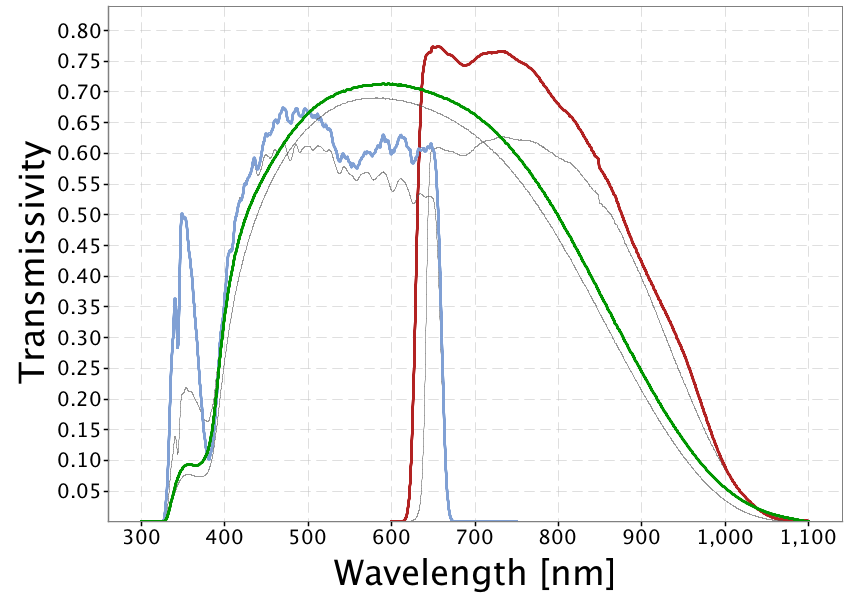
\includegraphics[scale=0.5]{GaiaDR2Passbands.png}
\caption{Filter response functions for Gaia photometric filters. Source: \protect\url{https://www.cosmos.esa.int/web/gaia/iow_20180316}}
\label{Gaia_response_funcs}
\end{center}
\end{figure}

\begin{figure}[h]
\begin{center}
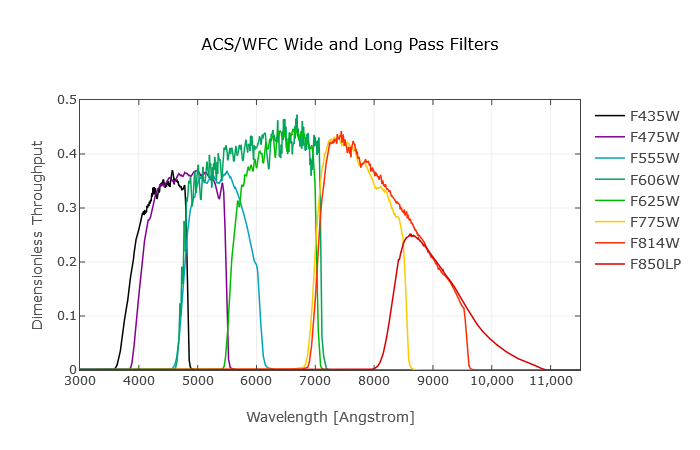
\includegraphics[scale=0.5]{ACS_Wide.png}
\caption{Filter response functions for wide-field ACS filters. Source: \protect\url{http://www.stsci.edu/hst/acs/analysis/throughputs}}
\label{ACS_response_funcs}
\end{center}
\end{figure}

\begin{figure}[h]
\begin{center}
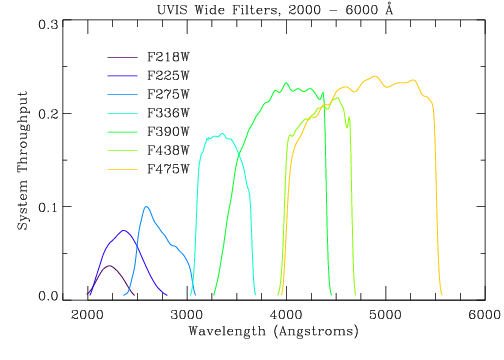
\includegraphics[scale=0.5]{UVIS_Wide1.jpg}
\caption{Filter response functions for wide-field WFC3 filters. Source: \protect\url{http://www.stsci.edu/hst/wfc3/ins_performance/throughputs/UVIS_filterthru.html}}
\label{WFC3_response_funcs1}

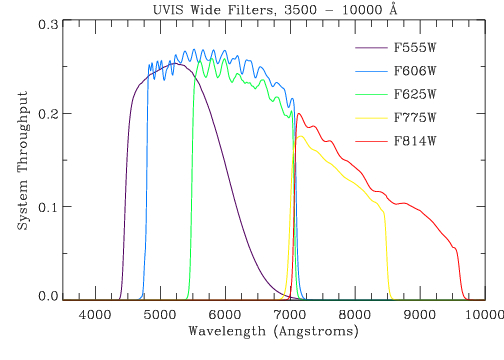
\includegraphics[scale=0.5]{UVIS_Wide2.jpg}
\caption{Filter response functions for wide-field WFC3 filters. Source: \protect\url{http://www.stsci.edu/hst/wfc3/ins_performance/throughputs/UVIS_filterthru.html}}
\label{WFC3_response_funcs2}
\end{center}
\end{figure}


The standard treatment of extinction is to apply a single constant value of the extinction coefficient for a given filter $X$, denoted in the literature by $A_{X}$. For wavelengths in or close to the optical spectral range, this quantity is usually expressed as a fixed ratio of the (constant) coefficient value in the Johnson-$V$ filter, the standard visual comparison filter.

\begin{table}
\begin{center}
\begin{tabular}{cccccc}
\hline
System & Filter & $\lambda_{\textnormal{cen}}$ / \AA & FWHM / \AA & $\lambda_{\textnormal{min}}$ / \AA & $\lambda_{\textnormal{max}}$ / \AA \\
\hline
% results: previously listed & from source website specified in caption					added more info: l_min & l_max
& F435W & 4359 & 881 & 3610 & 4860 \\ % & 4760 & 729
& F475W & 4781 & 1403 & 3863 & 5563 \\ % & 5000 & 986
& F555W & 5413 & 1236 & 4584 & 6209 \\ % & 5060 & 841
ACS & F606W & 5961 & 2255 & 4634 & 7180 \\ % & 6690 & 1566
& F625W & 6323 & 1390 & 5446 & 7100 \\ % & 6480 & 978
& F775W & 7763 & 1517 & 6804 & 8632 \\ % & 7320 & 1017
& F814W & 8117 & 2096 & 6885 & 9648 \\ % & 7460 & 1657
\hline
& F218W & 2216 & 329 & 1990 & 2603 \\ % & 2175 & 300
& F225W & 2341 & 464 & 1990 & 2968 \\ % & 2250 & 500
& F275W & 2696 & 417 & 2282 & 3119 \\ % & 2750 & 500
& F300X & 2722 & 660 & 2137 & 4098 \\ % &  & 2775
& F336W & 3368 & 550 & 3014 & 3707 \\ % & 3375 & 550
& F390W & 3929 & 951 & 3255 & 4470 \\ % & 3900 & 1000
WFC3 & F438W & 4322 & 674 & 3895 & 4710 \\ % & 4320 & 695
& F475W & 4768 & 1482 & 3942 & 5582 \\ % & 4750 & 1520
& F555W & 5262 & 1578 & 4381 & 7045 \\ % & 5410 & 1605
& F606W & 5941 & 2298 & 4700 & 7204 \\ % & 5956 & 2340
& F625W & 6274 & 1573 & 5414 & 7138 \\ % & 6250 & 1550
& F775W & 7725 & 1454 & 6869 & 8571 \\ % & 7760 & 1470
& F814W & 7814 & 1505 & 6978 & 9684 \\ % & 8353 & 2555
\hline
& G & 6631 & 4397 & 3321 & 10515 \\ % & 6730 & 4400
Gaia & G\textsubscript{bp} & 5330 & 2530 & 3283 & 6714 \\ % & 5320 & 2530
& G\textsubscript{rp} & 7896 & 2956 & 6296 & 10637 \\ % & 7970 & 2960
\hline

\end{tabular}
\caption{Basic properties of the filters employed in this project. See text for details. Source: \protect\url{http://svo2.cab.inta-csic.es/svo/theory/fps3/index.php}}
\label{filter_basics}
\end{center}
\end{table}

In Table \ref{filter_basics}, all the filters used for this project are listed. The name of each filter is displayed alongside its central wavelength ($\lambda_{\textnormal{cen}}$), full-width at half-maximum (FWHM) and the minimum ($\lambda_{\textnormal{min}}$) and maximum ($\lambda_{\textnormal{max}}$) detection wavelengths.****

Filters thus**** present a challenge when trying to determine stellar spectra accurately. This task is further complicated by the fact that, even in the wavelength range where a filter does detect incoming flux, the fraction of light it detects, known as the transmittance, is not uniform across the range. The transmittance as a function of wavelength is known as a transmission curve, bandpass or filter response function. Examples of response functions for some**** of the filters employed in this project are shown in Figure \ref{ACS_response_funcs}. By comparing these with the filters' information in Table \ref{filter_basics}, it can be seen that the exact shape of the response function could have a significant impact on the observed spectrum if not taken into account.
The values in the column labelled 'FWHM' represents the full width at half-maximum. In this case, it is defined as the difference between the lowest and highest wavelength values at which the transmittance value is half of its maximum value for the filter, typically assuming the response function can be approximated as a Gaussian distribution centred on the central wavelength. The FWHM acts as an approximate measure of the wavelength range within which the filter can reliably be used for observations.

The wavelengths of light visible to the average human eye are in the range 3800-7400 \AA . Hence, the filters used here cover wavelengths from the soft-ultraviolet (soft-UV) to the near-infrared (NIR),  including all visible wavelengths.



\chapter{Theoretical background}
While observations can reveal properties of individual stars and stellar populations more generally, the significance of these properties can only be gained by understanding the underlying physical processes and structure of the stars themselves. This chapter details the physical and mathematical framework of the processes which motivate and underpin this project.

\section{Stellar parameters} \label{params}
To understand the significance of differences between stars with respect to interstellar extinction, we must first define the fundamental features of a stellar atmosphere, which will be used in this project as the input variables on which any star-to-star variations in extinction will be modelled. \\*

\begin{figure}[h]
\begin{center}
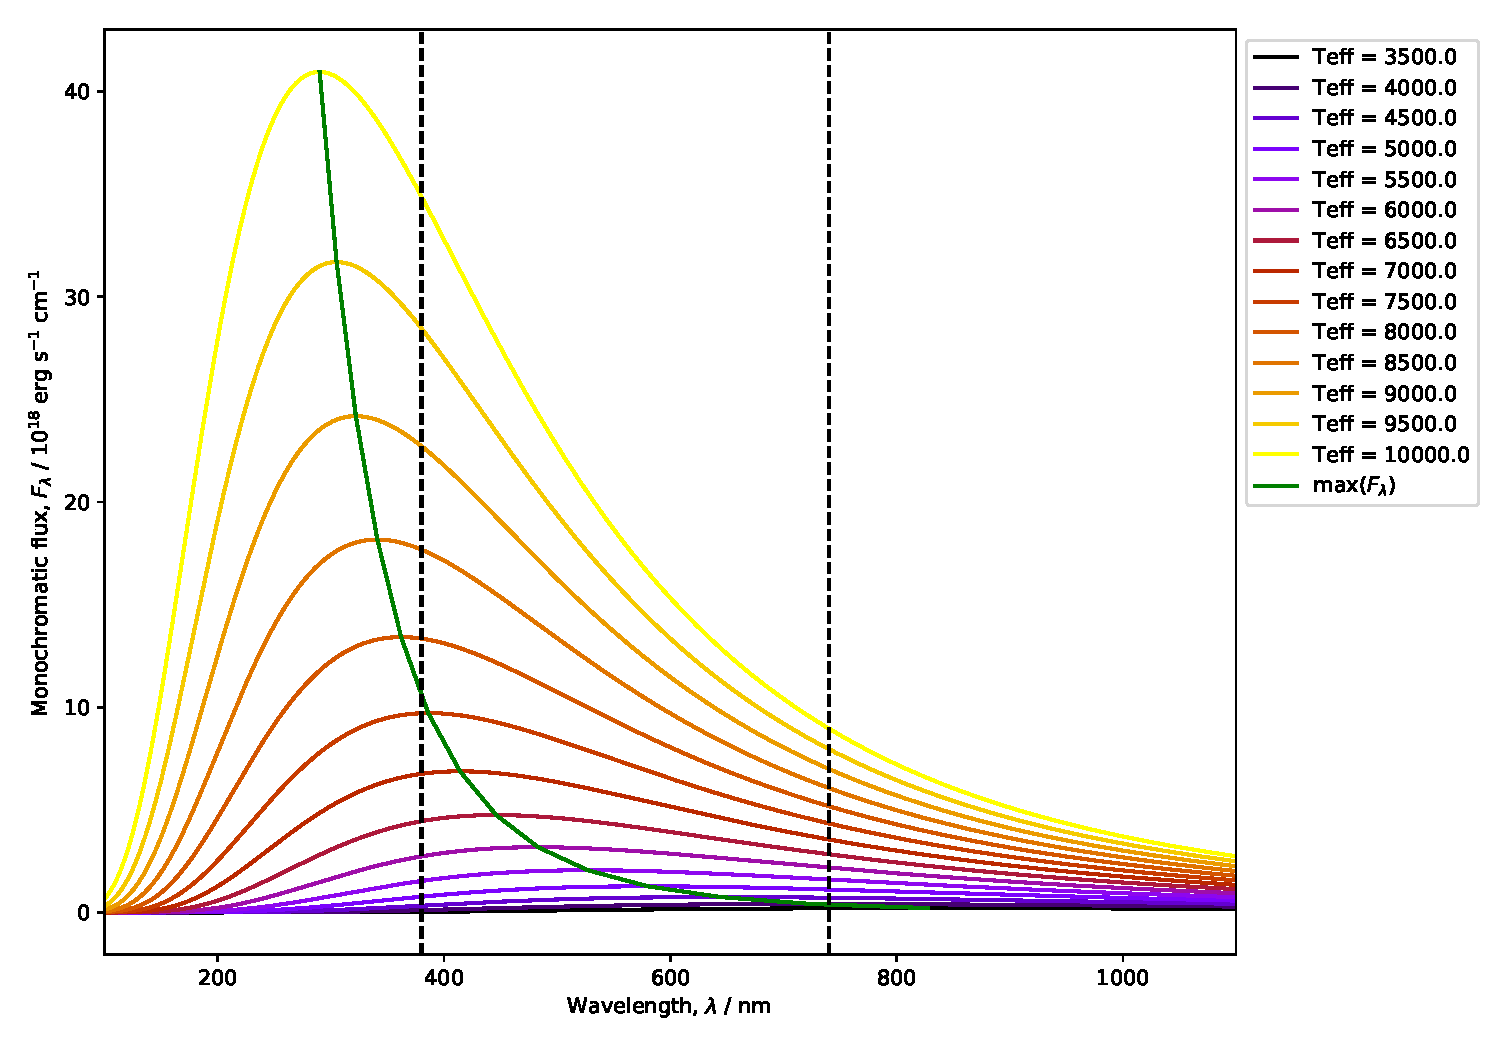
\includegraphics[scale=0.5]{blackbody_teff_illustration.pdf}
\caption{Monochromatic flux of a black body for different stellar effective temperatures. The black dashed lines mark the approximate limits of the visible part of the EM spectrum. The green curve represents the distributed of the maxima for the other curves.}
\label{planck_curve}
\end{center}
\end{figure}

The effective temperature ($T_{\textnormal{eff}}$) of a star is defined as the thermodynamic temperature of a black body which produces the same stellar flux across all wavelengths (known as the bolometric flux) as that produced by the star. A black body represents the perfect thermal emitting object. The universal equation of the radiation emitted by a black body produces the body's flux per unit wavelength per unit angular viewing area, $F_{\lambda,bb}$, known as the black body's monochromatic flux. The equation, known as the Planck Law, is as follows:


\begin{equation}
F_{\lambda,bb} = \frac{2hc^{2}}{\lambda^{5}\left(\exp\left({\frac{hc}{\lambda k_{B}T}}\right) - 1\right)}
\label{planck_bb}
\end{equation} 

where $T$ is the thermodynamic temperature of the black body, $h$ is Planck's constant, $c$ is the vacuum speed of light and $k_{B}$ is Boltzmann's constant. This equation also holds if the light wave frequency is used instead of the wavelength, with the monochromatic flux $F_{\nu,bb}$ now being the black body flux per unit frequency:

\begin{equation}
F_{\nu,bb} = \frac{2h\nu^{3}}{c^{2}\left(\exp\left({\frac{h\nu}{k_{B}T}}\right) - 1\right)}
\label{planck_bb_freq}
\end{equation}

In this project, the definition of monochromatic flux for any given object will be reserved exclusively for the flux per unit wavelength, $F_{\lambda}$, with any calculations involving black body fluxes using Equation \ref{planck_bb}. \\*

The general approximation of stars to black bodies (and hence the actual stellar surface temperature to $T_{\textnormal{eff}}$) is valid because all stars have been observed to have spectra that closely resemble those of black bodies, with the notable exception of atmospheric absorption lines.

\begin{equation}
L = 4 \pi R^{2} \sigma_{SB} T_{\textnormal{eff}}^{4}
\label{Teff_def}
\end{equation}

Effective temperature has an effect on interstellar extinction due to its strong effect on the stellar luminosity and, hence, the flux. For a higher flux, more photons are likely to interact with the ISM, hence a higher extinction coefficient. \\*

The metallicity of a star is defined as the fractional abundance of heavy elements, often approximated by iron (Fe) alone, relative to the star's hydrogen (H) abundance, compared to that of the Sun. The abundances are determined by the strength of the elements' characteristic atomic absorption lines in the stellar spectra.

\begin{equation}
\textnormal{[Fe/H]} = \log\left(\frac{N_{\textnormal{Fe}}}{N_{\textnormal{H}}}\right) - \log\left(\frac{N_{\textnormal{Fe},\odot}}{N_{\textnormal{H},\odot}}\right)
\label{FeH_def}
\end{equation}

For a generic atomic species $E$, $N_{E}$ represents its number density. For stellar observations, $N_{E}$ is measured at the surface. Since the output is logarithmic, a value of [Fe/H] = 0 indicates solar metallicity. An increase in metallicity would cause the corresponding absorption lines to be stronger, thus reducing the observable flux. An increased metallicity also implies an increase in abundance of sub-ferrous metals. The presence of more nuclear species, each with unique absorption line configurations, inevitably creates more observable lines, further increasing the apparent extinction in the spectral flux.\\*

The definition of the stellar surface gravity $g$ is simply the value of the standard Newtonian gravitational acceleration, applied to the stellar surface (the mass is the total stellar mass, $M_{*}$, and the distance is the stellar radius, $R_{*}$):

\begin{equation}
g = \frac{GM_{*}}{R_{*}^{2}}
\label{gravity_def}
\end{equation}

A greater surface gravity, as can be inferred from Equation \ref{gravity_def}, represents a surface with a higher mass density. For stars, being self-gravitating, this infers a higher atomic number density. The effects of surface gravity upon the emitted stellar spectrum arise directly from the effect of atomic number density on the quantum properties of the interactions between the photons and atomic electrons. \\*

Ideally, all photons would have a single exact wavelength and energy, and all electrons in a given atomic occupancy level would only be able to absorb and emit such photons. However, Heisenberg's uncertainty principle implies both a fundamental uncertainty in a particle's velocity and a direct impact of this uncertainty on the uncertainty of the particle's momentum. It can be easily shown, particularly in the case of photons, that the pairing of the particle's energy (uncertainty $\Delta E$) and time ($\Delta t$) share these same uncertainty properties. This results in the following relation:

\begin{equation}
\Delta E \Delta t \geq \hbar/2
\label{heisenberg}
\end{equation}

When a particle absorption a photon, the absorption process is not instantaneous and therefore carries an uncertainty in the time taken for the process to be completed, with a corresponding uncertainty in energy. Across a large number of absorptions for the same initial electron state, the result is a spread in the energies of the absorbed photons. The associated emission line is therefore broadened by the multiple wavelengths of the photons. This is universal and referred to as ``natural broadening''.\\*

The impact of surface gravity arises via additional broadening effects upon these same absorption lines. When broadening effects are applied to an emission spectrum, such as a spectrum from a stellar surface, the result is that fewer photons pass through the surface, thereby reducing the surface flux seen by an outside observer. \\*

%A local environment in which atoms or ions are more closely spaced leads to more frequent interactions between the particles. Shorter timescales mean an increase in the fraction of atoms which collide while one of their electrons is absorbing a photon. Since collisions change the states of both atoms, the electron occupancy levels also change. Therefore, these electrons will only interact with photons at different energies, and therefore wavelengths, during the collision. This means that a large sample of atoms, all of the same atomic species and containing the same configuration of electrons, is more able to absorb photons in a wider wavelength range. \\*

Additional broadening effects are caused by processes whose impact is dependent on the separation between interacting atoms and ions and hence on the atomic/ionic number density. The broadening is due to the perturbations induced by these processes on the Hamiltonian quantum operator for the system \citep{1929ApJ....69..173S}, which produces shifts in the associated energy eigenvalues. The broadening impact of each process obeys a distance law for a particular integer value of the index $p$ \citep{Peach_1984}:

\begin{equation}
\Delta \lambda \propto r^{-p}
\label{broadening_dist}
\end{equation}

where $p$ is a positive integer. A local environment of higher number density, in which atoms are more closely spaced, increases the frequency of interactions between atoms/ions and the likelihood of multiple processes contributing significantly to the total broadening effect. \\*

The scenarios $p = 2$ and $p = 4$ are due to the linear and quadratic Stark effects, respectively. The Stark effect represents a perturbation in the quantum-mechanical potential of the electron due to the influence of an external electric field, $F$. The linear (first-order) Stark perturbation is proportional to $F$ and dominates the broadening for weak fields, while the quadratic (second-order) effect is proportional to $F^{2}$ and dominates for stronger fields. For free electrons and ions with charge number $Z$, which can be treated as point sources of charge, $F \propto Z/r^{2}$, giving the stated $p$ values for the linear and quadratic. This relation also gives the field strength dependence on number density, $N$: $F \propto N^{2/3}$.\\*

For interactions between neutral atoms, the relevant processes are the standard van der Waals interaction ($p = 6$) and the so-called ``resonance broadening'' effect ($p = 3$), which is only valid for two atoms of the same type, with one of these atoms required to be in the ground state \citep{1969A&A.....3..462L}. Resonance broadening is weaker at higher densities due to the influence of multiple neighbouring atoms cancelling the individual perturbations \citep{10.2307/96756}. \\*

%This effect, known as ``collisional broadening'', causes a Lorentzian distribution of absorption energies (and wavelengths) about the normal emission energy for that particular electron state. \\*

% END OF ???

Also, the rotation of the star has an impact on spectral line widths via a Doppler shift at each line-of-sight velocity. Together, the distribution of these velocities has the effect of broadening the absorption lines via a Gaussian distribution in wavelength, centred on the  \citep{1995ApJ...439..860C}. The relationship to surface gravity arises from the gravity being the source of centripetal acceleration at the surface of a rotating star, and therefore being proportional in magnitude to the square of the surface rotational velocity.

\section{Extinction definition} \label{extinc_desc}
Extinction is defined using the standard astronomical system of flux magnitudes. In general, the difference between two flux measurements, $f_{1}$ and $f_{2}$, in magnitudes, is expressed as:

\begin{equation}
\label{mags_def}
m_{1} - m_{2} = -2.5\log \left( \frac{f_{1}}{f_{2}} \right)
\end{equation}

where $m_{1}$ and $m_{2}$ are the magnitudes for $f_{1}$ and $f_{2}$, respectively. However, the flux of a source varies intrinsically with the distance travelled by the light to the observer (see Equation \ref{flux_def}). To account for this, the distances to sufficiently close sources can be determined independently of their flux by measuring the sources' parallax from Earth. \\*

The parallax $p$ of an object is defined as the angular distance the object moves relative to the ``fixed'' background stars as the Earth moves a distance of 1AU (the average separation of the Sun and Earth during one complete orbit) perpendicular to the line-of-sight. This allows the distance, $d$, to be calculated using the geometry of triangles, combined with the small-angle approximation, as:

\begin{equation}
d/\textnormal{pc} = \frac{1}{(p/\textnormal{arcsec})}
\end{equation}

For more distant stellar sources with much smaller parallaxes, a potential alternative is to view the object in a very long-wavelength filter, in which observations are likely to be impacted much less significantly by extinction, to estimate the type of star being observed, before using theoretical models to compare with observations at different wavelengths. This is more effective for brighter stars. \\*

The role of distance gives each astronomical object two principal flux parameters. These are the apparent magnitude, $m$, and the absolute magnitude, $M$. The apparent magnitude is the flux magnitude of a source as observed by the telescope. The absolute magnitude is the predicted flux magnitude of the same source if it were to be placed at a fixed distance of 10 parsecs (pc) from the telescope with zero extinction. The absolute magnitude exists for the purpose of stellar classification, as the corresponding flux is simply a constant multiplied by the stellar luminosity (see Equation \ref{flux_def}), which is an intrinsic physical property of the star. \\*

However, to calculate the absolute magnitude of a source, we first require its distance and extinction coefficient, $A$. To account for extinction, it is necessary to define a new quantity, known as the intrinsic apparent magnitude, $m_{0}$. This is defined as the flux magnitude of a source corrected for losses due to extinction but not due to distance. In practice, it represents the apparent magnitude for light passing through a fully-transparent medium. The relation between $m_{0}$ and $M$, can be found by combining Equations \ref{flux_def} and \ref{mags_def}:

\begin{equation}
\label{distance_modulus}
m_{0} - M = -2.5\log \left( \left(\frac{10\textnormal{pc}}{d}\right)^{2} \right) = 5\log\left(\frac{d}{\textnormal{pc}}\right) - 5
\end{equation}

This quantity is known as the distance modulus. As seen in Equation \ref{distance_modulus}, it varies only with distance. The quantity $m - M $, linking the initial observed data with the final theoretical data, is known as the apparent distance modulus and varies with both distance and extinction. \\*

Therefore, the extinction coefficient $A$, defined as the flux lost due to the effects of the intervening line-of-sight medium, can be defined as:

\begin{equation}
\label{bol_extinc}
A = m - m_{0}
\end{equation}

This fits with the physical definition of interstellar extinction given earlier, i.e. as the flux lost solely due to scattering and absorption in the interstellar medium. \\*

The object of this project is to compare different extinction treatments and the subsequent effect on the interpretation of observational cluster datasets. For any observational set of stars, the stars' extinction coefficients will be completely unknown from the data alone. In order to compare observational and theoretical  data, the most convenient approach is to add the (theoretical) extinction coefficient(s) to the theoretical dataset magnitudes (i.e., absolute magnitudes), before comparing to the distance-corrected observational data. As a result, the quantity from each dataset that is being compared is the absolute magnitude plus the extinction coefficient. If we label this quantity $M_{\textnormal{ext},X}$ for a given filter, we can define it as:

\begin{align}
\begin{split}
M_{\textnormal{ext},X} &= M_{X} + A_{X} \textnormal{ (theoretical data)}\\
 &= m - (m - M)_{X,0} \textnormal{ (observational data)}
\end{split}
\label{MextX_eq}
\end{align}


However, as noted earlier, in astronomy it is not feasible to attempt observations by a single instrument at all wavelengths. Telescopes instead are purpose-built to study a single wavelength range within the full EM spectrum. Within this range, telescope observation ranges are further divided by filters or passbands, one of which is placed on their aperture at any given observation time. As shown in Figures \ref{ACS_response_funcs}-\ref{Gaia_response_funcs}, any single filter $X$ has a limited range of wavelengths for which it is able to detect flux. It can also be seen in these figures that the transmittance of the filter changes as a function of wavelength. These instrumental factors must be considered, in addition to the observational challenges of distance and interstellar extinction, in order to correctly analyse observation telescope data. \\*

%\begin{figure}[h]
%\begin{center}
%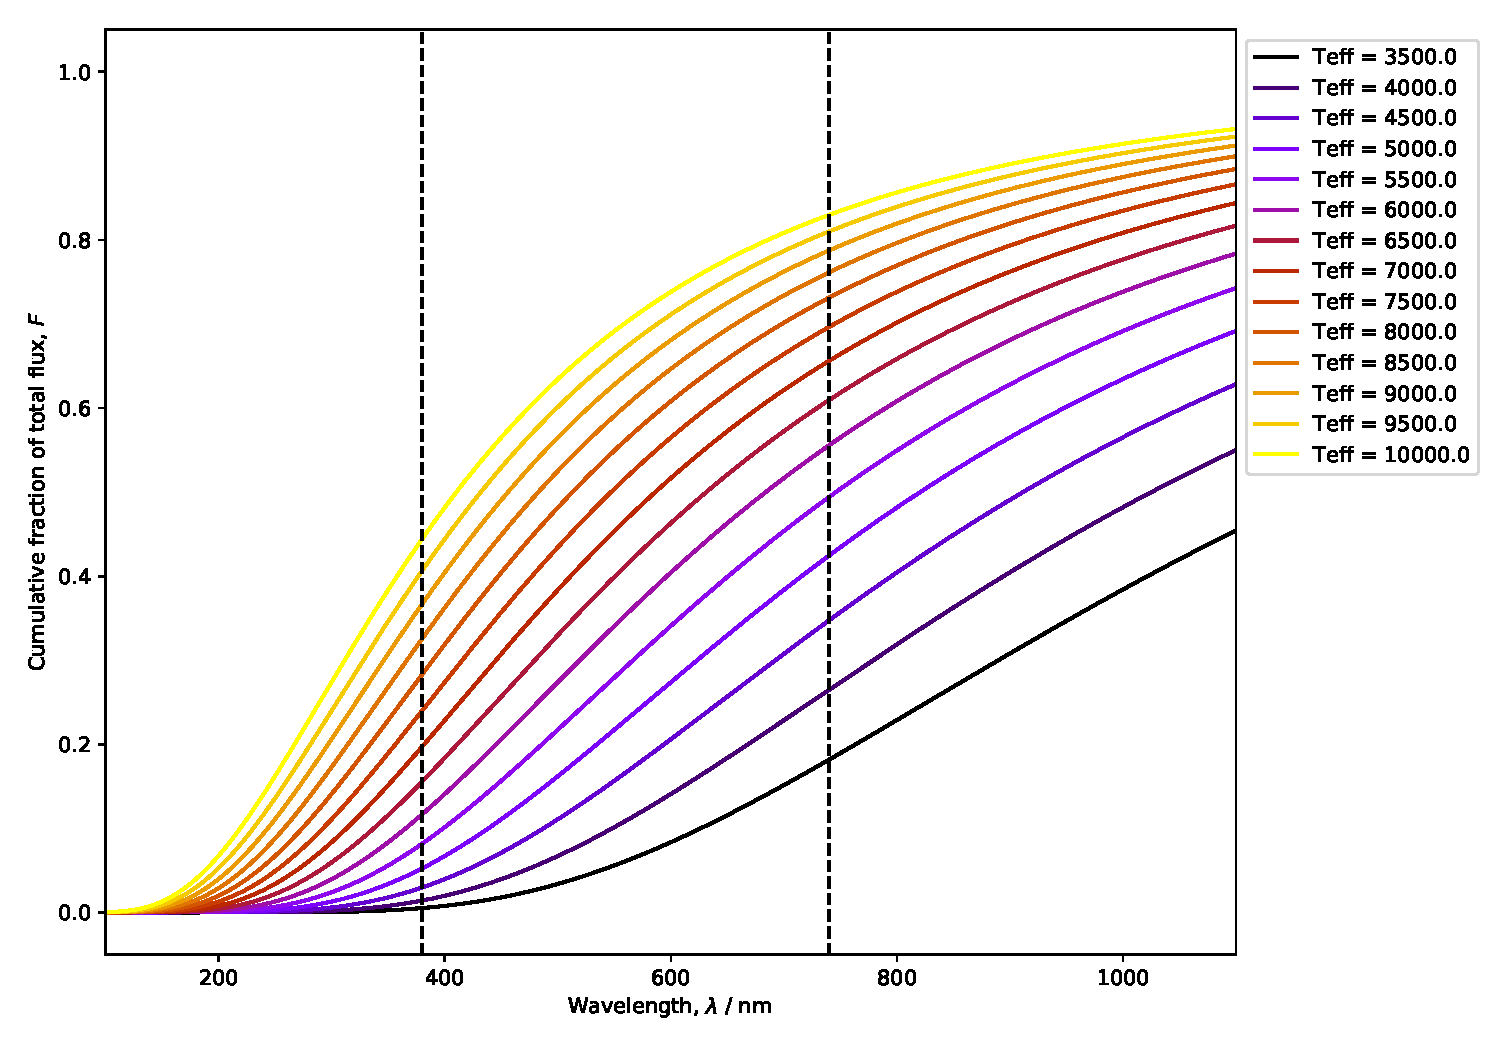
\includegraphics[scale=0.5]{cumulative_blackbody_teff_illustration.pdf}
%\caption{****Cumulative fraction of the total flux of a black body for different stellar effective temperatures. The black dashed lines mark the approximate limits of the visible part of the EM spectrum.}
%\label{cumulative_planck_curve}
%\end{center}
%\end{figure}

If we compare the individual black body spectra in Figure \ref{planck_curve}, it can be seen that the maximum monochromatic flux of the black body occurs at an increasingly shorter wavelength for objects with increasingly higher temperatures. This makes the object appear bluer to an observer. The relationship between the wavelength at which the monochromatic flux is maximal ($\lambda_{max}$) and the black body temperature is quantified by Wien's displacement law:

\begin{equation}
\lambda_{max} T = 2.898 \times 10^{6} \textnormal{ nm K}
\label{wien_eq}
\end{equation}

More importantly, for two wavelength regions which are sufficiently far apart, the change in flux between the regions is always greater for stars with higher effective temperatures. Therefore, to measure a star's effective temperature, observers compare the star's observed flux in two filters operating at different wavelengths within the UV-IR wavelength range. The difference between the star's flux magnitudes in each of the two filters is then taken, with the flux in the redder filter being deducted from that of the bluer filter. This quantity is known as the colour index. For two filters $X$ and $Y$, with $X$ being bluer than $Y$, the colour index of observations made using those filters, $(X-Y)$, is defined as:

\begin{align}
\begin{split}
(X-Y) &= m_{X} - m_{Y} \\
 &= (m_{X,0} - m_{Y,0}) + (A_{X} - A_{Y}) \\
 &= (X-Y)_{0} + E(X-Y)
\end{split}
\end{align}

where $(X-Y)_{0}$ is the true or intrinsic colour index of the object and $E(X-Y) = A_{X} - A_{Y}$ is known as the colour excess, but can also be denoted in literature using the term ``reddening''. A major advantage of using the intrinsic colour index over absolute magnitudes is that it is completely independent of distance. The colour excess represents the effect of extinction on the observed colour index. Its importance arises from the prominence of the intrinsic colour index in determining effective temperature. Higher values of $(X-Y)$ indicate redder stars, with lower effective temperatures. \\*

The most commonly-used colour index, employed as a reference for most optical observations, is the Johnson ($B-V$) index. This is due to these filters being the among most long-lived, well-used and best-studied available, allowing for better comparisons of different data, including data from older archives. \\*

Due to the potential confusion due to the use of the term ``reddening'' for both $A_{X}$ and $E(X-Y)$ in literature, $A_{X}$ will be referred to here as the ``extinction'' or ``extinction coefficient'' and $E(X-Y)$ as the ``colour excess''.

\section{Bolometric corrections} \label{BC_theory}
All the equations in Section \ref{extinc_desc}, including those for extinction, are not useful when applied to telescopes, as any filter will only detect a small fraction of the bolometric stellar flux that reaches the telescope. The missing information resulting from this observational constraint renders it difficult to determine the interstellar extinction. These constraints much be mitigated before an accurate value of the extinction coefficient can be determined. This mitigation is carried out by employing bolometric corrections.\\*

The use of bolometric corrections requires the detailed knowledge of stellar spectra least susceptible to significant extinction, i.e., nearby stars with high apparent fluxes. Only with complete knowledge of the spectrum from a reference star can the true spectrum of a distant star with unknown extinction be calculated. The spectra of these stars can be computed by using a grid of predicted fluxes from a stellar atmosphere model, the grid being composed of the stellar parameters known to change emission in stellar atmospheres. These are effective temperature, surface gravity and metallicity. For all filter systems studied in this project, the nearby bright star Vega ($\alpha$ Lyr) was used as the reference object. Using Vega as the reference star is the most well-known approach to photometric calibration \citep{2014MNRAS.444..392C}.\\*

After accounting for a general extinction effect on an object's emission, its apparent magnitude in the wavelength range of a given filter $X$, defined as increasing from the shortest ($\lambda_{1}$) to the longest ($\lambda_{2}$) wavelength for which its response function is non-zero, can be calculated as:

\begin{equation}
m_{X} = -2.5 \log_{10} \left(\frac{ \int_{\lambda_{1}}^{\lambda_{2}} f_{\lambda} \left( 10^{-0.4 A_{X,\lambda}} \right) S_{\lambda} d\lambda }{ \int_{\lambda_{1}}^{\lambda_{2}} f_{\lambda}^{0} S_{\lambda} d\lambda }\right) + m_{X}^{0}
\label{app_mag_def}
\end{equation}

where $f_{\lambda}$ represents the (theoretical) monochromatic flux at a given wavelength $\lambda$ at the observer distance from the source, $A_{X,\lambda}$ is the extinction coefficient in $X$ as a function of wavelength and $S_{\lambda}$ represents the filter response function of $X$. $f_{\lambda}^{0}$ and $m_{X}^{0}$ represent the monochromatic flux and apparent magnitude, respectively, in $X$of a known reference object, which is Vega in the case of this project.

%Since our goal, ultimately, is to document potential effects of fundamental stellar properties upon observables, we need to connect the observational and idealised scenarios, for which we use bolometric corrections.

To derive the equation linking a bolometric correction with the extinction parameter, we start with the definition of a bolometric correction in a filter $X$, which is denoted by $BC_{X}$:

\begin{equation}
BC_{X} \equiv M_{\textnormal{bol}} - M_{X}
\label{BC_def}
\end{equation}

where $M_{X}$ is the absolute magnitude of the object in $X$ and $M_{\textnormal{bol}}$ is its (predicted) absolute bolometric magnitude, defined relative to the Sun using:

\begin{equation}
M_{\textnormal{bol}} = M_{\textnormal{bol},\odot} - 2.5 \log_{10} \left( \frac{4\pi R^{2}F_{\textnormal{bol}}}{L_{\odot}} \right)
\label{mbol_sun}
\end{equation}

where  $F_{\textnormal{bol}}$ is the bolometric stellar flux at its surface, $R$ is the stellar radius, $M_{\textnormal{bol},\odot}$ is the solar absolute bolometric magnitude, which is assumed in this work to have a value of 4.75 and $L_{\odot}$ is the solar luminosity, for which a value of $3.844 \times 10^{33}$ erg s$^{-1}$ is used. Bolometric corrections can be expressed as a function of extinction using the universal definition of $M_{X}$ in terms of $m_{X}$ and the distance $d$ to the source:

\begin{equation}
M_{X} = m_{X} - 2.5 \log_{10}\left( \left( \frac{d}{10 \textnormal{pc}} \right)^{2} \right),
\label{abs_mag_def}
\end{equation}

together with the equation $f_{\lambda}d^{2}=F_{\lambda}R^{2}$, where $F_{\lambda}$ is the monochromatic flux at $\lambda$ at the stellar surface. This gives the final function for a bolometric correction for filter $X$:

\begin{align}
\begin{split}
BC_{X} &= M_{\textnormal{bol},\odot} - m_{X}^{0} - 2.5 \log_{10} \left( \frac{4\pi R^{2}F_{\textnormal{bol}}}{L_{\odot}} \right) \\
&+ 2.5 \log_{10} \left( \frac{\int_{\lambda_{1}}^{\lambda_{2}} F_{\lambda} \left( 10^{-0.4 A_{X,\lambda}} \right) S_{\lambda} d\lambda}{\int_{\lambda_{1}}^{\lambda_{2}} f_{\lambda}^{0} S_{\lambda} d\lambda} \right)
\label{BC_extinc}
\end{split}
\end{align}

For a filter $X$, the extinction parameter $A_{X} = A_{X,\lambda}$ must be calibrated relative to a known value. In this work we will input a value of the extinction in the well-studied Johnson-$V$ filter, $A_{V}$. To extract $A_{X}$, we use the simple relation:

\begin{equation}
A_{X,\lambda} = \left( \frac{A_{X,\lambda}}{A_{V}} \right) A_{V}
\label{ratio_eq}
\end{equation}

together with the chosen value of $A_{V}$ (for this project the values were $A_{V} = 0$, 1 - note that $BC_{X}(A_{V}=0)$ essentially assumes no extinction in any filter), before taking the difference between the two $BC_{X}(A_{V})$ outputs, giving the following equation:

\begin{align}
\begin{split}
BC_{X}(0) - BC_{X}(A_{V}) &= 2.5 \log_{10} \left( \frac{\int_{\lambda_{1}}^{\lambda_{2}} F_{\lambda}  S_{\lambda} d\lambda}{\int_{\lambda_{1}}^{\lambda_{2}} F_{\lambda}\left( 10^{-0.4 \left(A_{X,\lambda}/A_{V}\right) A_{V}} \right) S_{\lambda} d\lambda} \right) \\
&\approx \left(A_{X}/A_{V}\right)
\label{BCs_diff}
\end{split}
\end{align}
%\\ &\approx \left(A_{X}/A_{V}\right)A_{V}

As demonstrated in the equation above, any dependence of the $A_{X}/A_{V}$ data on the Vega measurements or (as yet unknown or uncertain) bolometric quantities from Equation \ref{BC_extinc} is eliminated during the subtraction. \\*

Most papers employing filters in the relevant spectral regions use the model of $A_{\lambda}/A_{V}$ as described by \cite{1989ApJ...345..245C} or a modified version (\cite{1994ApJ...422..158O} and \cite{1999PASP..111...63F} are among the most frequently used). This project uses the original model. The assumptions used to equate $A_{X}/A_{V}$ with the result of Equation \ref{BCs_diff} are valid because the observational flux data used by \cite{1989ApJ...345..245C} when deriving their monochromatic extinction model were obtained using broad-band filters, and so are subject to the effects of variations inherent in both the real stellar spectra and the filter response functions, making the data heterochromatic \citep{2014MNRAS.444..392C}, in the same manner as the output data. \\*

\section{Forbes effect}
The Forbes effect occurs as a broadband beam of light, such as that passes through an extended partially-transparent medium, such as a series of glass plates, the Earth's atmosphere or an interstellar gas cloud. It states that the greater the distance travelled by a light beam through the medium, the more penetrating the beam becomes \citep{1842RSPT..132..225F}. If we use the case of the glass plates as an example, this means that the fraction of the light incident on the $n$th plate in the series which is dissipated by that plate from the original path is always greater than the corresponding fraction at the ($n+1$)th plate \citep{1995A&AS..109..293G}. The physical basis for the Forbes effect is that those photons in the original beam with wavelengths that make them the most likely to be absorbed or refracted are separated from the beam earlier. Therefore, as the beam travels through the medium, its constituent photons are progressively less likely to be separated. Since a higher fraction of its photons are retained as the distance through the medium increases, the beam is more penetrating \citep{OHVRIL1999305}.\\*

The Forbes effect thus has an impact on the non-zero $A_{V}$ value used in Equation \ref{BCs_diff} because if a uniform medium is assumed, as here, where $R_{V}$ is held constant at the standard diffuse ISM value of 3.1 \citep{1989ApJ...345..245C}, a larger $A_{V}$ value implies a longer path through the ISM, and thus a stronger Forbes effect. According to \cite{2008PASP..120..583G}, any significant impact from the Forbes effect on the values of $A_{X}/A_{V}$ occurs for a chosen $A_{V} \gtrsim 4$. They found that the effect was particularly strong for stars with $T_{\textnormal{eff}} \lesssim 3000$K and that, unsurprising, it became greater as the wavelength range covered by the filter response function increased. The choice of $A_{V} = 1$ made for this project should avoid serious problems from the Forbes effect, even for the widest filters.


\section{Basics of stellar evolution} \label{stel_evol}
It can be seen from Equation \ref{Teff_def} that the luminosity (and therefore flux) of a star is dependent on radius as well as effective temperature. If a plot is made of luminosity against effective temperature (known as a Hertzsprung-Russell diagram), it can be seen that all stars in a given population follow a single track. Because the stars are approximately the same age, this track is know as an isochrone. Isochrones for different population ages and metallicities are calculated using theoretical stellar models for the largest possible spread of initial stellar masses. An isochrone in the HR diagram has a number of distinct features:

\begin{itemize}
\item Most stars, including the coolest and least-luminous objects, follow a tight pattern of luminosity increasing with temperature. This is known as the main sequence (MS).
\item This pattern stops as the luminosity continues to increase slowly but with decreasing temperature. The upper end of the MS is called the main-sequence turn-off (MSTO), which is followed by the sub-giant branch (SGB).
\item After the SGB, the gradient becomes much steeper, with temperate decreasing slowly and luminosity increasing rapidly. This is the red-giant branch (RGB).
\item At the tip of the RGB, stars start becoming fainter and their temperatures increase. Eventually, their is a sequence of stars with near-constant luminosity but a range of effective temperatures. This is the horizontal branch (HB).
\item After the horizontal branch, there is again a rapid increase in luminosity accompanied by a slow decrease in temperature. This is the asymptotic giant branch (AGB).
\end{itemize}

Stars with higher initial mass have shorter lifetimes for each evolutionary stage, due to their correspondingly higher temperatures, which increases the nuclear fusion efficiency. This causes higher surface luminosities. On the main sequence, therefore, more massive stars appear in the upper-left part and leave the MS earlier, which is the physical cause of the MSTO. As a population ages, the MSTO moves down the MS as progressively less-massive stars leave the MS. \\*

On the main sequence, nuclear fusion occurs in the core and any products must be subjected to mixing effects to reach the atmosphere. Since stellar interiors are physically fluid, heavier nuclei, which are more dense, preferentially gather in regions close to the star's centre of gravity. Therefore, processes such as convection, thermohaline mixing and radiative levitation are required to induce a noticeable change in surface composition. However, these processes require certain physical conditions on local scales, if they are to be sustained for long enough to induce a visible change in the stellar spectrum. \\*

On the main-sequence, only low-mass stars ($M_{*} \lesssim 0.38M_{\odot}$) \citep{2018A&A...619A.177B} have fully-convective interiors. Massive ($M_{*} \gtrsim 1.5M_{\odot}$) stars have convective cores, but radiative envelopes. Intermediate-mass stars, including the Sun, have radiative cores and convective envelopes. Since regions in which energy transport is dominated by radiative effects are stable against convection \citep{2017RSOS....470192S}, stars with masses greater than $0.38M_{\odot}$ are highly unlikely to show large changes in atmospheric composition along the main sequence. However, the fully-convective lower-mass stars are able to do so. Therefore, the faintest and reddest parts of the main sequence are most likely to have atmospheres enriched with metals, which would be confined in the cores of more massive stars. These enriched atmospheres are therefore highly sensitive to the overall metallicity of the original gas cloud in which the star, and its parent cluster if applicable, formed.

\begin{equation}
\nabla_{\textnormal{rad}} = \frac{3\kappa LP}{16\pi acGmT^{4}}
\end{equation}

To illustrate, let us consider a bubble of gaseous material in pressure-equilibrium with its surroundings and represent mixing as a significant change in the bubble's (radial) position on a significant time-scale, arising from small differences in the remaining 3 thermodynamic quantities between the bubble and its surroundings. For a non-rotating star, using a simple linear approach, together with the Archimedes principle, gives a set of 4 homogeneous differential equations for the (small) differences in $P$, $T$, $\mu$ and $r$ (Equations (3.1)-(3.4) in \cite{2017RSOS....470192S}). If $\Delta x_{i}$ are the differences in the 4 parameters, taking the ansatz form $\Delta x_{i} = B_{i} e^{nt}$ allows for a solution as a 3rd-order polynomial in $n$ (Equation (3.5) in \cite{2017RSOS....470192S}), if the determinant of the relevant matrix (dependent of the values of the $B_{i}$) is zero. The Routh-Hurwitz stability criterion can then be applied to this polynomial to give a general solution for $n$. For a physically-unstable solution, the exponent in the $\Delta x_{i}$ equation must be positive, i.e. $n$ must satisfy the condition $\operatorname{Re}(n) > 0$. Hence, the subsequent constraints on the polynomial coefficients form all the possible conditions for instability,  of which at least one must be satisfied. These constraints take the following form:

\begin{align}
\nabla _{\mu} &< 0 \label{mu_inv_ineq} \\
\nabla _{\textnormal{rad}} &> \nabla _{\textnormal{ad}} \label{schwarz_ineq} \\
\nabla _{\textnormal{rad}} &> \nabla _{\textnormal{ad}} + \left( \frac{\phi}{\delta} \right) \nabla _{\mu} \label{ledoux_ineq}
\end{align}

where $\nabla _{\mu} = d\ln\mu / d\ln P$, $\nabla _{\textnormal{rad}} = \left(\partial\ln T / \partial\ln P \right)_{\textnormal{rad}}$ and $\nabla _{\textnormal{ad}} = \left(\partial\ln T / \partial\ln P \right)_{\textnormal{ad}}$ are the temperature-pressure gradients for the local environment (dominated by radiation pressure) and the bubble (treated as an adiabatic ideal gas), respectively, $\phi = \left( \partial \ln\rho / \partial \ln\mu \right)_{P,T}$ and $\delta = -\left( \partial \ln\rho / \partial \ln T \right)_{P,\mu}$  \citep{1980A&A....91..175K}. \\*

In stellar evolution, the stages described above represent extended periods of time in which the stellar interior, described in theoretical models as a series of (quasi-)spherical shells, can be described as being in hydrostatic equilibrium, i.e., the gravitational pressure inwards on material in a given shell, due to the mass enclosed by the shell, is equal to the radiation pressure outwards generated by nuclear fusion occurring within the area enclosed by the shell, either in the core or in an inner shell. Giant stars are objects with luminosities significantly higher and surface gravities lower than stars on the main sequence (which generally have gravities in the range 4 $\lesssim$ log($g$) $\lesssim$ 5.5). \\*

\section{Colour-magnitude diagrams}

By examining the flux-magnitude equations from Section \ref{extinc_desc}, it becomes clear that both the absolute filter magnitudes and the intrinsic color indices can be used, together with bolometric corrections, to calculate the axis parameters of the HR diagram from observational data. To determine the detailed properties of stellar populations, all stars in an observational sample or star cluster are plotted together on a pair of axes known as a colour-magnitude diagram (CMD), which represents an observational analogue of the HR diagram. The absolute magnitude of stars in a given filter $Z$, $M_{Z}$, is on the y-axis, with the flux increasing (and the magnitude value decreasing) upwards. The intrinsic colour index of the stars in two filters $X$ and $Y$, $(X-Y)_{0}$, is on the x-axis, with the values increasing (and stars becoming redder) to the right. In practice, due to the unknown extinction coefficients of the individual stars and the cluster as a whole, the axial parameters  are $M_{\textnormal{ext},Z}$ and $(X-Y)$. Note that filter $Z$ may be the same as either $X$ or $Y$. \\*

In practice, the universal general shape and position of stellar populations in the HR diagram and each observational CMD, particularly the position and shape of the main sequence, provides a highly useful tool for comparing stellar populations with unknown distances and extinction coefficients to known examples and to theoretical models. This is done by alignment of the respective main sequences in CMDs, particularly the upper main sequence, which contains the most luminous MS stars and is less sensitive to the (initially unknown) value of the cluster metallicity than the lower MS. \\*



\chapter{Previous studies into extinction variations}

Although interstellar extinction at optical wavelengths has always
\cite{1989ApJ...345..245C} used observations of mostly ****bright O- and B-type main-sequence stars to produce empirical equations describing the mean ratio of extinction coefficients at a specific wavelength $\lambda$ ($A_{\lambda}$) to the extinction in the Johnson-$V$ filter ($A_{V}$), respectively. From this point onward, this ratio will be referred to as $A_{\lambda}/A_{V}$. They produced a basic universal equation of the form:

% avoided the complications of using reddening (which is not itself intrinsic and whose implications be impacted by the choice of filters) by 

\begin{equation}
A_{\lambda}/A_{V} = a(x) + b(x)/R_{V},
\label{CCM_general}
\end{equation}

where $x \equiv 1/\lambda$ and $R_{V} \equiv A(V)/E(B-V)$. The significance of $R_{V}$, as noted in the same paper, comes from its usefulness as an indicator of the nature of the interstellar medium through which the observed light travels in order to reach the observer.**** The total wavelength range was divided into 4 sub-ranges, each with a governing pair of empirically-determined equations (to determine $a(x)$ and $b(x)$, respectively). This model underpins more recent studies of intrinsic effects on extinction (\cite{2008PASP..120..583G}, \cite{2018MNRAS.479L.102C}), and provides the basis for the synthetic $A_{X}/A_{V}$ datasets in this project, where $A_{X}$ is the coefficient for a given filter $X$. Equation \ref{CCM_general} has become a standard model for observers to employ when observing in the UV, optical and near-IR wavelength regions, although it is not always accurate. \cite{1999PASP..111...63F} found that, due to the broadband nature of the Johnson filters and the general decrease of extinction with wavelength, the CCM relations overestimate the extinction in the near-IR and blue-visible Johnson filters. However, in the UV region covered by  the \cite{1989ApJ...345..245C} equations, the equations are accurate for 93\% of a homogeneous UV observational database \citep{2004ApJ...616..912V}.**** \\*

\cite{2008PASP..120..583G} produced data tables of $A_{X}/A_{V}$ via bolometric corrections (as was carried out in this study). for stellar atmosphere models with parameters $T_{\textnormal{eff}}$, log($g$) and [Fe/H]. They carried this out using the same ATLAS9 data \cite{2004astro.ph..5087C} that was used to generate the data for this project, but also combining it with data from other studies**** \cite{2002A&A...391..195G}, resulting in data covering a parameter space extending beyond the ATLAS9 limits in all three parameters. They used the data tables to directly**** calculate the $A_{X}/A_{V}$ values for the stellar models in theoretical isochrones****. While determining that the values of $A_{X}/A_{V}$ varied significantly with $T_{\textnormal{eff}}$ and log($g$), the variation with metallicity was found to be ~0.17$\%$ between [Fe/H] = 0.0 and [Fe/H] = -2.5. They found that, when they set $A_{V} = 6$, there was a systematic shift for the ACS system between extinction values calculated star-wise using the BC tables and a constant extinction value. The constant values of $A_{X}/A_{V}$ were calculated from a yellow dwarf in the low-extinction regime. Overall, the BC tables produced a smaller extinction coefficient in the F814W filter and a larger (F475W-F814W) colour index value. It also caused a change in the shape of the curve at the MSTO. They then applied the BC table data method to the case of the globular cluster M92. They found the optimal metallicity to be $Z = 0.0004$ ([Fe/H] $\approx$ -1.6) instead of the value obtain by previous observers of $Z = 0.0001$ ([Fe/H] $\approx$ -2.2). Therefore, their use of BC data caused the estimated cluster metallicity to be greater than when using the standard one-size-fits-all approach to extinction. \\*

****Casagrande \& Vandenberg (2014, 2018a, 2018b) created simple linear models in the ****and Gaia filter systems, expressed for $R_{X}  = \frac{A_{X}}{E(B-V)}$. The equation is independent of surface gravity and has the following form:
\begin{equation}
R_{X}  = a_{0} + T_{4}(a_{1} + a_{2}T_{4}) + a_{3}\textnormal{[Fe/H]}
\label{casagrande_ext_fit}
\end{equation}

where $T_{4} = 10^{-4} \times T_{\textnormal{eff}}$. The equation is valid for $5250\textnormal{K} \leq T_{\textnormal{eff}} \leq 7000\textnormal{K}$.



\chapter{Methodology}
\section{Software used}
To generate the predicted stellar flux, the ATLAS9 model stellar atmosphere code \citep{1993KurCD..13.....K} was used to produce monochromatic fluxes for a series of wavelengths ranging from 9 nm to 160,000 nm, with a resolution of 2 nm or less in the UV.  Table 1 of \cite{2004astro.ph..5087C} contains precise details of the coverage in ($T_{\textnormal{eff}}$, log($g$)) parameter space, while a brief summary  of the limits of the space is listed in Table \ref{atlas9_input}. Four input metallicities were used for ATLAS9, at values of [Fe/H] = -2, -1, 0 and 0.5, covering the metallicities of most observed globular and open clusters.\\*

The tables of bolometric corrections were generated using a FORTRAN 77 code incorporating the steps described in Section \ref{BC_theory}, inputs with tables describing the response functions of all three filter systems at the same wavelengths as those listed in the ATLAS9 model atmosphere tables, with the number of tables for each stellar metallicity value equal to the total number of ($T_{\textnormal{eff}}$, log($g$)) combinations available.\\*

Once the bolometric correction tables were produced, all subsequent processes were written in Python 2.7 in the form of IPython notebooks. The repository containing all data, plots and programme codes for this project can be found at \protect\url{https://github.com/AlexlwAstro/phd_work}.\\*


\begin{table}
\begin{center}
\begin{tabular}{cccc}
\hline
%\multirow{2}{*}{System} & \multirow{2}{*}{Filter} & \multirow{2}{*}{$A_{1}$ function} & \multicolumn{3}{c}{$A_{1}$ coefficients} \\ \cline{4-6}
%\textbf{Filter} \\
Parameter / unit & Minimum & Maximum & Number of values \\
\hline
$T_{\textnormal{eff}}$ / K & 3500 & 50000 & 76 \\
log( $g$ / cm s$^{-2}$) & 0.0 & 5.0 & 11 \\
$\textnormal{[Fe/H]}$ & -2.0 & 0.5 & 4 \\
\hline
\end{tabular}
\caption{Ranges for the input parameters for ATLAS9 atmospheric models}
\label{atlas9_input}
\end{center}
\end{table}


The isochrones used were generated using the latest Bag of Stellar Tricks and Isochrones (BaSTI) web interface (\cite{2004ApJ...612..168P}, \cite{2018ApJ...856..125H}). The filter systems whose throughput data were employed by BaSTI to generate the fluxes for the isochrones were ACS, WFC3 and Gaia-DR2. It should be noted that the WFC3 isochrone output does not include flux magnitudes for the F300X filter.\\*

\section{Extinction data}

\begin{figure}[h]
\begin{center}
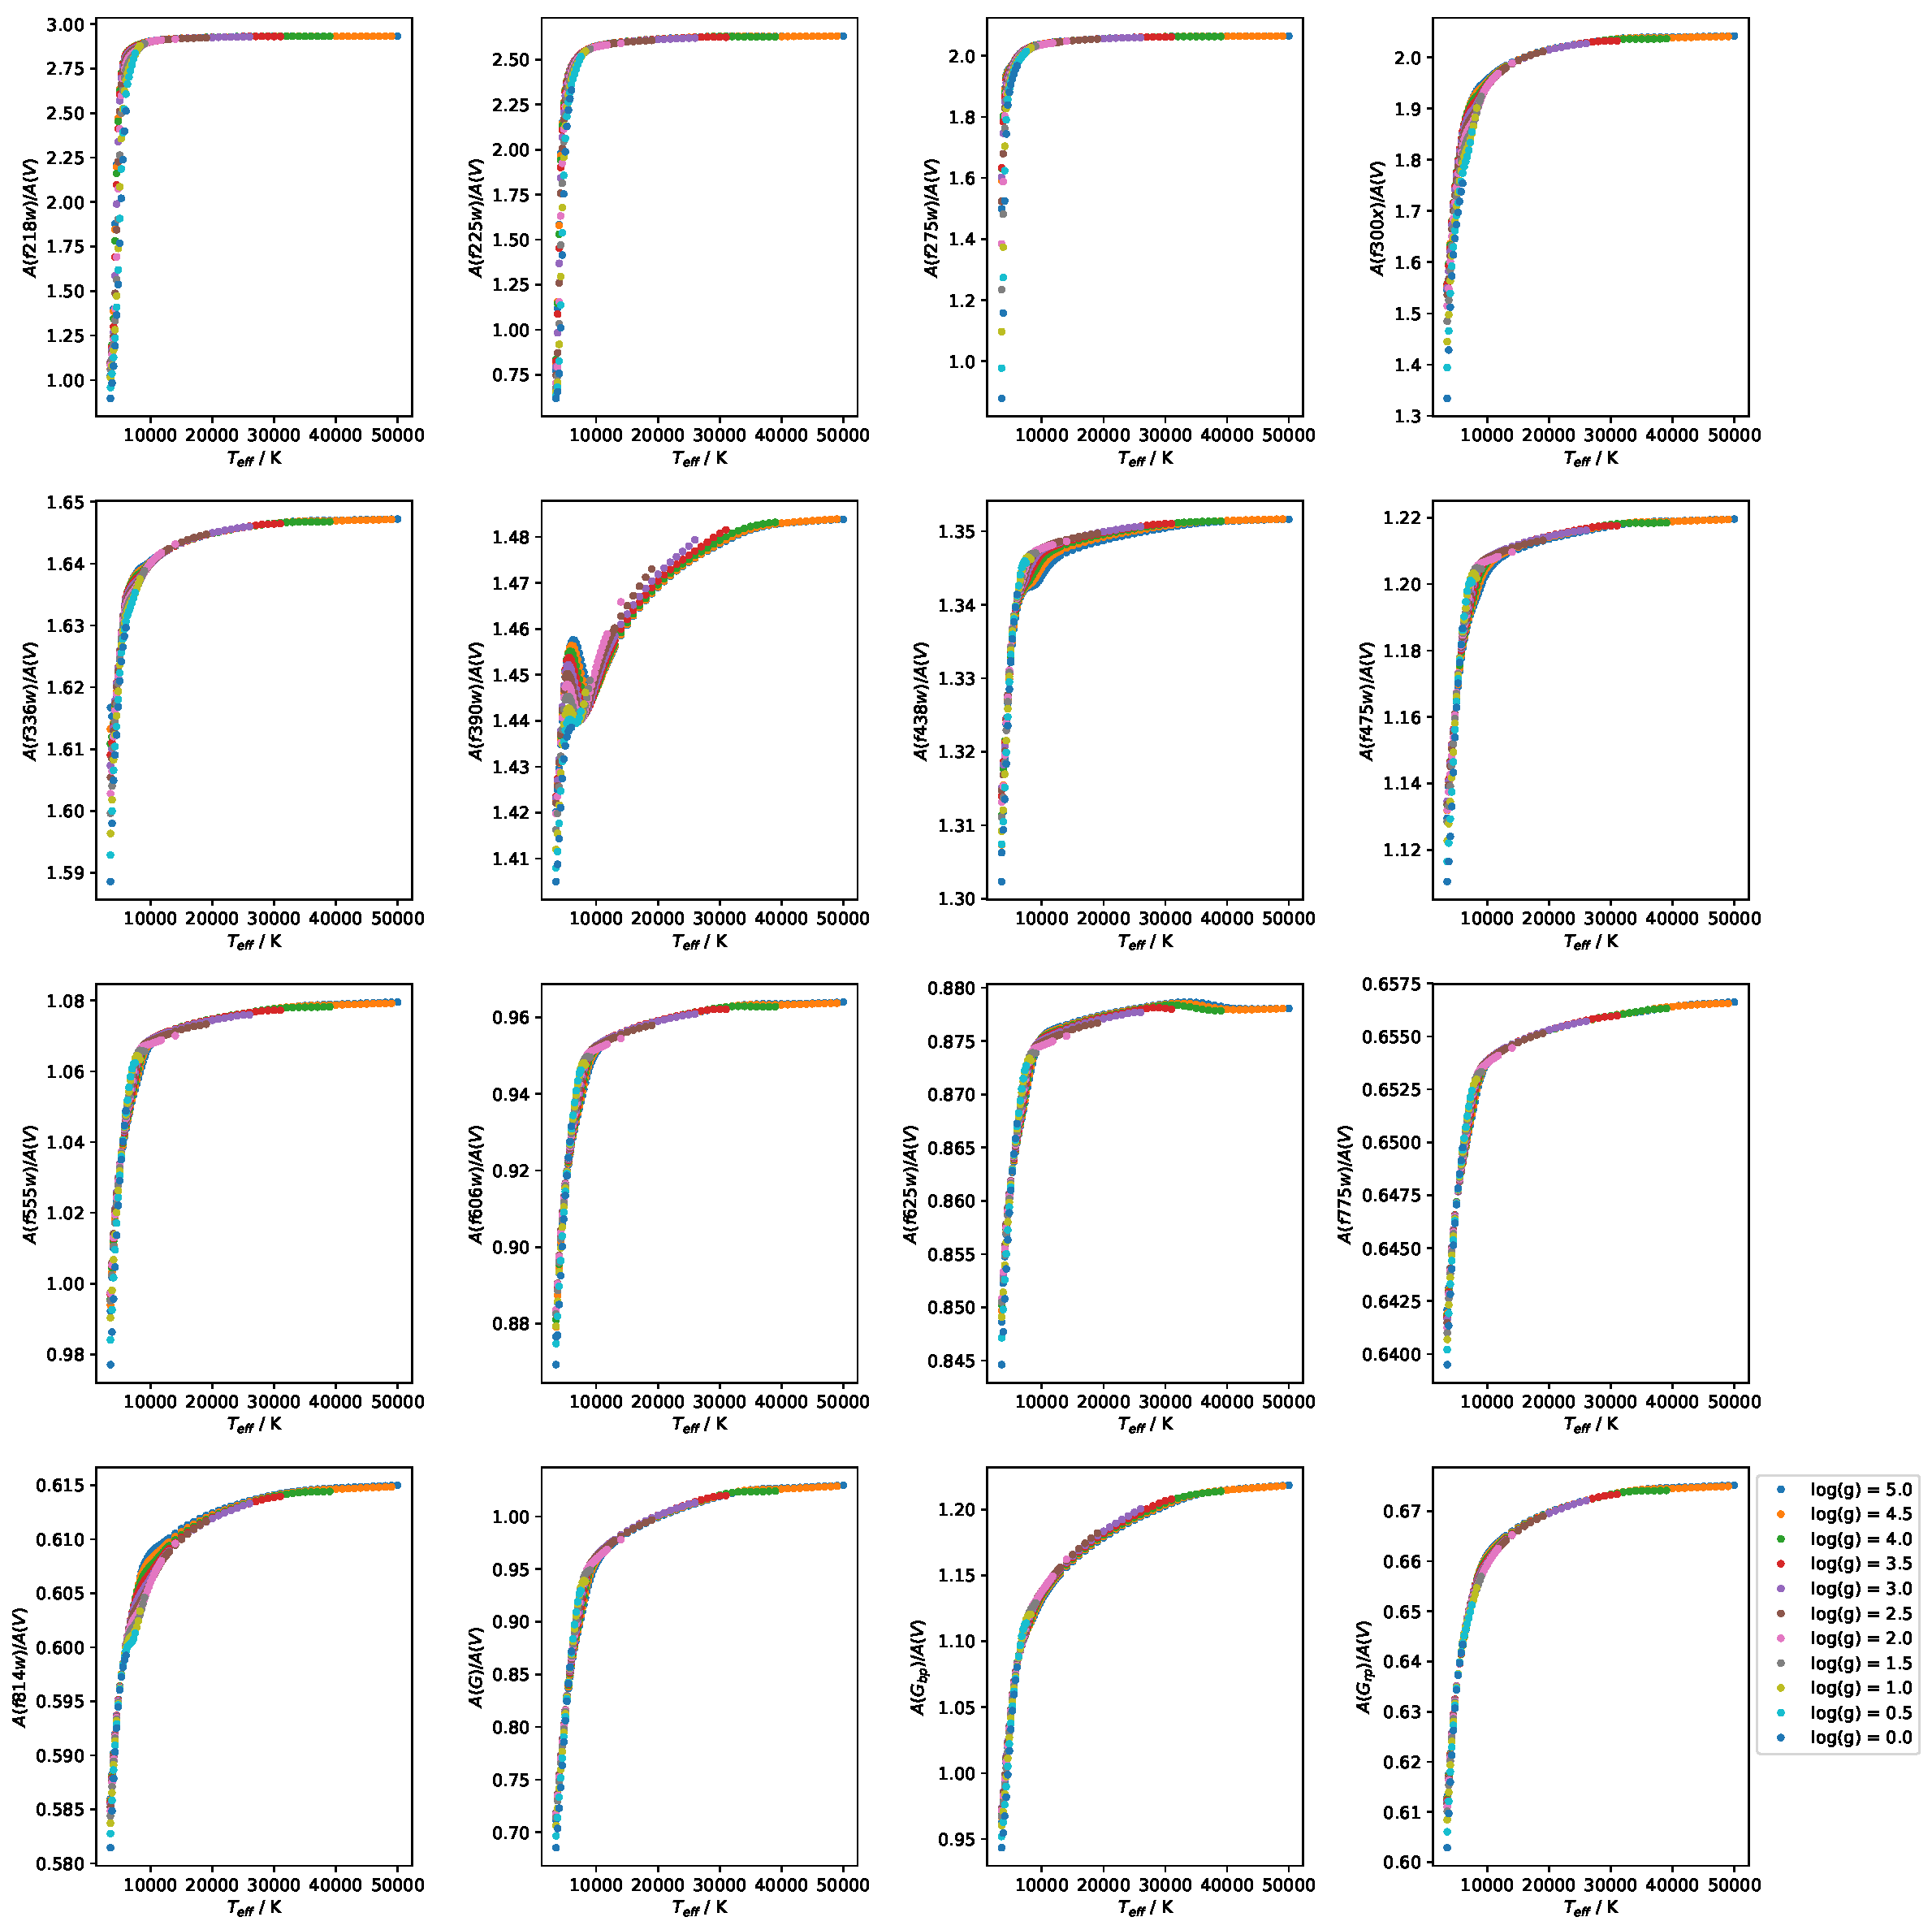
\includegraphics[scale=0.3]{../just_full_data/comb/AHub_FeHm2p0_just_Teff_fit_plot_dots.pdf}
\caption{WFC3 and Gaia filter $A_{X}/A_{V}$ data for [Fe/H] = -2, plotted against effective temperature, with each colour of dots representing a different value of log($g$).}
\label{comb Ax/Av data FeH=-2}
\end{center}
\end{figure}

\begin{figure}[h]
\begin{center}
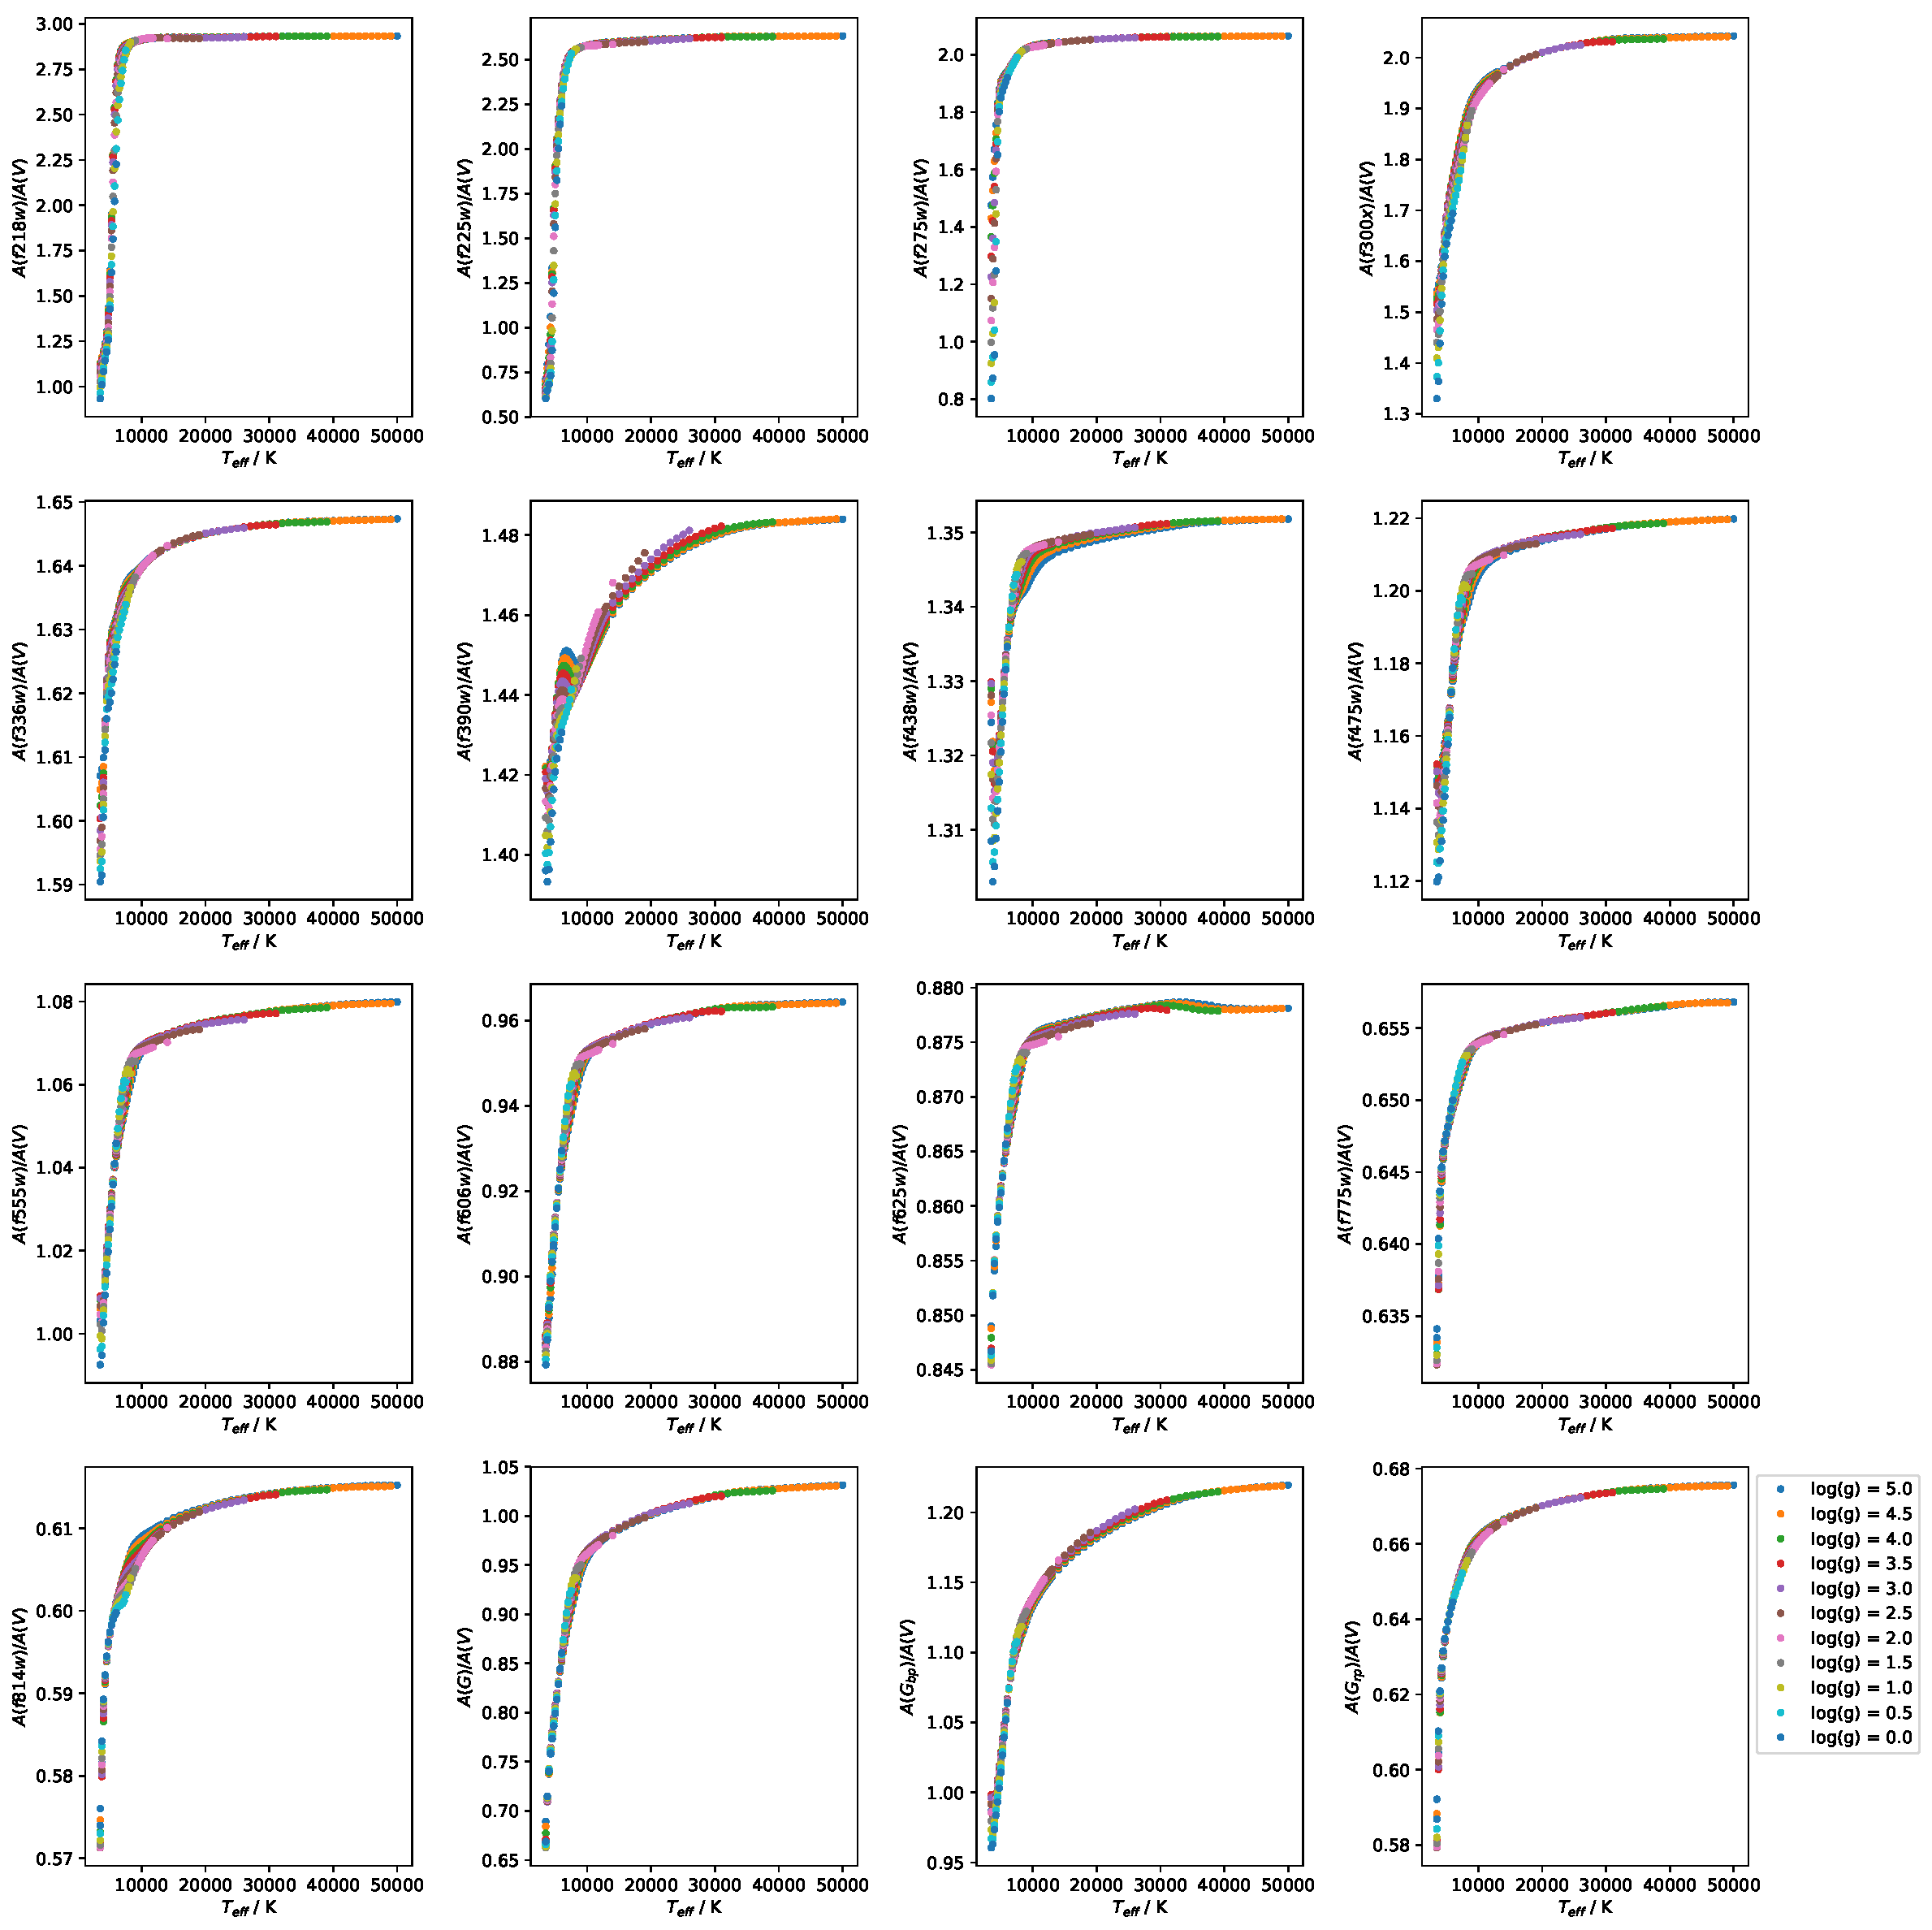
\includegraphics[scale=0.3]{../just_full_data/comb/AHub_FeH0p0_just_Teff_fit_plot_dots.pdf}
\caption{WFC3 and Gaia filter $A_{X}/A_{V}$ data for [Fe/H] = 0.5, plotted against effective temperature, with each colour of dots representing a different value of log($g$), showing the prominent presence of the tail-flick phenomenon in some filters.}
\label{comb Ax/Av data FeH=0}
\end{center}
\end{figure}

When calculating the bolometric corrections, the reference values taken by the parameters for Vega were:

\begin{enumerate}
\item $m_{X}^{0} = 0.03$ for the Gaia filters
\item $m_{X}^{0} = 0.00$ for the Hubble WFC3 filters
\end{enumerate}

together with $M_{\textnormal{bol},\odot} = 4.75$. The Vega model used in this project assumed $T_{\textnormal{eff}} = 9550$K and $\log(g) = 3.95$. The mean extinction law from \cite{1989ApJ...345..245C}, as shown in Equation \ref{CCM_general}, with its different wavelength regimes for $a(x)$ and $b(x)$, was used with the $A_{V}$ calibration values to simulate the extinction parameter in Equation \ref{BC_extinc}. $R_{V}$ was set to a value of 3.1, the standard value for the diffuse interstellar medium. The integration was carried out by iteratively adding the integrand results at regular small wavelength intervals. The non-zero calibration value of $A_{V} = 1$ was chosen, as this allows for significant changes in $A_{X}/A_{V}$ from Equation (\ref{BCs_diff}), while also being close enough to zero to avoid significant changes in $A_{X}/A_{V}$ due to the Forbes effect \citep{2008PASP..120..583G}.\\*

To generate extinction-coefficient ratios $A_{X}/A_{V}$ from the bolometric correction data, Equation \ref{BCs_diff} was used to calculate the differences between the BC($A_{V} = 0$) and BC($A_{V} = 1$) datasets and thereby give a single dataset of mean $A_{X}/A_{V}$ values (\cite{2008PASP..120..583G},\cite{2014MNRAS.444..392C}).

\begin{figure}[h]
\begin{center}
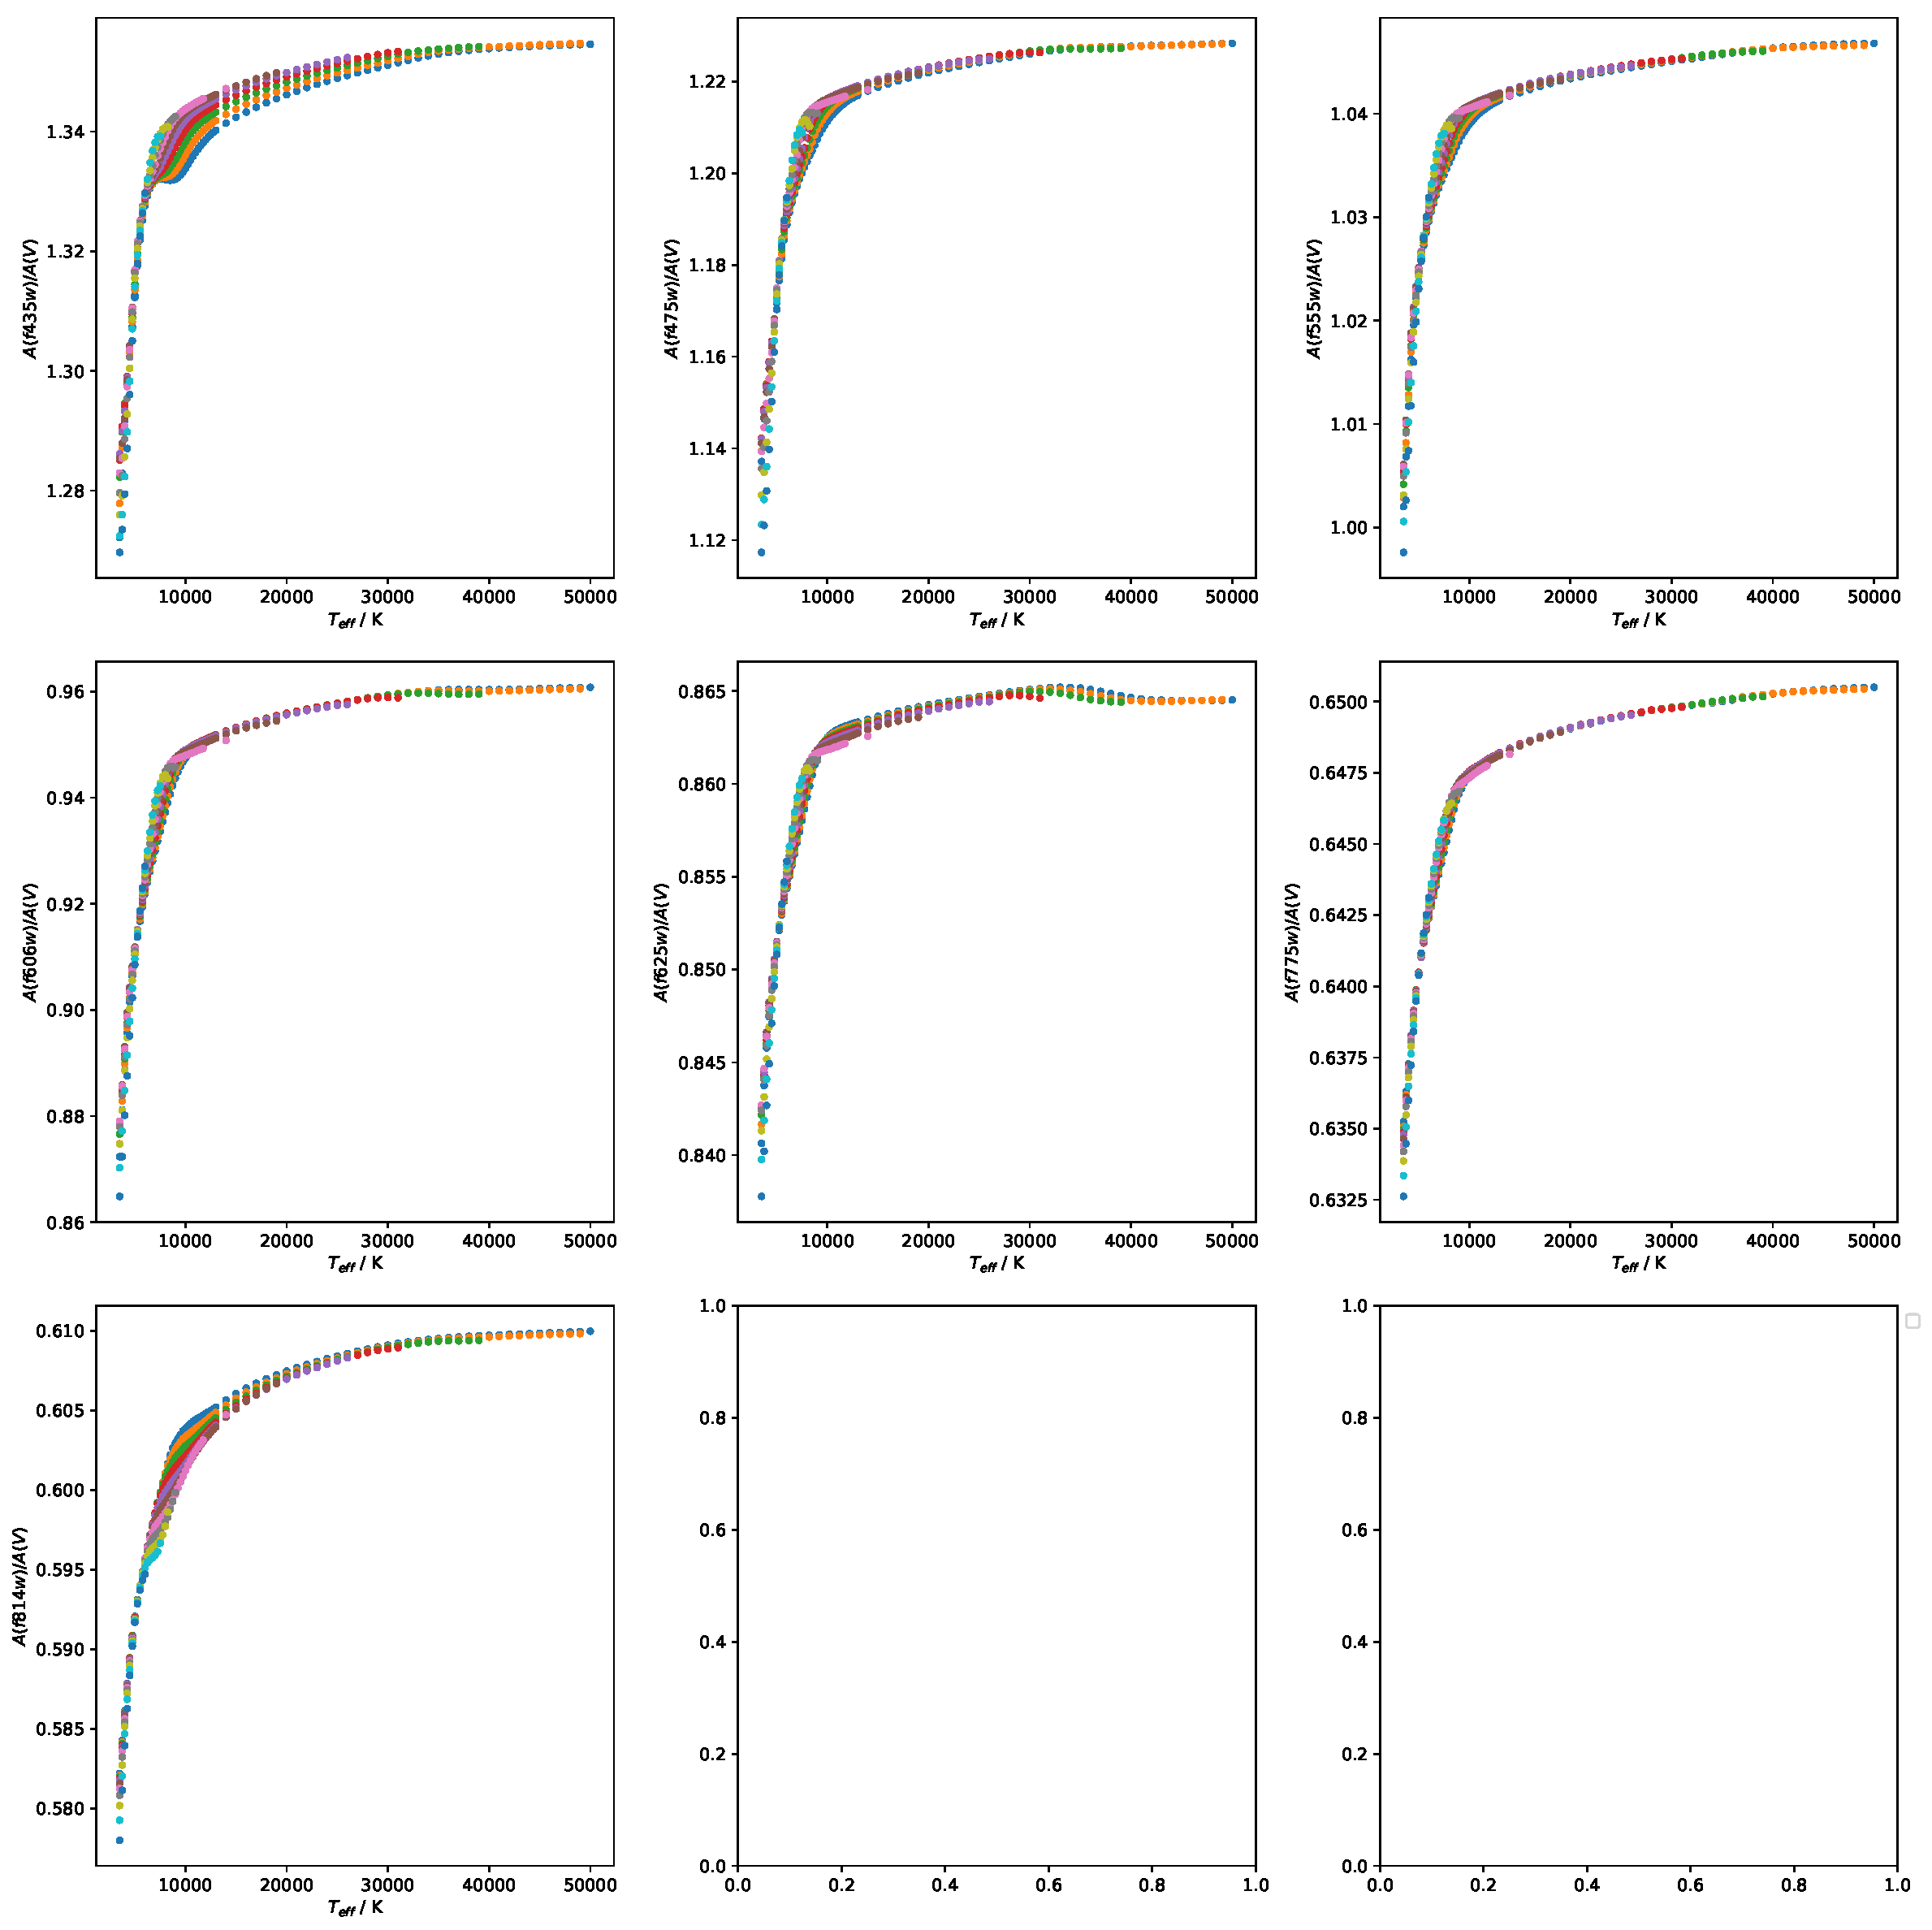
\includegraphics[scale=0.3]{../just_full_data/ACS/AHub_FeHm2p0_just_Teff_fit_plot_dots.pdf}
\caption{ACS filter $A_{X}/A_{V}$ data for [Fe/H] = -2, plotted against effective temperature, with each colour of dots representing a different value of log($g$).}
\label{acs Ax/Av data FeH=-2}
\end{center}
\end{figure}

\begin{figure}[h]
\begin{center}
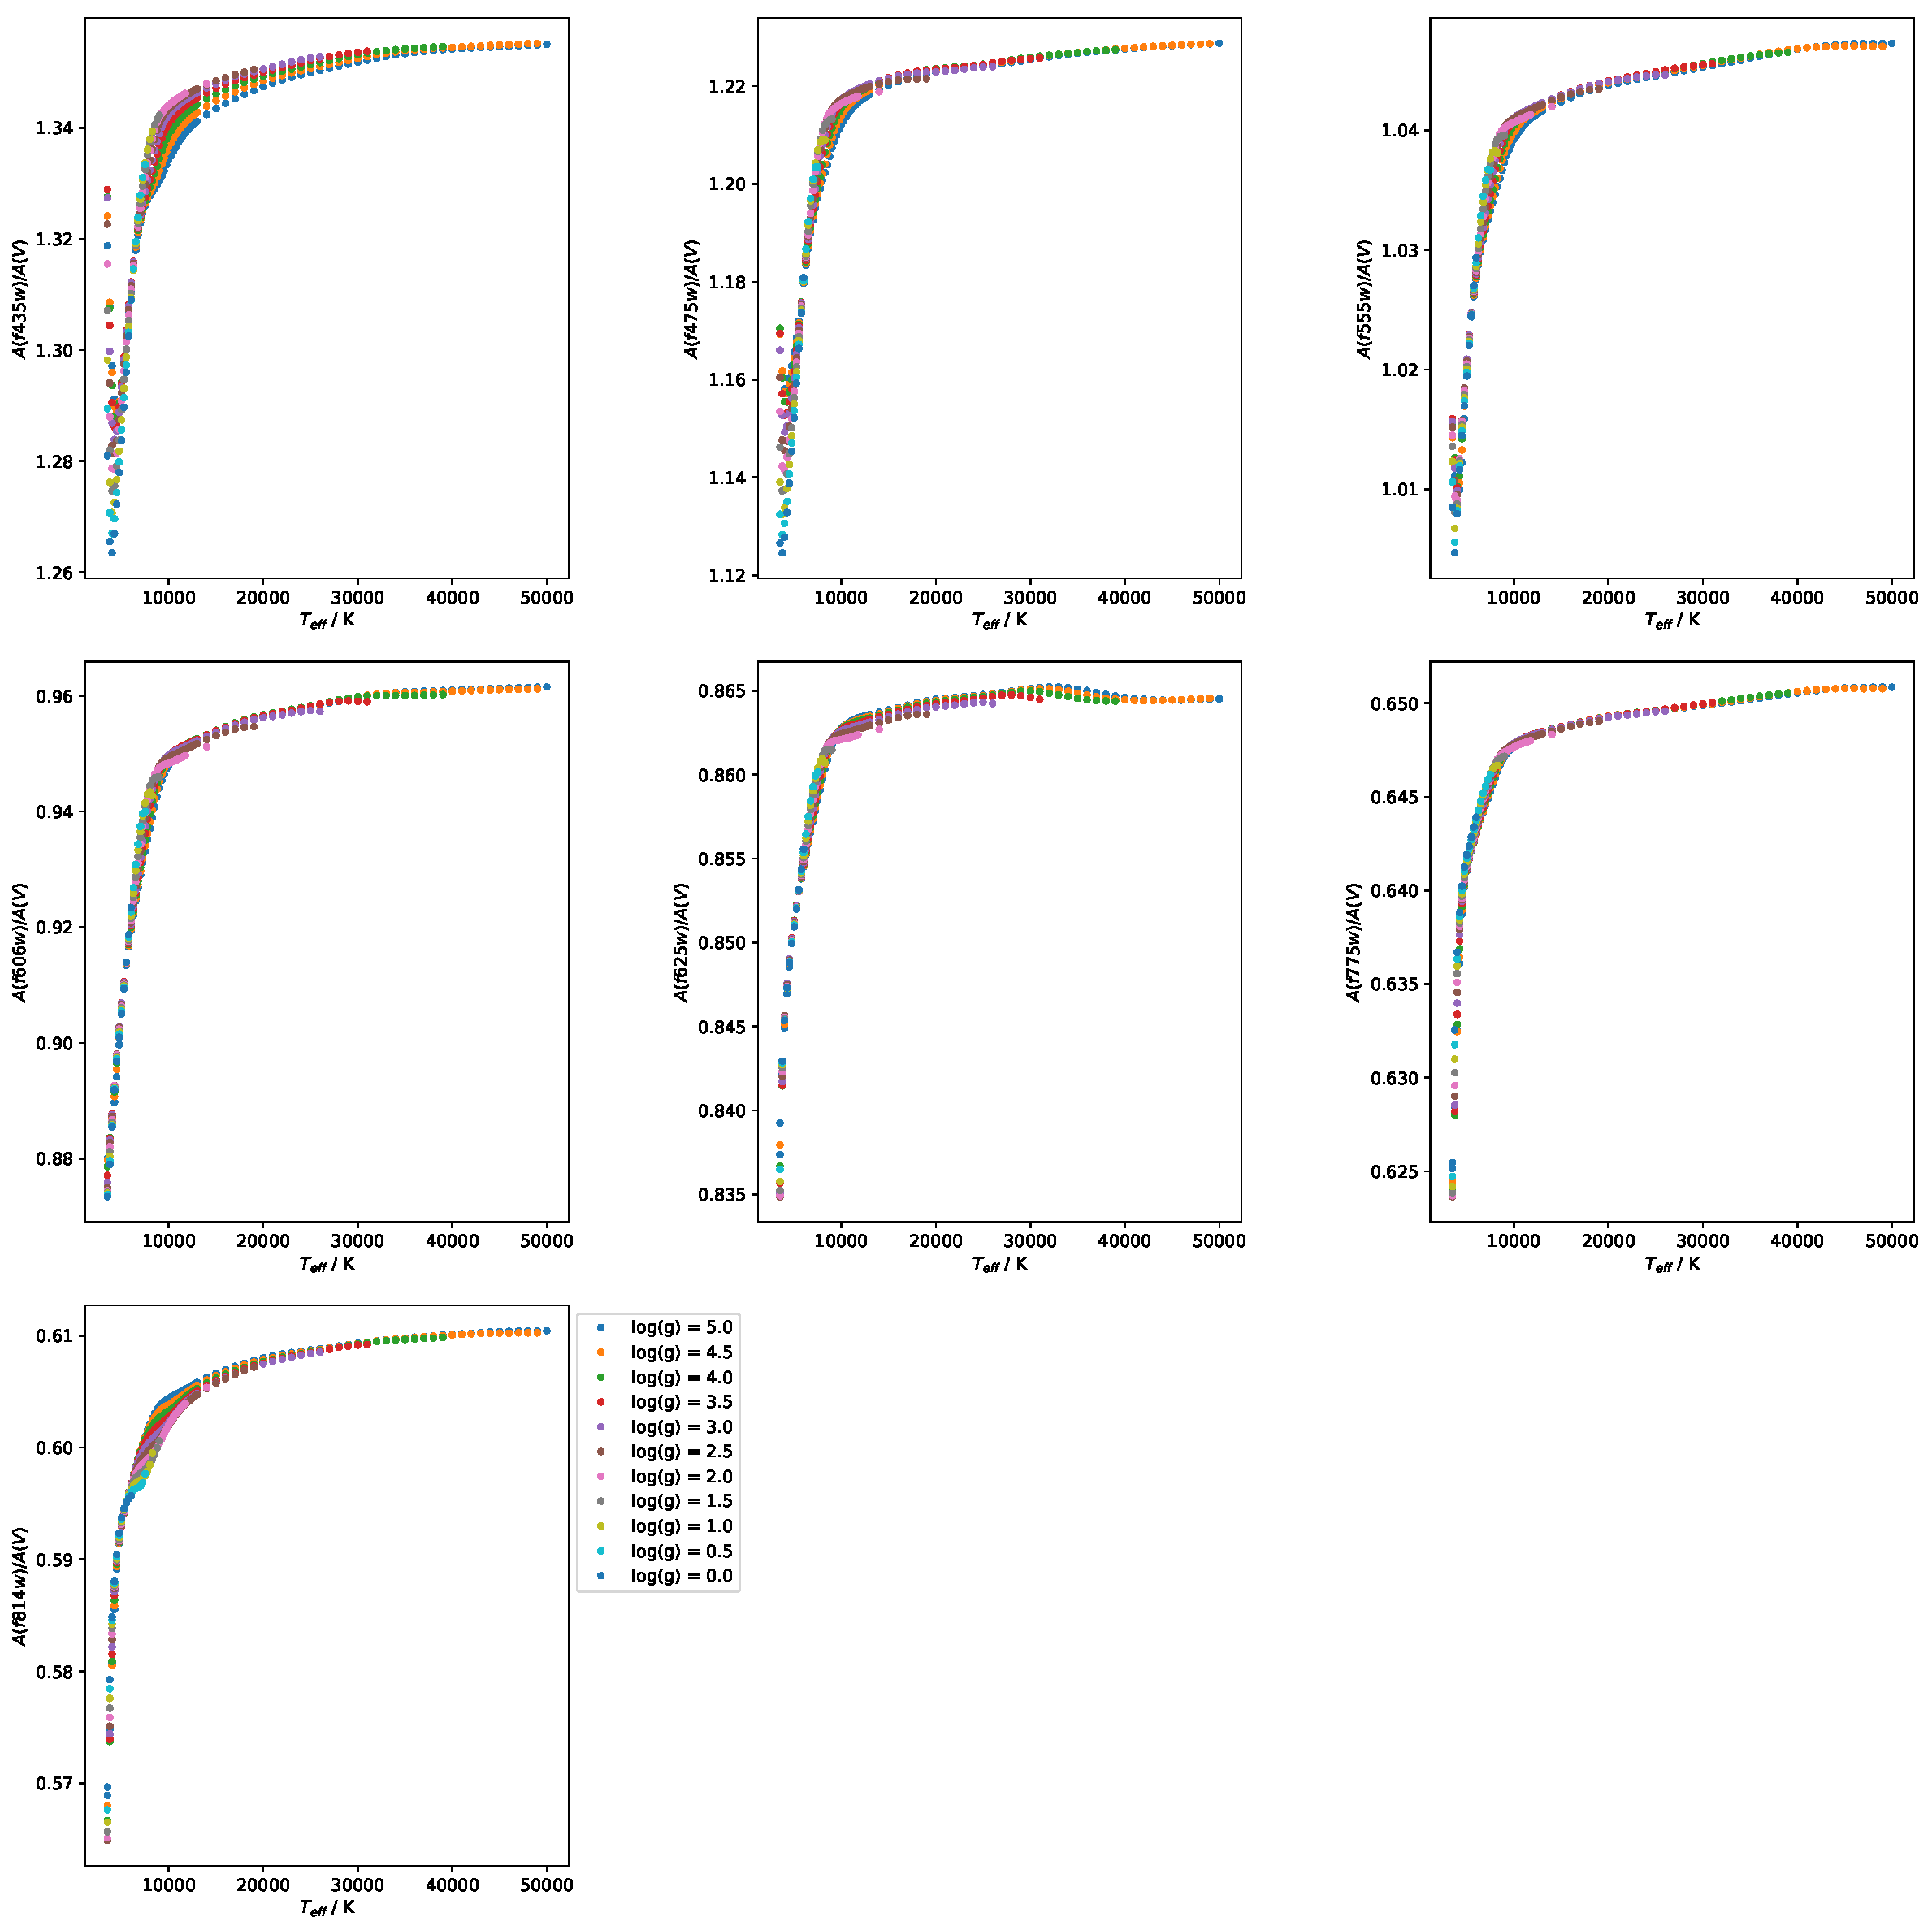
\includegraphics[scale=0.3]{../just_full_data/ACS/AHub_FeH0p5_just_Teff_fit_plot_dots.pdf}
\caption{ACS filter $A_{X}/A_{V}$ data for [Fe/H] = 0.5, plotted against effective temperature, with each colour of dots representing a different value of log($g$), showing the prominent presence of the tail-flick phenomenon in some filters.}
\label{acs Ax/Av data FeH=0}
\end{center}
\end{figure}

As can be seen in the data displayed in Figures \ref{comb Ax/Av data FeH=-2}-\ref{acs Ax/Av data FeH=0}, in almost all of the filters studied in this project, the longer the central wavelength of a given filter throughput, the smaller the average value of $A_{X}/A_{V}$, independent of all other parameters. This conforms with the expectation resulting from the fact that the physical mechanisms causing extinction in the ISM preferential affect photons with shorter wavelengths.\\*

Above $T_{\textnormal{eff}} \approx$ 12000-15000 K, the values of $A_{X}/A_{V}$ are approaching a constant value as a function of all three input parameters. This is reflected in the choice of decay functions as the fitting functions for the data. This region of parameter space will be referred to henceforth as the ``high-$T_{\textnormal{eff}}$ extinction plateau region'' or simply ``plateau''.\\*

\section{Finding \& fitting functions} \label{find_fit}
A property found in the data for some filters, more pronounced at higher metallicity but with a possible slight dependence on surface gravity, is the tendency of the gradient of $A_{X}/A_{V}$ with increasing $T_{\textnormal{eff}}$ to become significantly less positive at the lowest temperatures in the data, typically 4000K and below. The spread in $A_{X}/A_{V}$ values for different log($g$) is typically about 0.2-04, with a linear progression from log($g$) = 5.0 at the lowest end to log($g$) = 0.0 at the highest. In some filters, at the highest metallicity employed ([Fe/H] = 0.5), this phenomenon causes the gradient to invert and become significantly negative, reversing the trend everywhere else in the data, including for the same filters at lower metallicity. Due to the shape of the resulting point-to-point line in these axes, it has been dubbed the ``tail-flick'' phenomenon. This was ignored as an artefact from the numerical integration required for Equation \ref{BC_extinc}. This was due to the physical infeasibility of a cooler star experiencing a higher extinction $A_{X}$ for a globally-constant $A_{V}$ value and metallicity, as was assumed for data in each BC table. In the relevant filters, only effective temperatures above those affected by the gradient inversion was used for fitting.\\*

In order to find usable functions without running into issues with degeneracy between coefficients, the three input stellar parameters prioritising which parameters to model first, before expanding the function to include parts modelling the impact of other parameters and their associated coefficients. Too many coefficients created errors that were significantly greater in degenerate coefficients than in non-degenerate ones. This would obscure any useful information about the validity of the function form.\\*

The bolometric flux of a black body can be calculated as the total area under the curve described by the Planck function per unit wavelength/frequency as a function of wavelength/frequency. Since stellar emission spectra can be reasonably approximated by a black body emission with absorption lines, it can be seen from Equation\ref{Teff_def} that the greatest effect on stellar spectra, and therefore on the extinction coefficient, will come from effective temperature. Therefore, the initial functions to be fitted were simple analytical functions of $T_{\textnormal{eff}}$ only:

\begin{equation}
A_{\textnormal{pow}} (T_{\textnormal{eff}}) = a (T_{4})^{b} + c
\label{Teff_pow}
\end{equation}

\begin{equation}
A_{\textnormal{exp}} (T_{\textnormal{eff}}) = a \exp(b T_{4}) + c
\label{Teff_exp}
\end{equation}

where $T_{4} = 10^{-4} \times T_{\textnormal{eff}}$. The fitting operation was carried out on the data for solar metallicity ([Fe/H] = 0.0) and, because it gave the greatest number of $T_{\textnormal{eff}}$ data points, log($g$) = 5. This dataset will be referred to as the basic fitting data (BFD).\\*

For the data in the Gaia filters, the opportunity was taken to compare the model for $R_{X}$ and coefficients detailed for these filters by \cite{2018MNRAS.479L.102C}. To apply their model to the extinction ratios used for this project, the definition of $R_{X}$ was used to construct the following equation:

\begin{equation}
\frac{A_{X}}{A_{V}} = \frac{R_{X}}{R_{V}} = \frac{R_{X}}{3.1}
\label{convert_Rx_to_Ax}
\end{equation}

There were filters whose BFD could not support an accurate fit or maintain the desired accuracy across all combinations of log($g$) and [Fe/H] using $A_{\textnormal{pow}}$ or $A_{\textnormal{exp}}$. For these filters, more intricate functions were sought, including functions with explicit dependences on $g$ and [Fe/H]. Several unsuccessful approaches were made before an acceptable function was found for each filter.
%These included:

%\begin{itemize}
%\item Using a polynomial fit for the BFD, for filter which could not be accurately described in the BFD in the first instance.
%\item Fitting all the data in the ****parameter space in two steps, by fitting the residuals from the $A_{\textnormal{pow}}$ and $A_{\textnormal{exp}}$ fits to a new function with explicit variations in [Fe/H] and log($g$). The ****functions included second fittings of $A_{\textnormal{pow}}$ and $A_{\textnormal{exp}}$, damped-oscillator functions and oscillating power-law functions, among others. When fitted to the residuals, this meant an oscillation with amplitude decaying with increasing $T_{\textnormal{eff}}$
%\end{itemize}

The most successful approach was plotting all the available data for each filter, in multiple 2D and 3D axes, and analysing it visually. The trends seen in the data were transcribed to find not only an overarching function template, akin to the status of $A_{\textnormal{pow}}$ and $A_{\textnormal{exp}}$, but also smaller mathematical constructs within the template, such as describing a decay coefficient in terms of log($g$) and [Fe/H]. The details of the final form of the template as a function of each stellar parameter were deduced by fitting a logistic function of $T_{\textnormal{eff}}$ to the $A_{X}/A_{V}$ data for each ([Fe/H],log($g$)) combination. This was decided on the basis that $A_{\textnormal{exp}}$ had been superior to $A_{\textnormal{pow}}$ in describing the data for all relevant filters and because, for these filters, the low-$T_{\textnormal{eff}}$ change in gradient appeared to be more significant than for others and the gradient was not inverted, as can be seen in Figures \ref{comb Ax/Av data FeH=0}-\ref{acs Ax/Av data FeH=-2}. This is still the case, even after accounting for the difference in $A_{X}/A_{V}$ scale between filters. In particular, the $T_{\textnormal{eff}}$ gradient prior to the plateau appears to lead to an asymptote at lower, but still physically-viable, temperatures. This issue is resolved by the logistic function's property of converging to a constant value for both very high and low values of the input variable. 

For a general logistic function in $T_{\textnormal{eff}}$, there are four principle parameters:
\begin{itemize}
\item The global maximum value, denoted in this case by $A_{max}$;
\item The global minimum value, $A_{min}$;
\item The exponential decay coefficient, $k$;
\item The $T_{\textnormal{eff}}$-coordinate of the sigmoid midpoint, in this case $T_{\textnormal{0}}$.
\end{itemize}

It was confirmed that this new function could describe each scenario accurately enough for further analysis. The resulting coefficients were tabulated and analysed for trends and, if found, the nature of those trends. This allowed for the incremental construction of sub-functions of log($g$) and [Fe/H], making the overall function, $A_{logis}$, sensitive to all three input stellar atmosphere parameters, with effective temperature having the greatest effect and the relative effects of the other parameters dependent on the best-fit values of the relevant coefficients.\\*

The sub-functions of log($g$) and [Fe/H], upon inspection of the coefficients for the $T_{\textnormal{eff}}$-only logistic function, were found to be simple functions of log($g$) and [Fe/H], independent of $T_{\textnormal{eff}}$ variations. This allowed for them to be used as the definitions of $T_{0}$ and $k$, as shown in Equations \ref{T0_eq} and \ref{decay_const_eq}, respectively.

\begin{align}
T_{\textnormal{0}} &= a\log(g) + b\left(\frac{\left[\textnormal{Fe/H}\right]}{\left|\left[\textnormal{Fe/H}\right]\right|^{1/2}}\right) + c \label{T0_eq}\\
k &= d\log(g) + e\left[\textnormal{Fe/H}\right] + f \label{decay_const_eq}\\
A_{logis}(T_{\textnormal{eff}},g,\left[\textnormal{Fe/H}\right]) &= \frac{(A_{max}-A_{min})}{( 1 + \exp{(-10^{-4} k(T_{\textnormal{eff}}-T_{\textnormal{0}})) ) )}} + A_{min} \label{A_logis_UV}
\end{align}

The final form was then subjected to a final fit on the entire $A_{X}/A_{V}$ dataset, covering the entire ($T_{\textnormal{eff}}$,  log($g$), [Fe/H]) parameter space available. $A_{logis}$ was able to accurately reproduce the behaviour of almost the entire dataset. The details are given in Section \ref{coef_models}.\\*

\section{Isochrone data fitting}
To obtain isochrones from the BaSTI online database, the desired age range, initial metallicity and filter system must be specified. Therefore, the values of these quantities are shared by all stellar objects. For the stages in stellar evolution prior to the main-sequence turn-off, any changes in atmospheric metallicity are insignificant, due to the factors discussed in Section \ref{stel_evol}.\\*

The output from the BaSTI database for each model stellar object gives the model's initial mass and current mass (i.e. after a time equal to the isochrone age), together with the logarithms of the stellar luminosity in solar units ($\log(L/L_{\odot})$) and of the effective temperature in K ($\log(T_{\textnormal{eff}})$), followed by the absolute magnitudes (with zero extinction) of the object in each filter of the system. To derive the surface gravity $g$, we must combine Equation \ref{Teff_def}, to derive the stellar radius, and Equation \ref{gravity_def}. Equation \ref{gravity_LT_calc} shows the resultant definition of $g$:

\begin{equation}
\label{gravity_LT_calc}
g = \frac{4 \pi G M_{*} \sigma_{\textnormal{SB}} T_{\textnormal{eff}}^{4}}{L_{*}}
\end{equation}

After this had been completed, each object had a co-ordinate in ($T_{\textnormal{eff}}$, log($g$)) parameter space, plus the metallicity of the overall isochrone model. The filter magnitudes in the photometric data are the apparent magnitudes of the stars assigned to NGC 6793. Therefore, to match the quantities of the observational and isochrone datasets being compared, it was necessary to correct the observational data for distance and add extinction to the isochrones. This is that standard procedure used when analysing observational data. Thus, we were comparing the $M_{\textnormal{ext},X}$ values for the isochrones and the observational data. The functions described in Section \ref{find_fit} were then applied to the dataset of stellar objects, producing values of $M_{\textnormal{ext},X}$ for each filter for all objects, as is the standard for analysing observational data with unknown extinction coefficients.

\begin{table}
\begin{center}
\begin{tabular}{ccccc}
\hline
Isochrone & $T_{\textnormal{eff}}$ & $T_{\textnormal{eff}}$ & $\log(g)$ & $\log(g)$ \\
(Age/Myr , [Fe/H]) & minimum & maximum & minimum & maximum \\
\hline
500,0.002 & 2870 & 9640 & 0.886 & 5.137 \\
1000,0.002 & 2824 & 8035 & 1.608 & 5.184 \\
5000,-1.049 & 3118 & 7112 & 0.456 & 5.318 \\
10000,-1.049 & 3086 & 6412 & 0.286 & 5.332 \\
\hline
\end{tabular}
\caption{Ranges of effective temperature and surface gravities in selected BaSTI isochrones}
\label{variable_ranges}
\end{center}
\end{table}

The errors in the parallax data for objects assigned to NGC 6793 were significant, particularly for stars in the lower main-sequence - understandably, since they are the faintest objects in the data and therefore are more difficult to track against the background light sources. This leads to errors in the predicted $M_{\textnormal{ext},X}$ magnitudes, which is calculated by rearranging Equation \ref{distance_modulus}. The significance of the parallax errors in the main sequence is such that, any differences between isochrones with similar parameters are rendered insignificant. This is the case irrespective of photometric errors in the observed fluxes from the photometric filters.\\*

Since the table for photometric fluxes did not include photometric errors, the parallax errors alone accounted for the total error in the calculated $M_{\textnormal{ext},X}$. Therefore, the errors on the flux measurements  were exactly equal in all filters for a given star. The errors on the ($G_{\textnormal{bp}}-G_{\textnormal{rp}}$) color index were calculated as standard, by adding the individual filter errors in quadrature, giving the color errors which were a factor of $\sqrt{2}$ greater than those for the individual filter fluxes.\\*

When comparing the two approaches to extinction, in order to test for any differences in projected isochrone age via the MSTO, a range of ages must be considered. A ``primary'' age was utilised as the true cluster isochrone age. This primary isochrone was subjected to both the function-based (FBEC) and standard extinction-coefficient approaches. Two isochrones with ages equidistant from the primary were subjected to the standard approach only. All four of the resulting $M_{\textnormal{ext},X}$ isochrones were plotted together in the four chosen CMD axes, together with the original (zero-extinction) isochrone for visual reference.\\*

This procedure was employed for two values of $A_{X}/A_{V}$ standard fixed extinction treatment. Both were extracted from the ATLAS9 data tables for a log($g$) value of 5.0 to represent a main-sequence star, highly desirable when comparing MSTO positions. The ATLAS9 metallicity chosen for calculating these $A_{X}/A_{V}$ values was that which best matched the metallicity of the isochrone to which the coefficient was applied. The ATLAS9 value will be denoted [Fe/H]$_{CM}$. The first value was equal to $(A_{X}/A_{V})_{plat} = (A_{X}/A_{V})(T_{\textnormal{eff}} = 50,000\textnormal{K},\log(g) = 5.0,\textnormal{[Fe/H]}_{CM})$, and the second was equal to $(A_{X}/A_{V})_{MS} = (A_{X}/A_{V})(T_{\textnormal{eff}} = 5,000\textnormal{K},\log(g) = 5.0,\textnormal{[Fe/H]}_{CM})$. This was done to reflect the fact that, on one hand, the assumption of a constant extinction coefficient is valid in the plateau region and, on the other, given the position of the MSTO in terms of stellar model $T_{\textnormal{eff}}$ values, it would be more prudent to ensure that the upper main sequences resulting from both approaches to extinction coincide in the CMD, making it easier to see any disagreements in the turn-off ages. For each of these plots, $A_{V}$ was fixed at a value of 1.0.\\*

Given the large number of filters studied in this project, four commonly-used CMD axes were selected to test for any effects of a function-derived $A_{X}$. Two of these are specific to the WFC3 system, with one CMD each for ACS and Gaia.

\section{Observational test case: NGC 6793}
To test the effects of the difference in treatment of $A_{X}/A{V}$ on observational data, both cases were employed to predict the isochrone parameters (age,[Fe/H] and $A_{V}$) of the open cluster NGC 6793.

NGC 6793 has little information available in the literature when compared to open clusters. Two observational studies have been published which give estimates for the properties of the cluster. Both sets of results are listed in Table \ref{NGC6793_obs}.

\begin{table}
\begin{center}
\begin{tabular}{ccc}
\hline
%\multirow{2}{*}{System} & \multirow{2}{*}{Filter} & \multirow{2}{*}{$A_{1}$ function} & \multicolumn{3}{c}{$A_{1}$ coefficients} \\ \cline{4-6}
%\textbf{Filter} \\
Cluster property & K05 & GC18 \\
\hline
Distance modulus / mag & 10.73 & 8.894 \\
-> distance / pc & 1400 & 601 \\
log(age / yr) & 8.64 & 8.78 \\
-> Age / Myr & 437 & 603 \\
$E(B-V)$ / mag & 0.17 & 0.272 \\
$[Fe/H]$ & ? & ? \\
Members & ? (> 3 ACSS-2.5) & 465 (271 with Gaia photometry) \\
\hline
\end{tabular}
\caption{Observational parameters for NGC 6793, according to \cite{2005A&A...438.1163K} (WEBDA archive page) and \cite{2018A&A...616A..10G}}
\label{NGC6793_obs}
\end{center}
\end{table}

The Gaia DR2 dataset for NGC 6793, containing the parallaxes and apparent magnitudes (in all three Gaia filters) for 338 objects identified as belonging to the cluster, was obtained. The number of objects is greater than the 271 photometric Gaia objects found by \cite{2018A&A...616A..10G}. In addition to this, there were significant variations in the observed parallaxes of individual stars, far beyond the maximum cluster radii expected (\cite{2006A&A...456..523S}). Some objects were even assigned negative parallax values, which are therefore mathematically impossible. Restrictions on the parallax measurements were implemented, by imposing a distance-based selection range centred at 600 pc, which was treated as the centre of the cluster, in line with the \cite{2018A&A...616A..10G} estimate in Table \ref{NGC6793_obs}. The range was decreased until the remaining sample size was approximately equal to 271. When this was implemented, the final sample of observational data for NGC 6793 contained 274 objects. Some of these objects still had parallax distances further from the cluster centre than would be expected for any star cluster. The size of the final dataset balanced the need for maintaining sufficient data points, to achieve a valid comparison to the previous studies of NGC 6793, and eliminating anomalous data.\\*

The isochrone fitting to the NGC 6793 was done by eye using a plot of the cluster's observed Gaia CMD, the position of each star corrected for its parallax distance. Using the values of $E(B-V)$ and age from \cite{2018A&A...616A..10G}, a standard-case isochrone was derived, again assuming a diffuse ISM (i.e., $R_{V} = 3.1$). The standard treatment was employed twice, creating a different isochrone each time. A coefficient calculated from $(A_{X}/A_{V})_{MS}$ was applied in one case and one calculated using $(A_{X}/A_{V})_{plat}$ in the other. The fitting process was carried out in sequential stages:

\begin{enumerate}
\item First, the upper main sequence of the FBEC isochrone was fitted to that of the standard-case isochrone by varying the value of $A_{V}$ used to calculate the final FBEC value for each stellar object.
\item Next, the age of the FBEC isochrone was varied to match the observed turn-off location in the NGC 6793 data as far as possible.
\item Finally, the FBEC isochrone metallicity was varied in an attempt match the observed lower main-sequence.
\end{enumerate}

The isochrone with the resulting parameters were then plotted alongside two standard-case isochrones, The resulting curves were compared to each other for accuracy with respect to the observational data.



\chapter{Results and discussion}
\section{Extinction coefficient models} \label{coef_models}

\begin{table}
\begin{center}
\begin{tabular}{cccccc}
\hline
%\multirow{2}{*}{System} & \multirow{2}{*}{Filter} & \multirow{2}{*}{$A_{1}$ function} & \multicolumn{3}{c}{$A_{1}$ coefficients} \\ \cline{4-6}
%\textbf{Filter} \\
System & Filter &  Function & & Coefficients & \\
 & & ($A_{\textnormal{pow}}$ or $A_{\textnormal{exp}}$) & $a$ & $b$ & $c$ \\
\hline

& F435W & pow & -0.0276$\pm$0.0061 & -0.967$\pm$0.1918 & 1.3613$\pm$0.005 \\
& F475W & pow & -0.0235$\pm$0.0042 & -1.2855$\pm$0.174 & 1.2323$\pm$0.0032 \\
& F555W & pow & -0.0089$\pm$0.0034 & -1.534$\pm$0.3895 & 1.0473$\pm$0.0026 \\
ACS & F606W & exp & -0.2295$\pm$0.0361 & -2.9413$\pm$0.3326 & 0.9591$\pm$0.0017 \\
& F625W & exp & -0.0741$\pm$0.0487 & -3.3839$\pm$1.4339 & 0.8647$\pm$0.0016 \\
& F775W & exp & -0.0695$\pm$0.0649 & -3.8286$\pm$2.0938 & 0.6497$\pm$0.0016 \\
& F814W & exp & -0.0909$\pm$0.0438 & -3.2279$\pm$1.0425 & 0.6086$\pm$0.0016 \\ \hline

%& F218W & R2fle & -232.4$\pm$48.1 & -(1.076$\pm$0.043)$\times 10^{-3}$ & 2.933$\pm$0.007 \\
%& F225W & R2fle & -128.5$\pm$13.8 & -(1.031$\pm$0.022)$\times 10^{-3}$ & 2.610$\pm$0.003 \\
%& F275W & R2fle & 0.9726$\pm$0.0581 & -(3.518$\pm$0.109)$\times 10^{-4}$ & 2.060$\pm$0.001 \\
%& F300X & R1fle & -(5.335$\pm$0.936)$\times 10^{5}$ & -1.664$\pm$0.021 & 2.052$\pm$0.001 \\

& F336W & pow & -0.0064$\pm$0.0028 & -1.8004$\pm$0.4633 & 1.6472$\pm$0.0022 \\
& F390W & exp & -0.0763$\pm$0.0061 & -0.7961$\pm$0.1602 & 1.486$\pm$0.0035 \\
& F438W & exp & -0.0839$\pm$0.0284 & -2.5967$\pm$0.6941 & 1.3507$\pm$0.0017 \\
& F475W & pow & -0.0224$\pm$0.0041 & -1.3107$\pm$0.1793 & 1.2233$\pm$0.0031 \\
WFC3 & F555W & exp & -0.2282$\pm$0.0396 & -3.0752$\pm$0.3704 & 1.0776$\pm$0.0017 \\
& F606W & exp & -0.2271$\pm$0.0368 & -2.9707$\pm$0.3438 & 0.9622$\pm$0.0017 \\
& F625W & pow & -0.0048$\pm$0.0028 & -1.8035$\pm$0.6184 & 0.879$\pm$0.0022 \\
& F775W & exp & -0.0713$\pm$0.0695 & -3.9365$\pm$2.1978 & 0.6558$\pm$0.0016 \\
& F814W & pow & -0.0058$\pm$0.0029 & -1.7434$\pm$0.5318 & 0.6149$\pm$0.0023 \\ \hline

& G & pow & -0.0952$\pm$0.0042 & -1.2853$\pm$0.043 & 1.044$\pm$0.0032 \\
Gaia & G\textsubscript{bp} & pow & -0.1258$\pm$0.0081 & -0.7984$\pm$0.0499 & 1.2562$\pm$0.0069 \\
& G\textsubscript{rp} & pow & -0.013$\pm$0.0031 & -1.6863$\pm$0.2444 & 0.6753$\pm$0.0023 \\ \hline

\end{tabular}
\caption{Coefficient values produced for each filter via $A_{\textnormal{exp}}$ or $A_{\textnormal{exp}}$ fitting, as appropriately labelled. Any filters missing from this table are those with data that could not be accurately fitted using either function.}
\label{simpfunc_coeffs_table}
\end{center}
\end{table}

The extinction-ratio data for all filters, with the exception of the four fully-UV filters in the WFC3 system, could be accurately modelled by the simplest functions trialled for fitting, $A_{\textnormal{pow}} (T_{\textnormal{eff}})$ or $A_{\textnormal{pow}} (T_{\textnormal{eff}})$.
\begin{table}
\begin{center}
\begin{tabular}{ccccc}
\hline

Filter &  Function & & Coefficients & \\
 & ($A_{\textnormal{pow}}$ or $A_{\textnormal{exp}}$) & $a$ & $b$ & $c$ \\
\hline
F218W & exp & -0.0763$\pm$0.0061 & -0.7961$\pm$0.1602 & 1.486$\pm$0.0035 \\
F225W & exp & -0.0839$\pm$0.0284 & -2.5967$\pm$0.6941 & 1.3507$\pm$0.0017 \\
F275W & pow & -0.0224$\pm$0.0041 & -1.3107$\pm$0.1793 & 1.2233$\pm$0.0031 \\
F300X & blah**** & -0.2282$\pm$0.0396 & -3.0752$\pm$0.3704 & 1.0776$\pm$0.0017 \\
\hline
\end{tabular}
\caption{Coefficient values for non-trivial functions produced for fitting to UV filter data.}
\label{UV_coeffs_table}
\end{center}
\end{table}

All the functions are consistent with the general trends predicted by the physics in stellar atmospheres, since the effective temperature has the greatest effect upon the value of $A_{X}/A_{V}$, with relatively minor differences due to 

The $(A_{X}/A_{V})$ data which underpinned this project was derived using the mean extinction laws prescribed in \cite{1989ApJ...345..245C}. These equations were derived by studying trends in 

\section{Effect on isochrones} \ref{result_CMDs}
Given the large number of filters studied in Section \ref{coef_models}, four commonly-used CMD axes were selected to test for any effects of a function-derived $A_{X}$. Two of these are specific to the WFC3 system, with one CMD each for ACS and Gaia.
\subsection{ACS} \label{ACS_isoc}

The CMD chosen for the ACS was the F435W-(F435W-F814W) axis combination. This CMD is useful as it pairs the bluest and reddest wide-field filters for the ACS in its colour index, which is the index most likely to distinguish between objects with a large range of effective temperatures, making it useful for modelling the main sequence and MSTO, the two most important CMD components for calculating cluster isochrone ages.

\begin{figure}[h]
\begin{center}
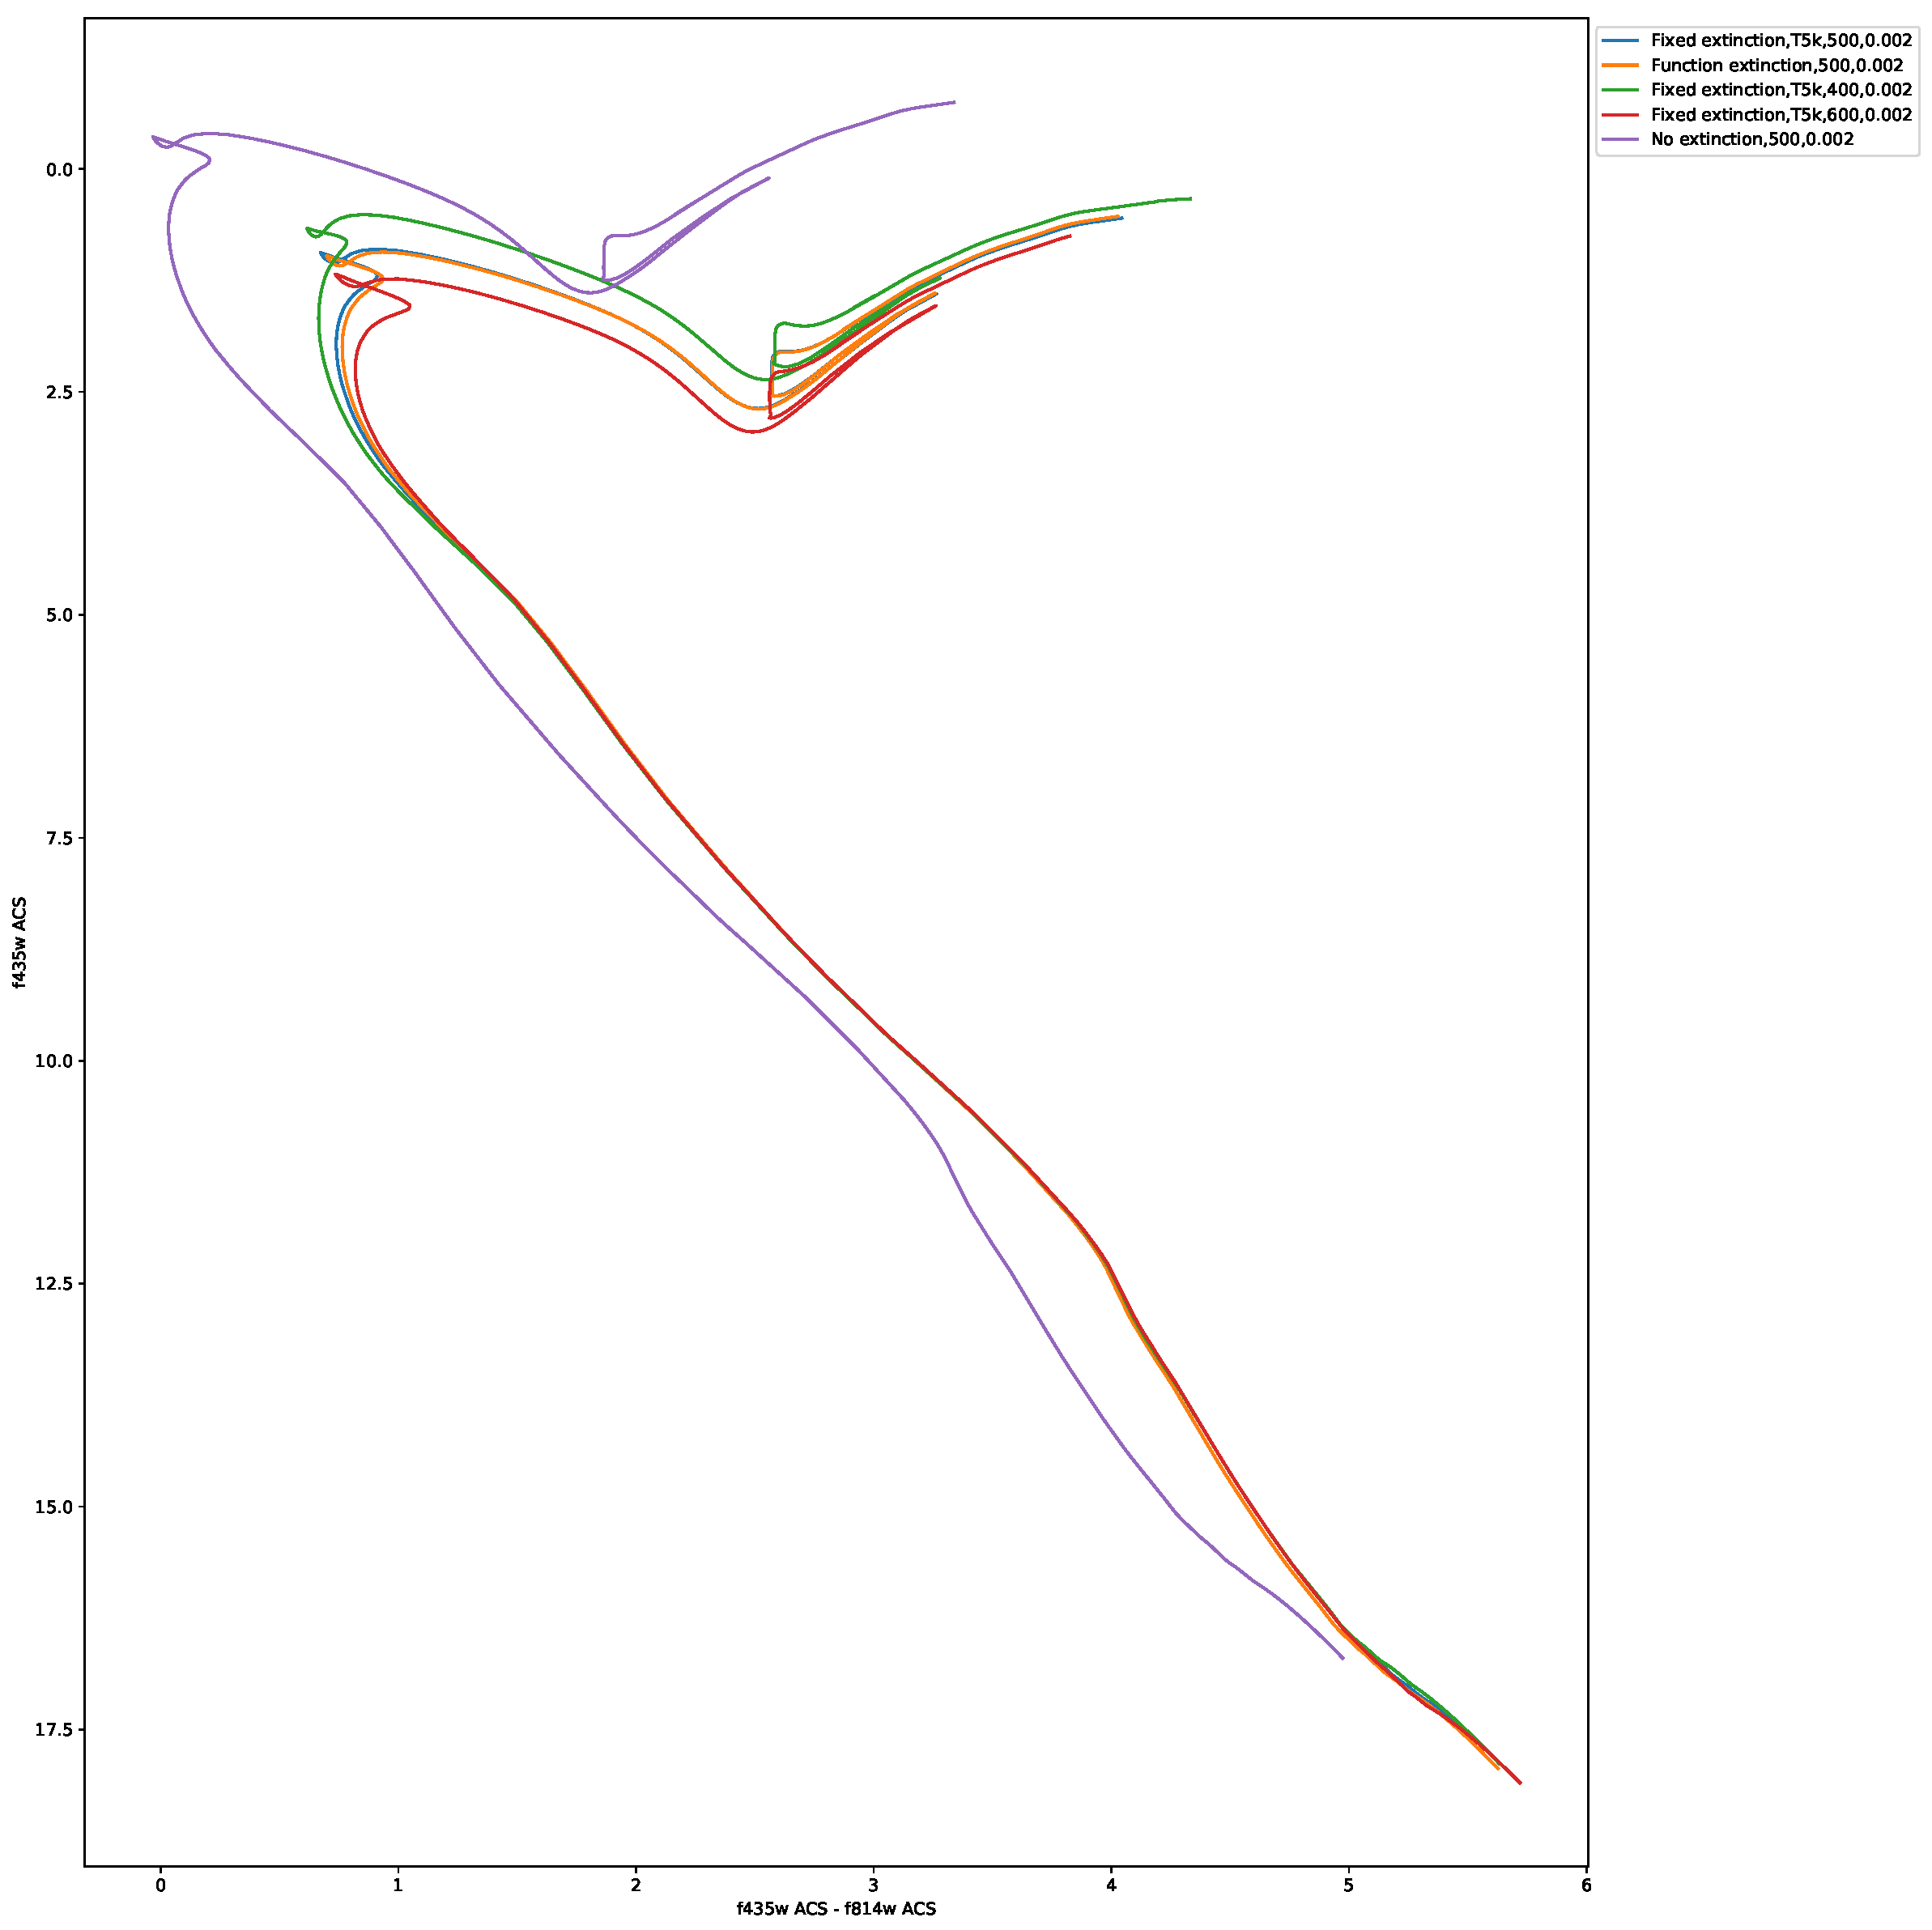
\includegraphics[scale=0.3]{../basti_isochrones_10_13Gyr/Extinction_T5k_FeH0fix_func_f435wACS_f435wACSmf814wACS_500_400_600_Myr_FeH_0p002_ref_noext_Av_1p0.pdf}
\caption{ACS F435W-(F435W-F814W) CMD with a fixed extinction coefficient equal to $(A_{X}/A_{V})_{MS}$ for each filter}
\label{acs_isoc_T5k}
\end{center}
\end{figure}

\begin{figure}[h]
\begin{center}
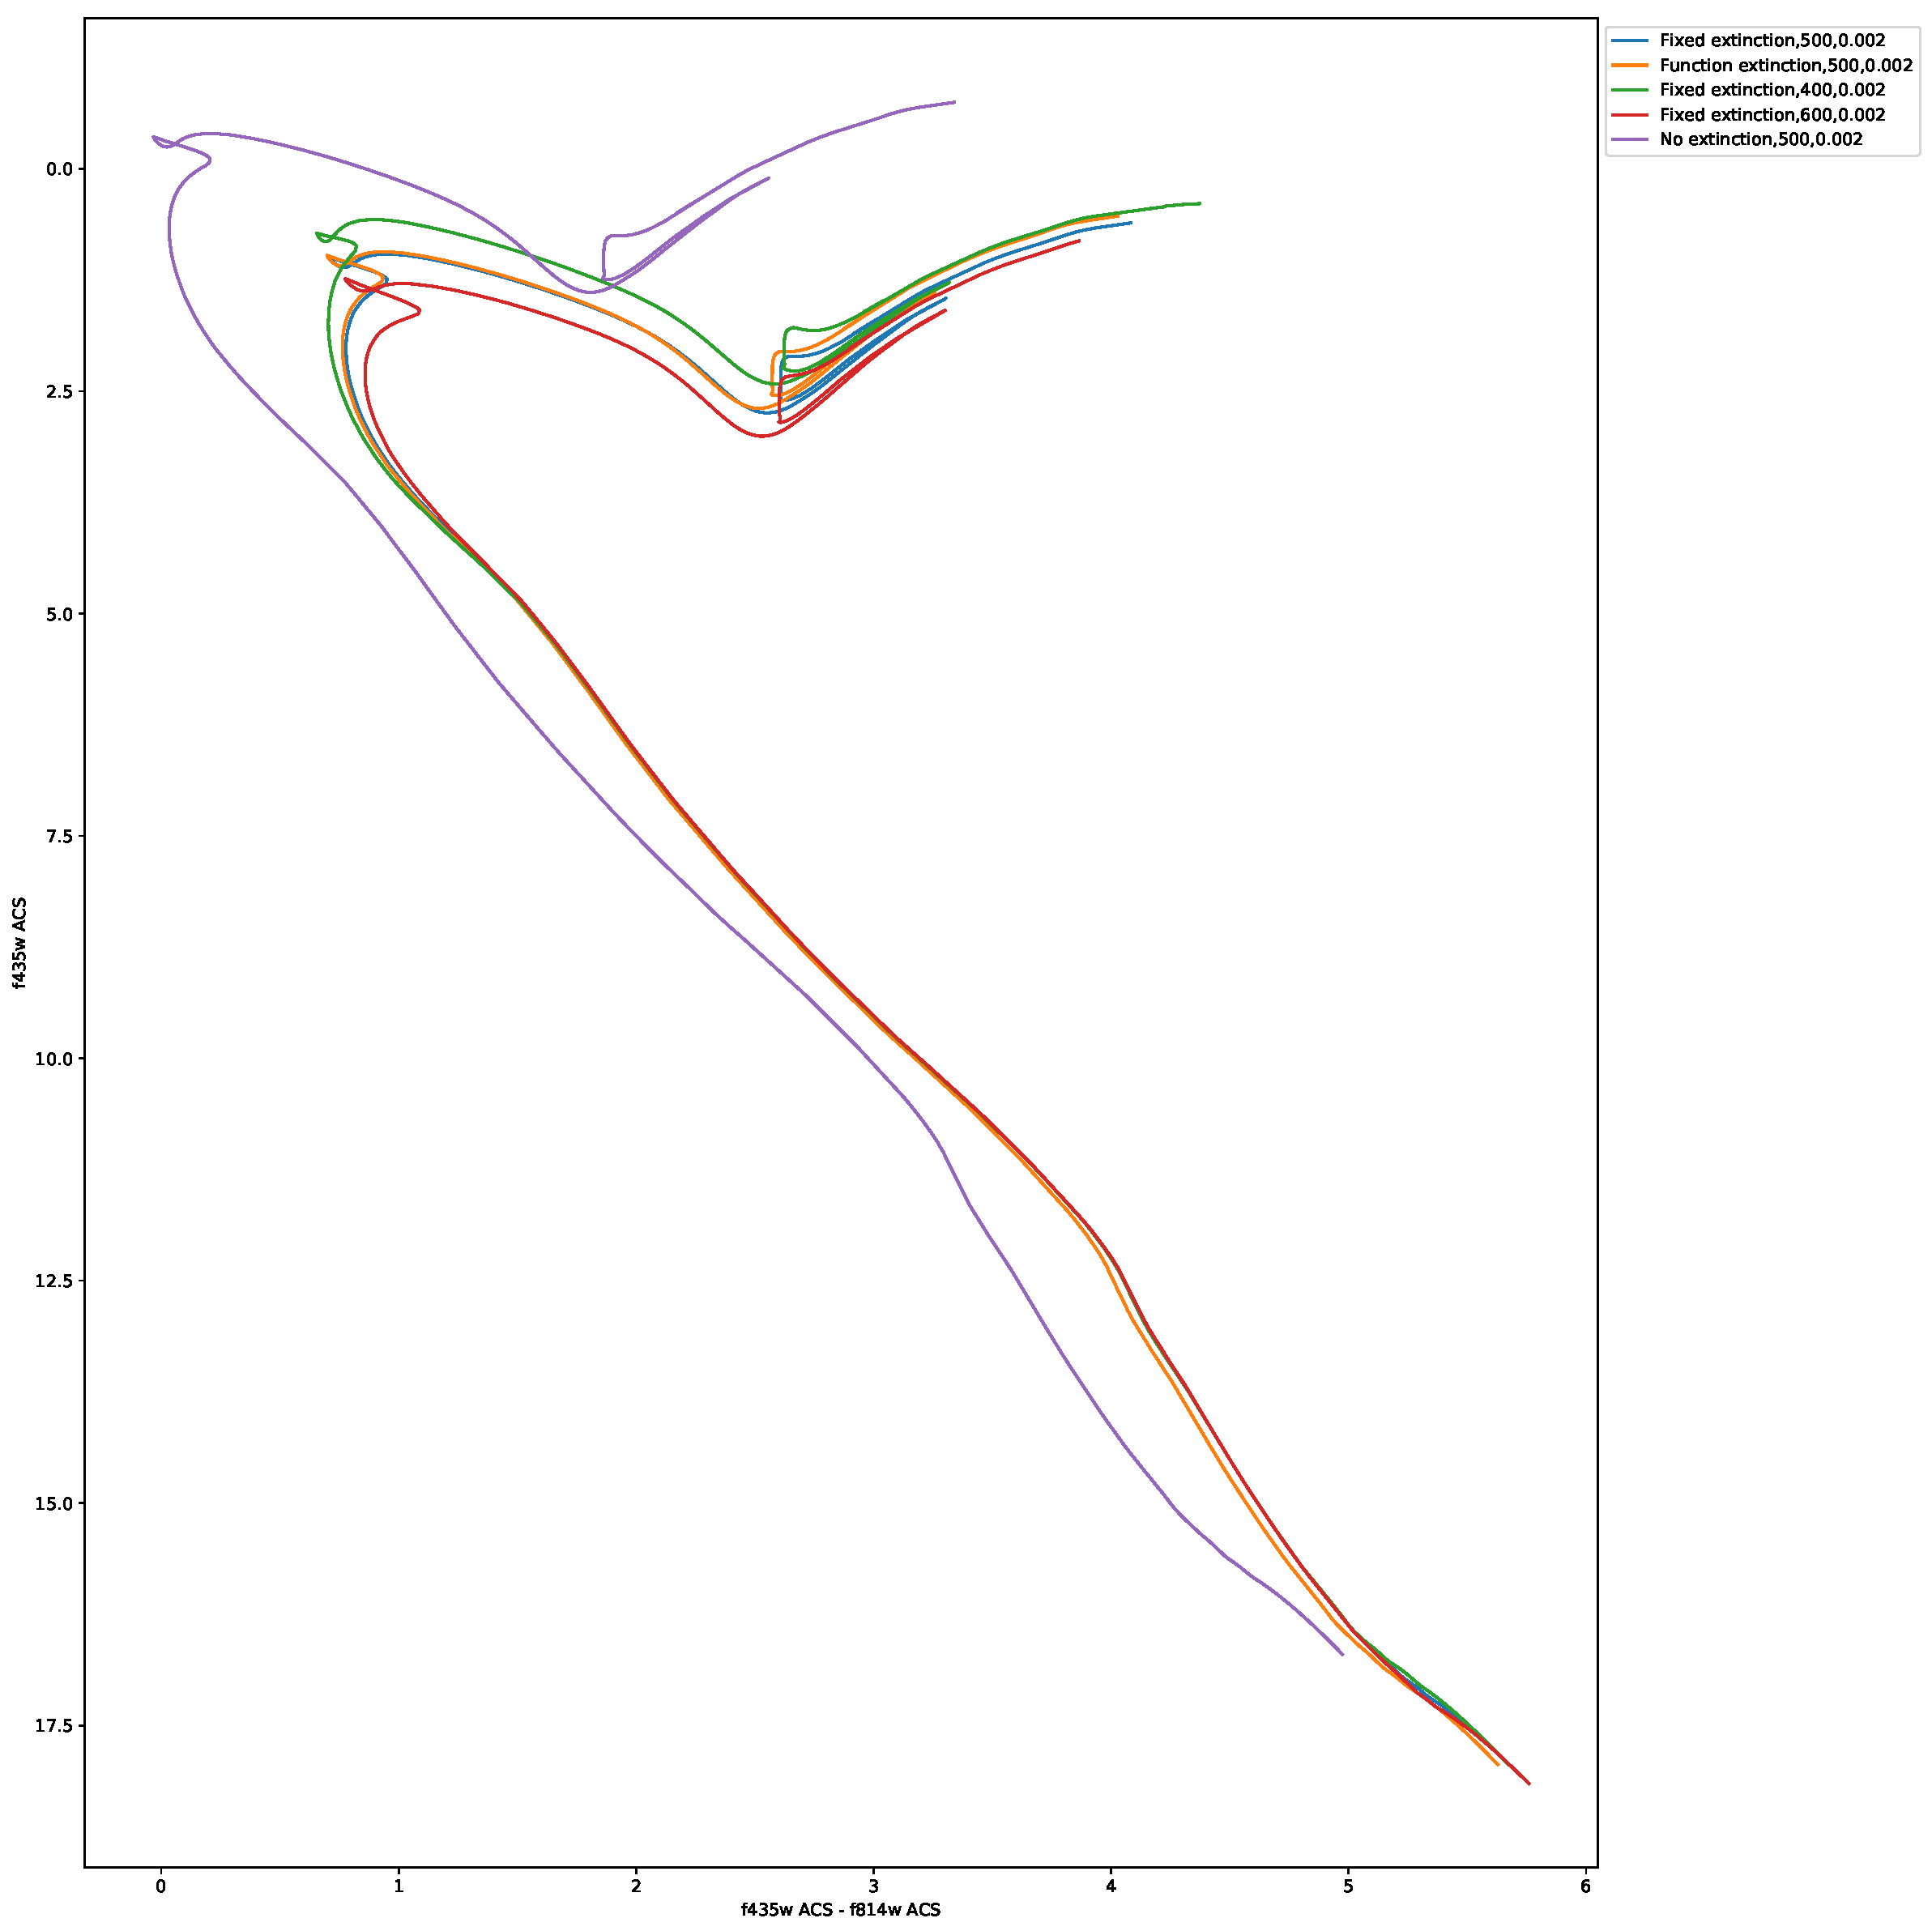
\includegraphics[scale=0.3]{../basti_isochrones_10_13Gyr/Extinction_T50k_FeH0fix_func_f435wACS_f435wACSmf814wACS_500_400_600_Myr_FeH_0p002_ref_noext_Av_1p0.pdf}
\caption{ACS F435W-(F435W-F814W) CMD with a fixed extinction coefficient equal to $(A_{X}/A_{V})_{plat}$ for each filter}
\label{acs_isoc_T50k}
\end{center}
\end{figure}

\subsection{WFC3} \label{WFC3_isoc}

The CMD chosen for the ACS was the F435W-(F435W-F814W) axis combination. This CMD is useful as it pairs the bluest and reddest wide-field filters for the ACS, which produces larger spectral colours.****

\begin{figure}[h]
\begin{center}
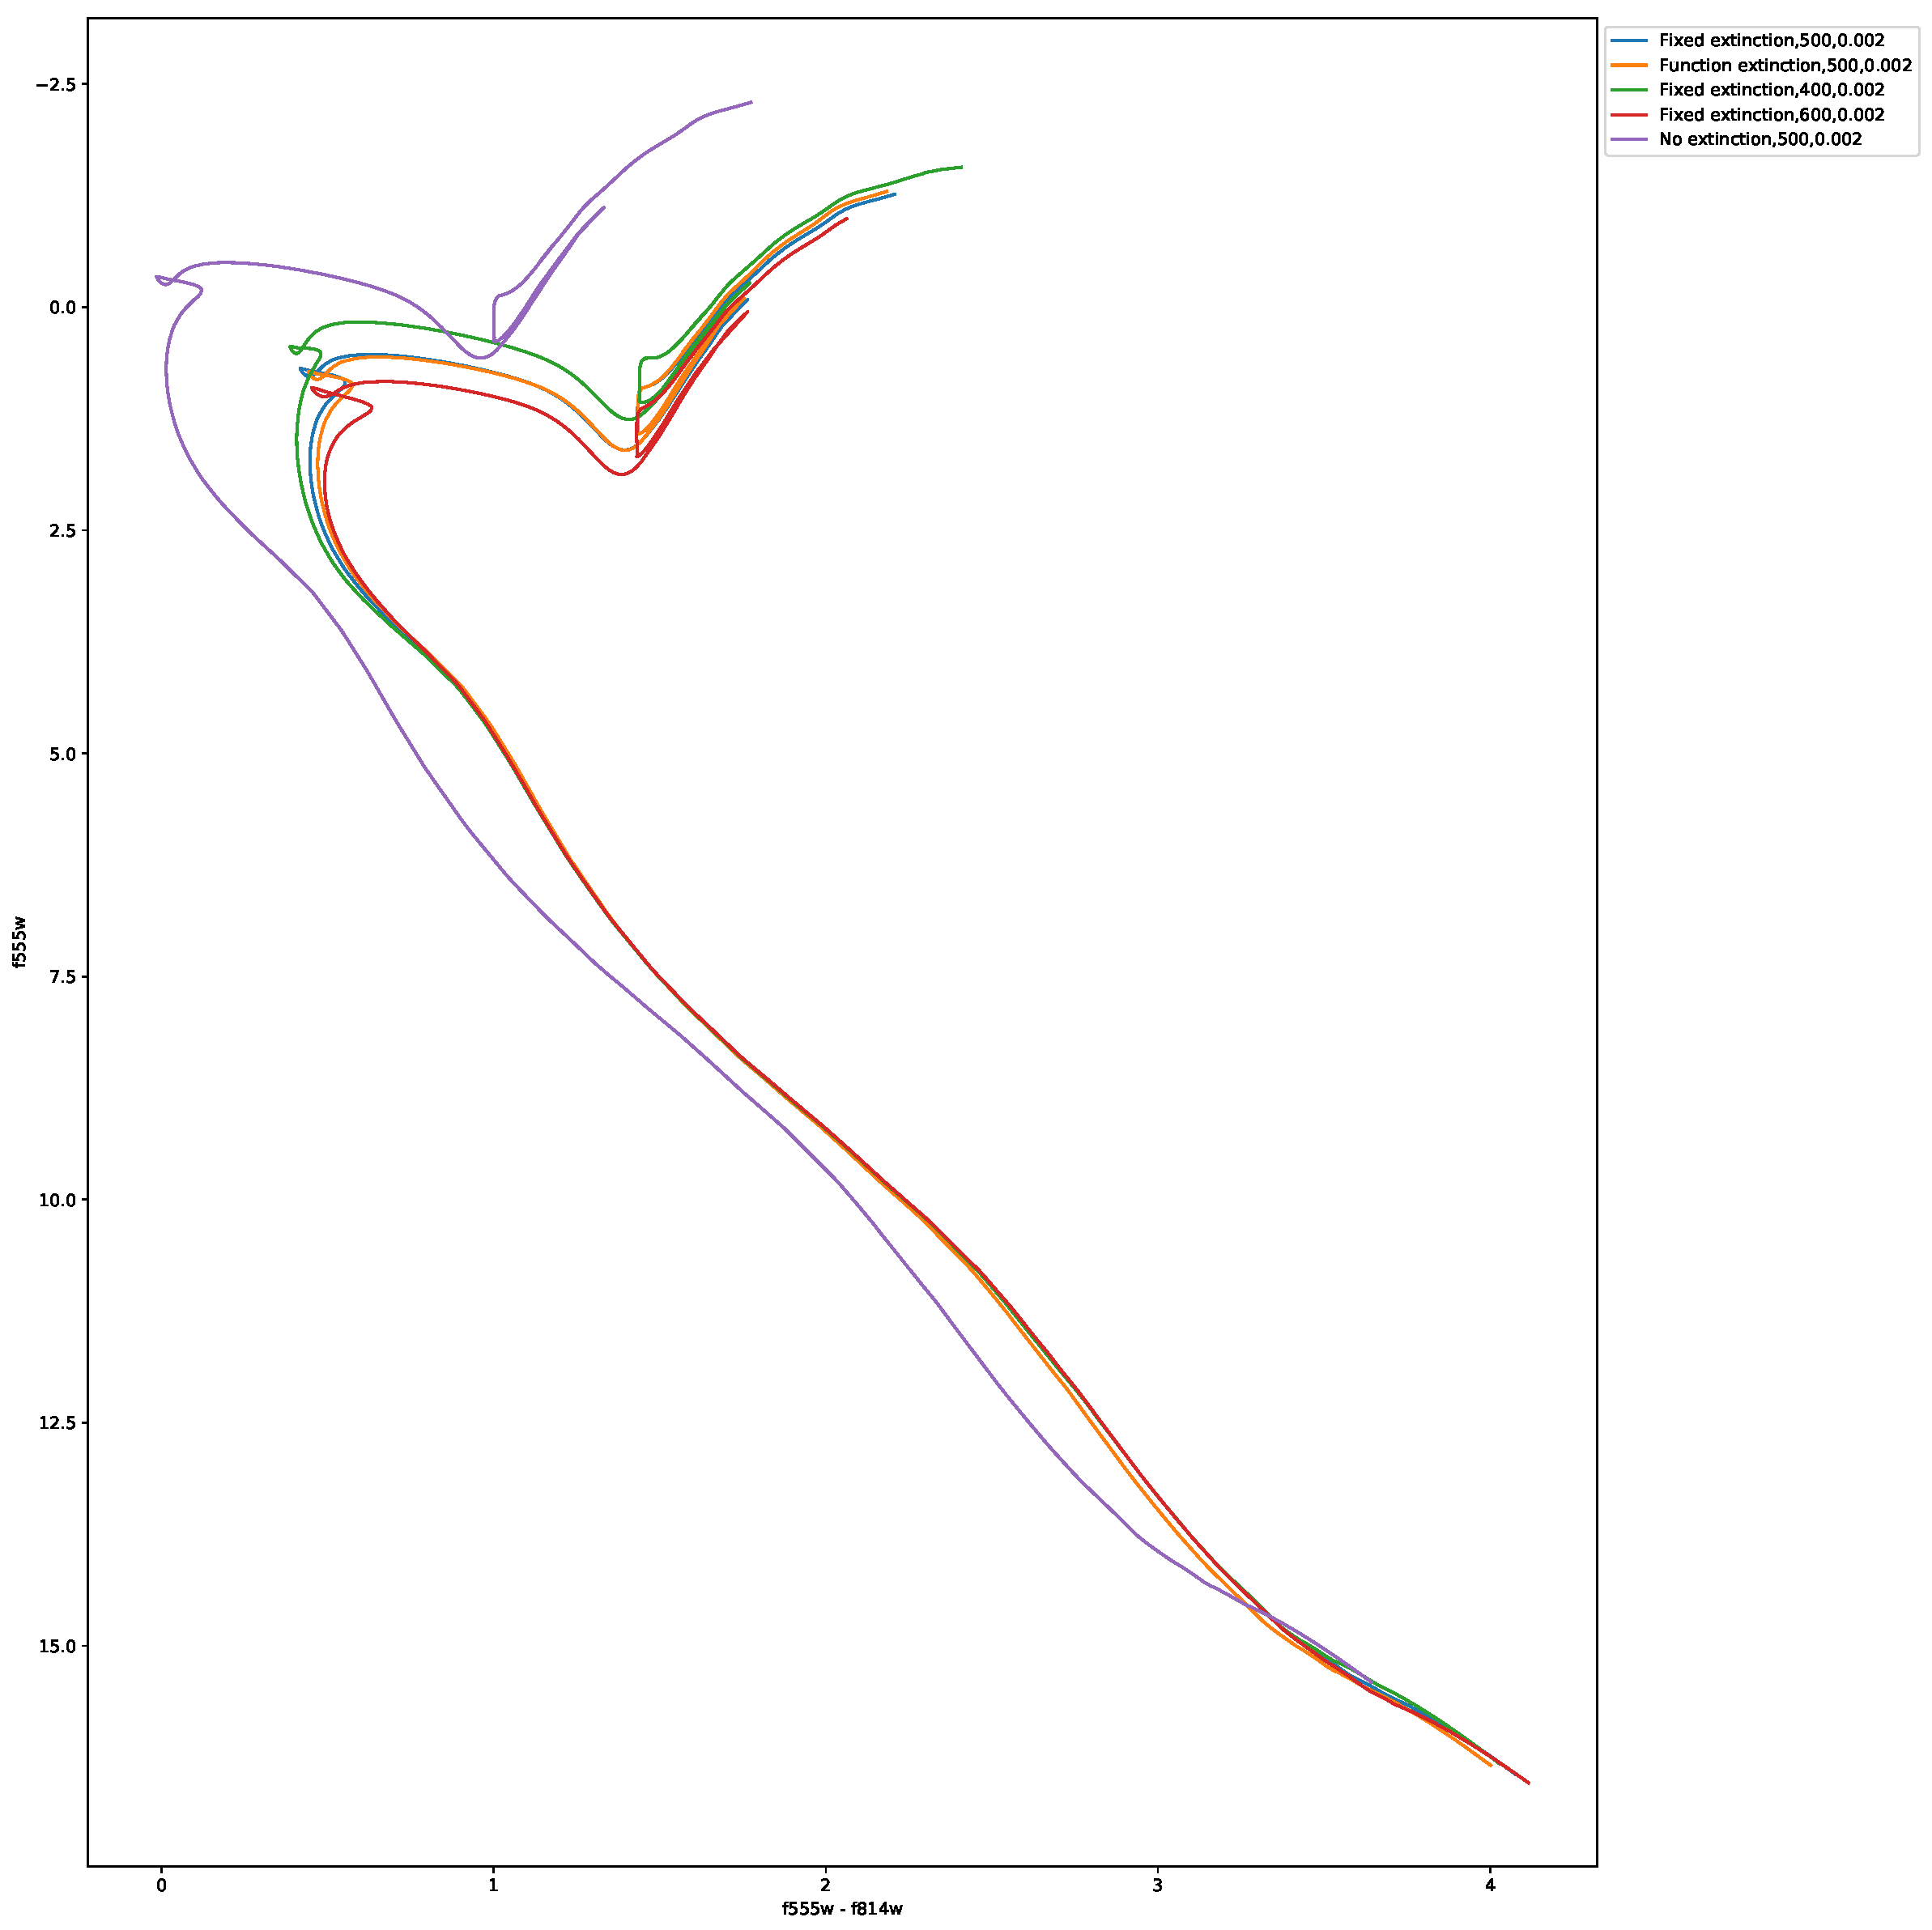
\includegraphics[scale=0.3]{../basti_isochrones_10_13Gyr/Extinction_T5k_FeH0fix_func_f555w_f555wmf814w_500_400_600_Myr_FeH_0p002_ref_noext_Av_1p0.pdf}
\caption{WFC3 F555W-(F555W-F814W) CMD with a fixed extinction coefficient equal to $(A_{X}/A_{V})_{MS}$ for each filter}
\label{wfc3_isoc1_T5k}
\end{center}
\end{figure}

\begin{figure}[h]
\begin{center}
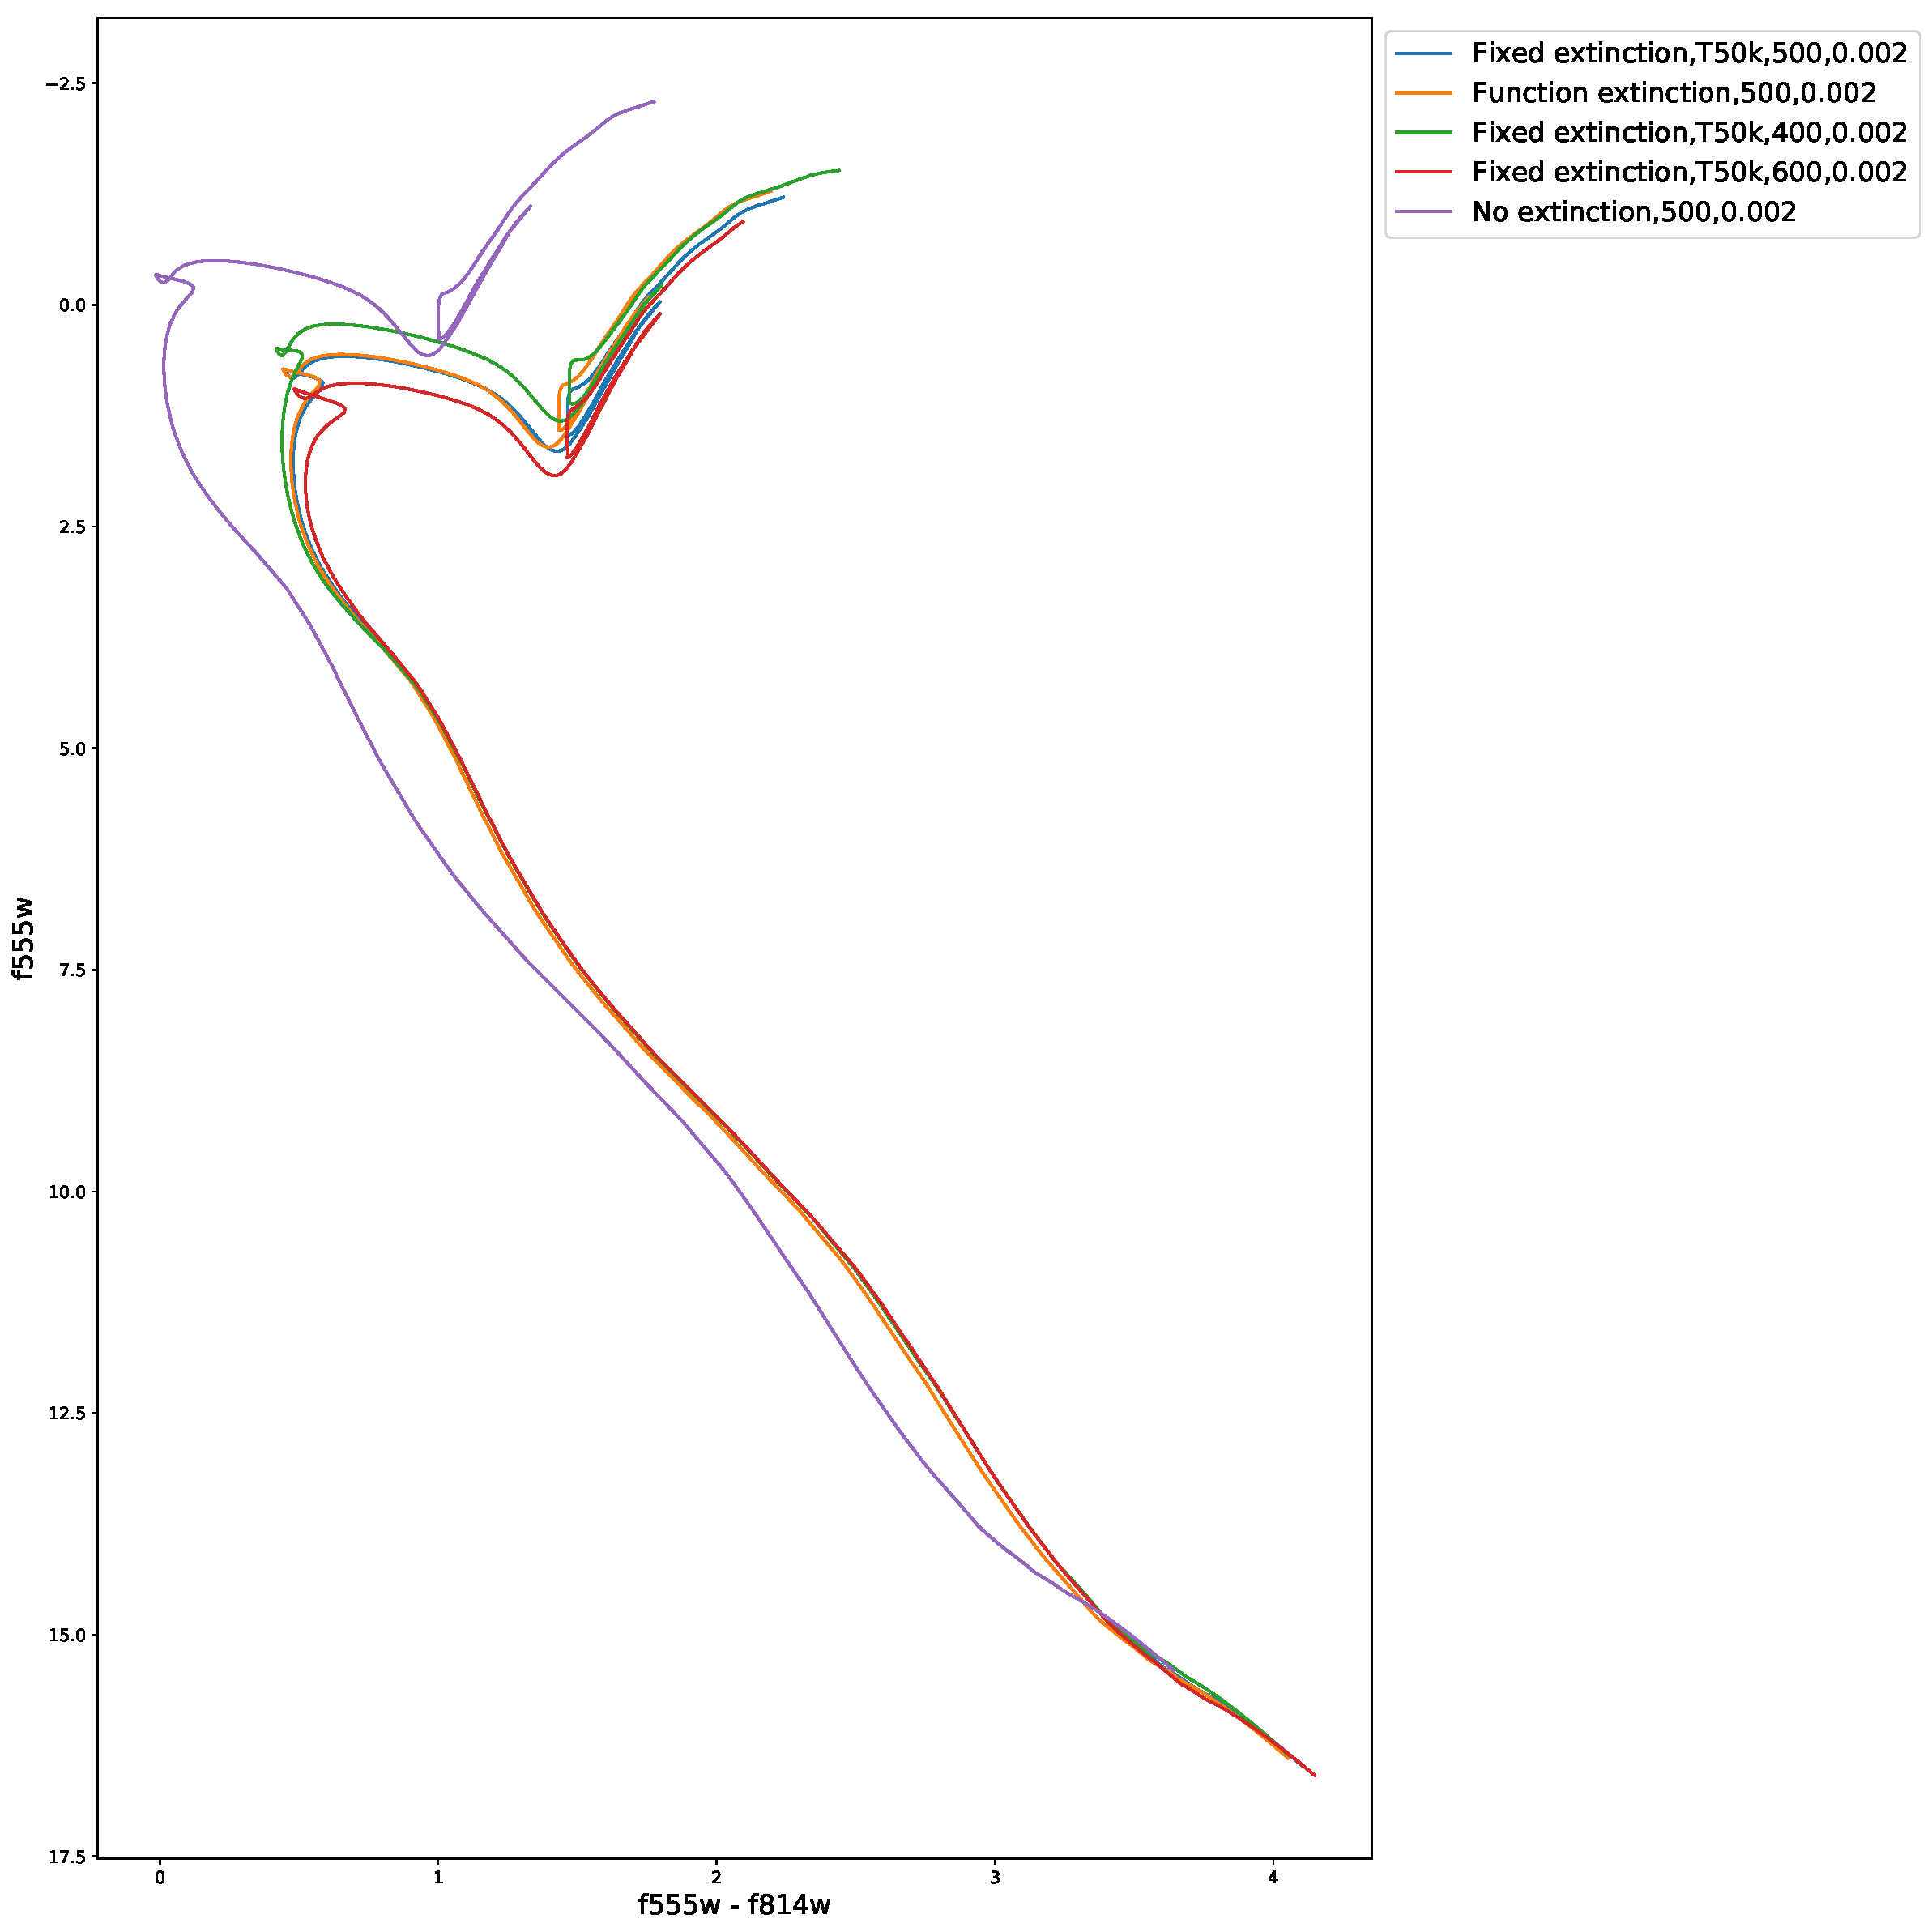
\includegraphics[scale=0.3]{../basti_isochrones_10_13Gyr/Extinction_T50k_FeH0fix_func_f555w_f555wmf814w_500_400_600_Myr_FeH_0p002_ref_noext_Av_1p0.pdf}
\caption{WFC3 F555W-(F555W-F814W) CMD with a fixed extinction coefficient equal to $(A_{X}/A_{V})_{plat}$ for each filter}
\label{wfc3_isoc1_T50k}
\end{center}
\end{figure}

\begin{figure}[h]
\begin{center}
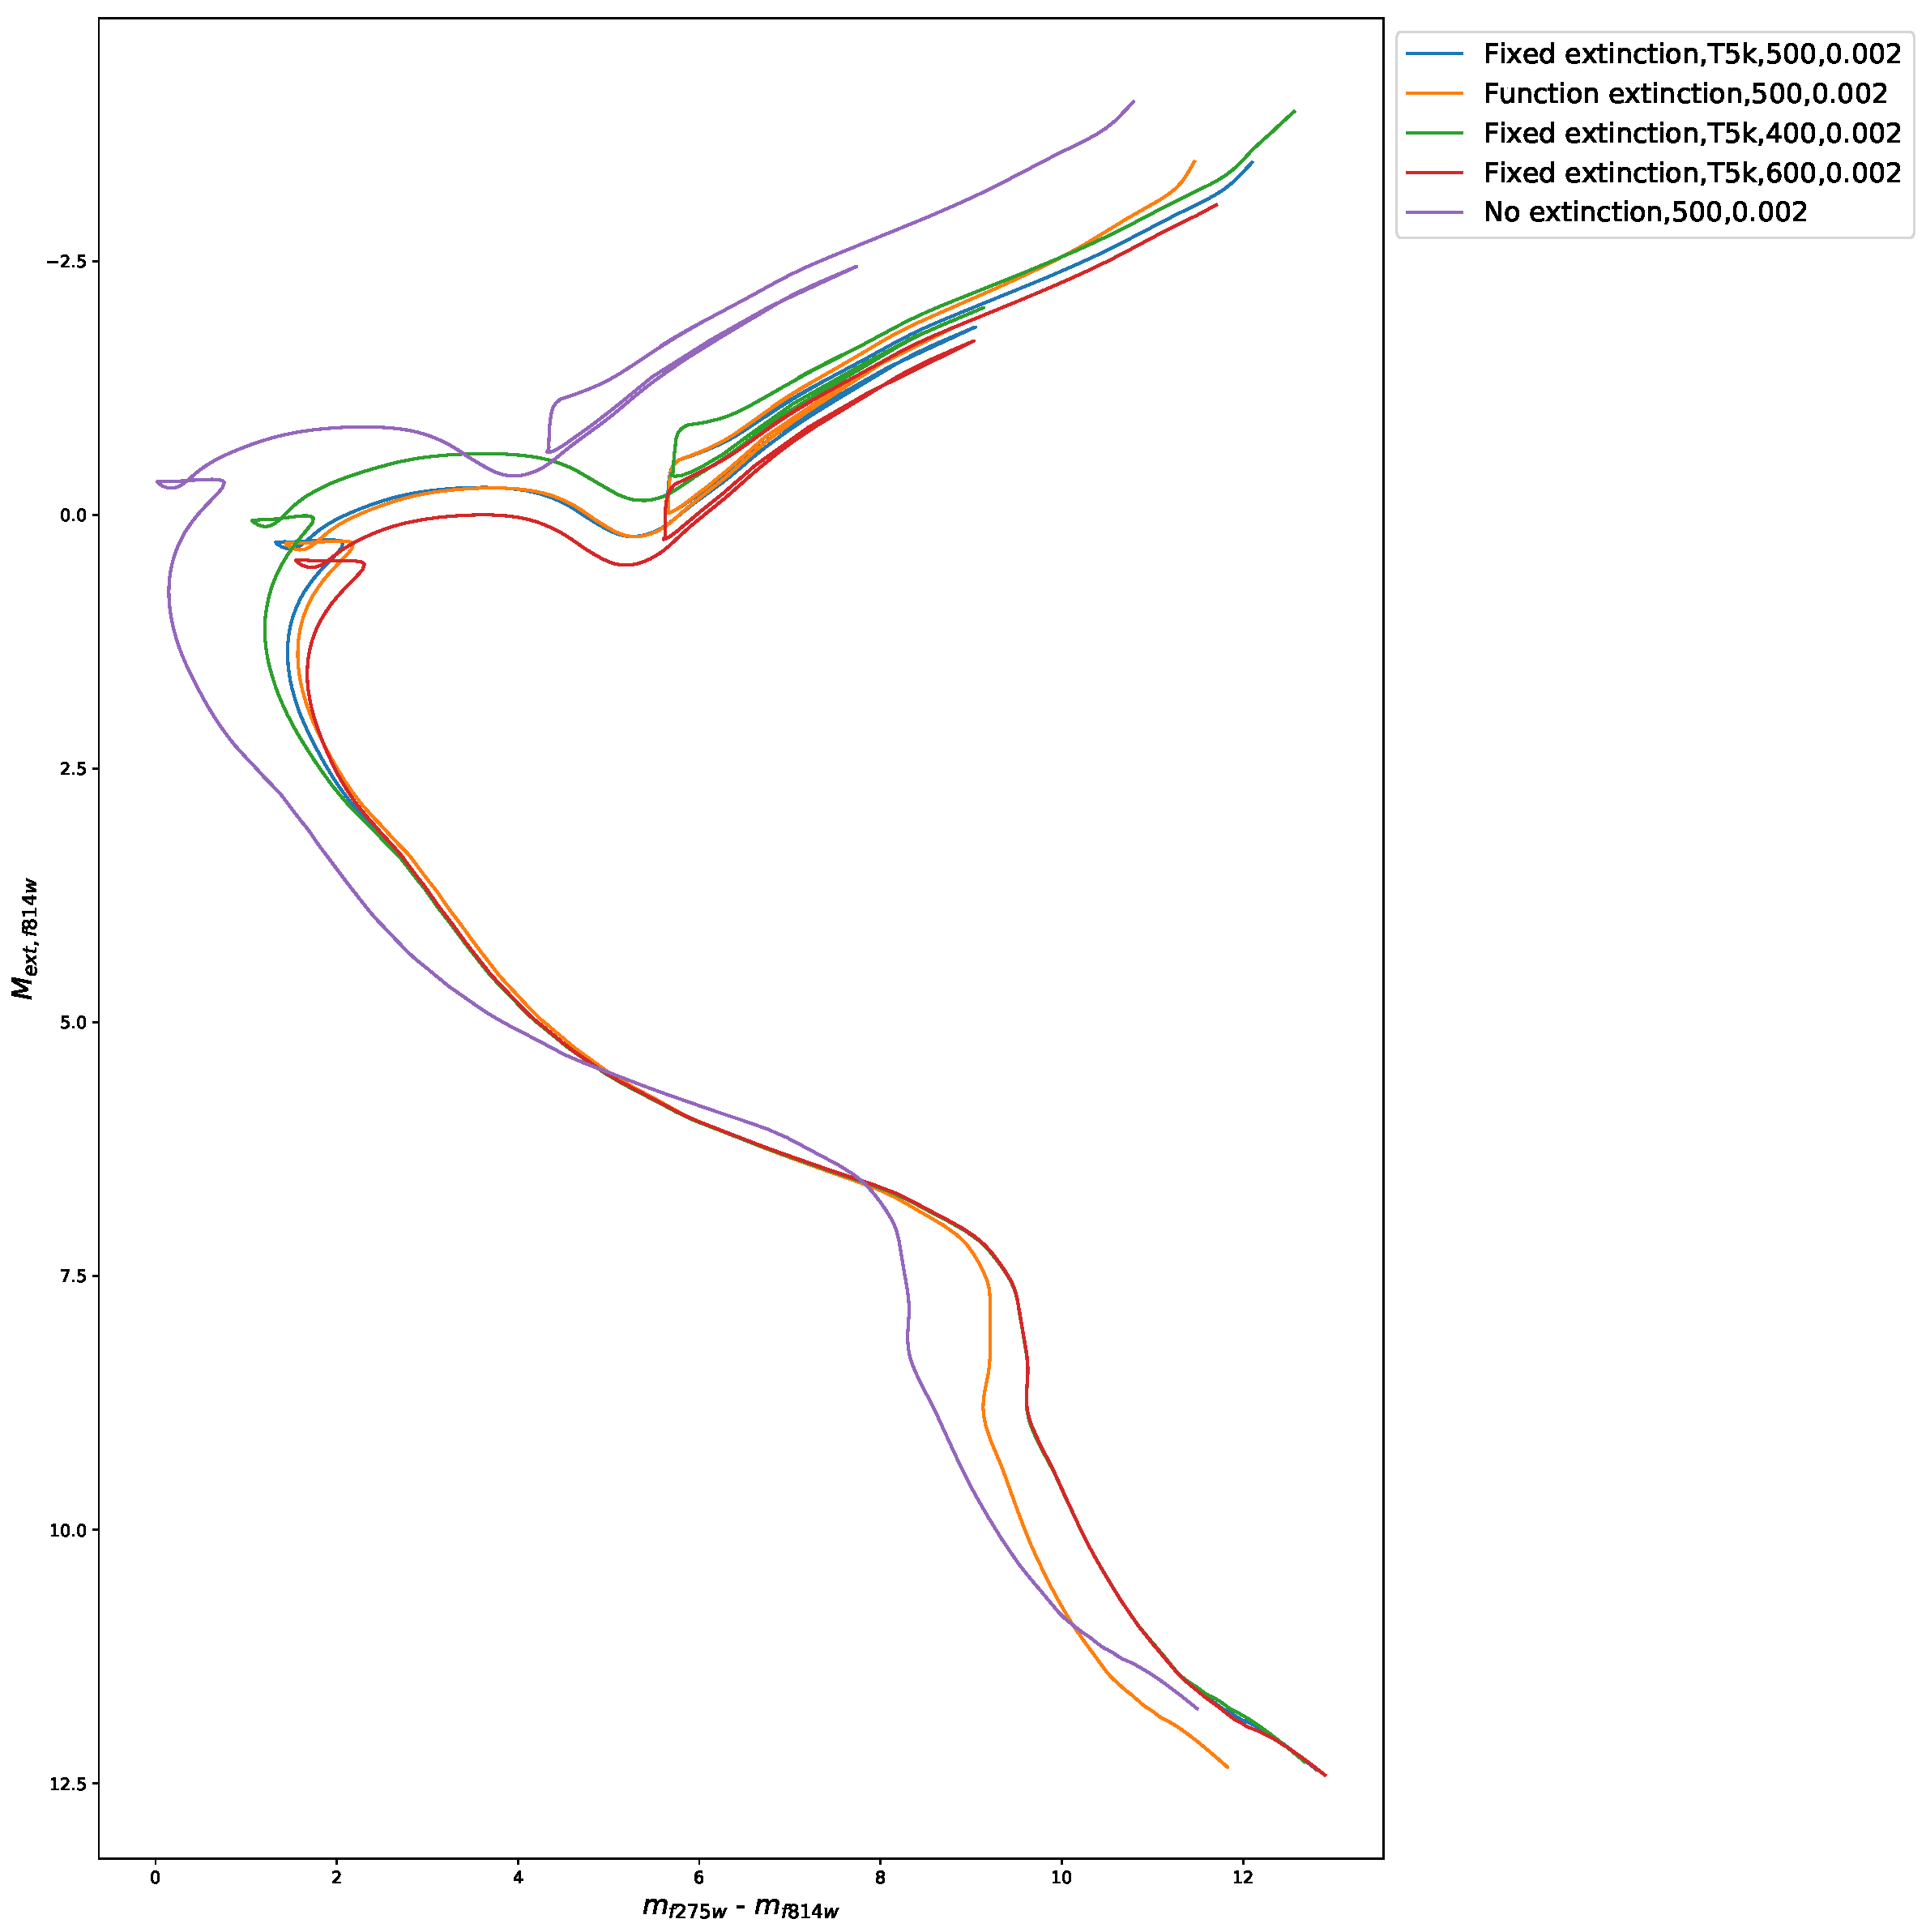
\includegraphics[scale=0.3]{../basti_isochrones_10_13Gyr/Extinction_T5k_FeH0fix_func_f814w_f275wmf814w_500_400_600_Myr_FeH_0p002_ref_noext_Av_1p0.pdf}
\caption{WFC3 F814W-(F275W-F814W) CMD with a fixed extinction coefficient equal to $(A_{X}/A_{V})_{MS}$ for each filter}
\label{wfc3_isoc2_T5k}
\end{center}
\end{figure}

\begin{figure}[h]
\begin{center}
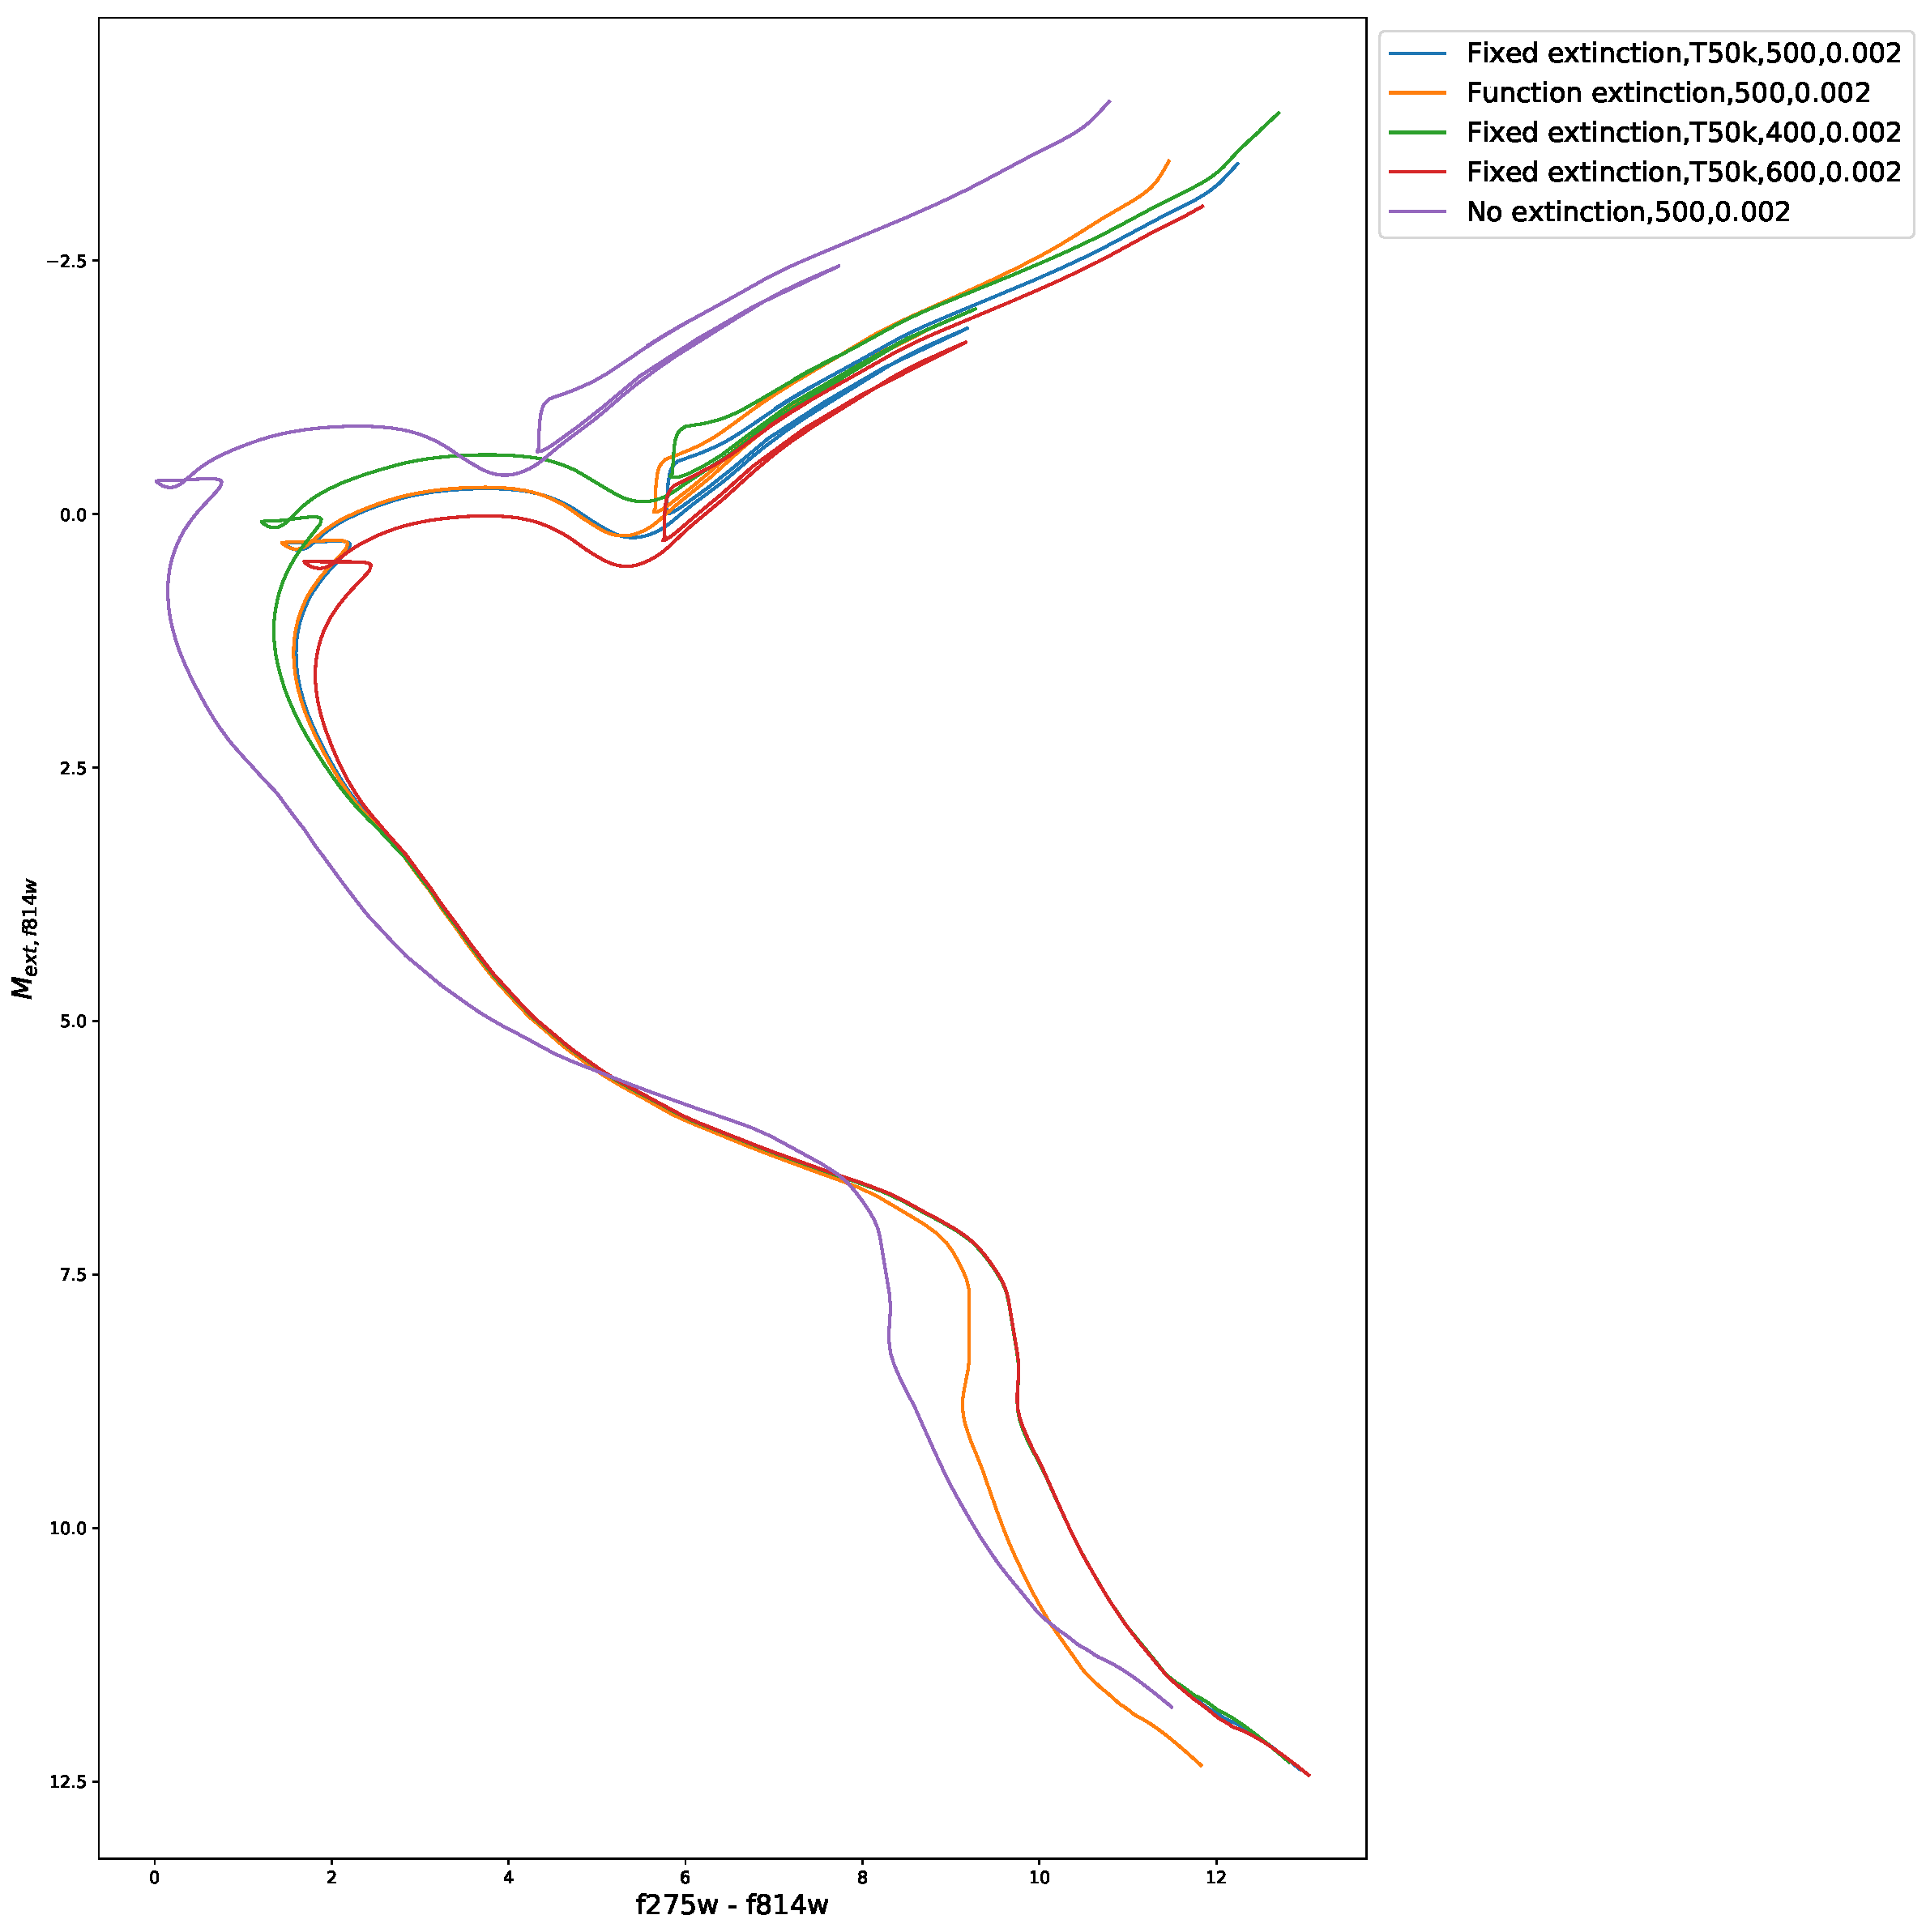
\includegraphics[scale=0.3]{../basti_isochrones_10_13Gyr/Extinction_T50k_FeH0fix_func_f814w_f275wmf814w_500_400_600_Myr_FeH_0p002_ref_noext_Av_1p0.pdf}
\caption{WFC3 F814W-(F275W-F814W) CMD with a fixed extinction coefficient equal to $(A_{X}/A_{V})_{plat}$ for each filter}
\label{wfc3_isoc2_T50k}
\end{center}
\end{figure}

\subsection{Gaia} \label{Gaia_isoc}

The photometric filters in Gaia, as shown by their respective response functions in Figure \ref{Gaia_response_funcs}, are designed such that the only reasonable colour index is the ($G_{\textnormal{bp}}-G_{\textnormal{rp}}$) index. The $G$ filter, being the widest filter of the three available wide-field filters. This CMD is useful as it pairs the bluest and reddest wide-field filters for the ACS, which produces larger spectral colours.****

\begin{figure}[h]
\begin{center}
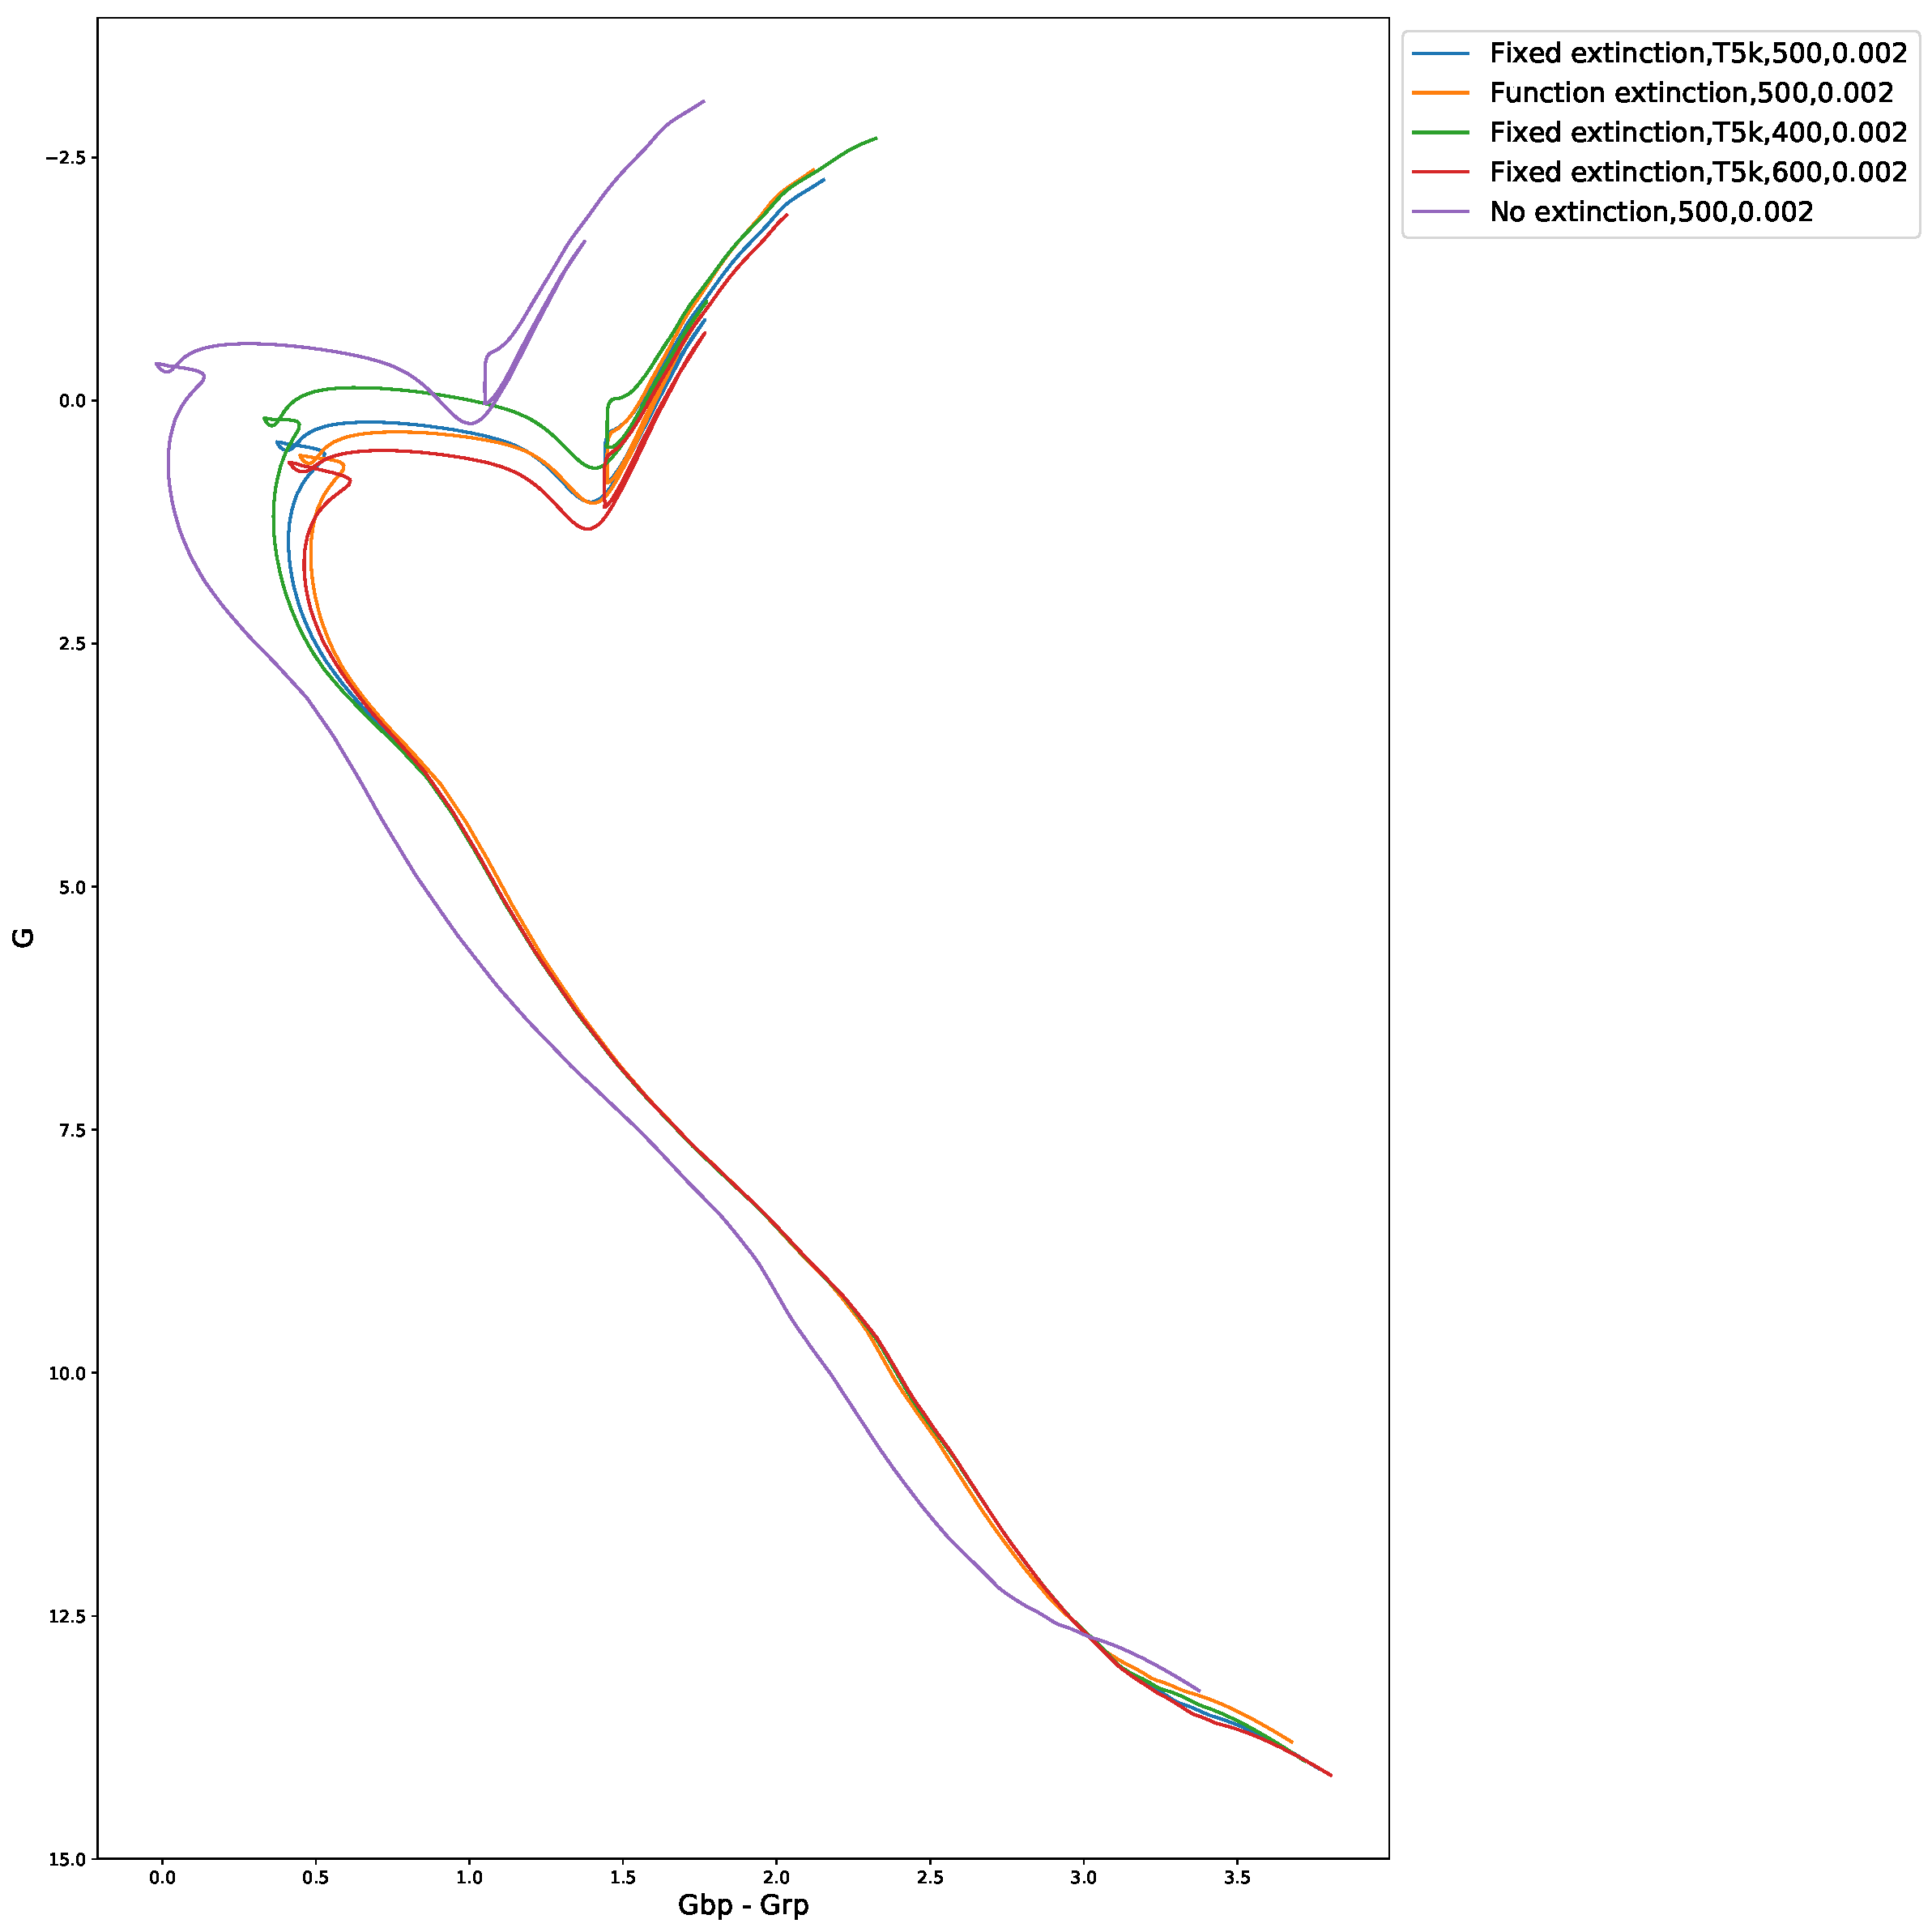
\includegraphics[scale=0.3]{../basti_isochrones_10_13Gyr/Extinction_T5k_FeH0fix_func_G_GbpmGrp_500_400_600_Myr_FeH_0p002_ref_noext_Av_1p0.pdf}
\caption{Gaia $G$-($G_{\textnormal{bp}}$-$G_{\textnormal{rp}}$) CMD with a fixed extinction coefficient equal to $(A_{X}/A_{V})_{MS}$ for each filter}
\label{gaia_isoc_T5k}
\end{center}
\end{figure}

\begin{figure}[h]
\begin{center}
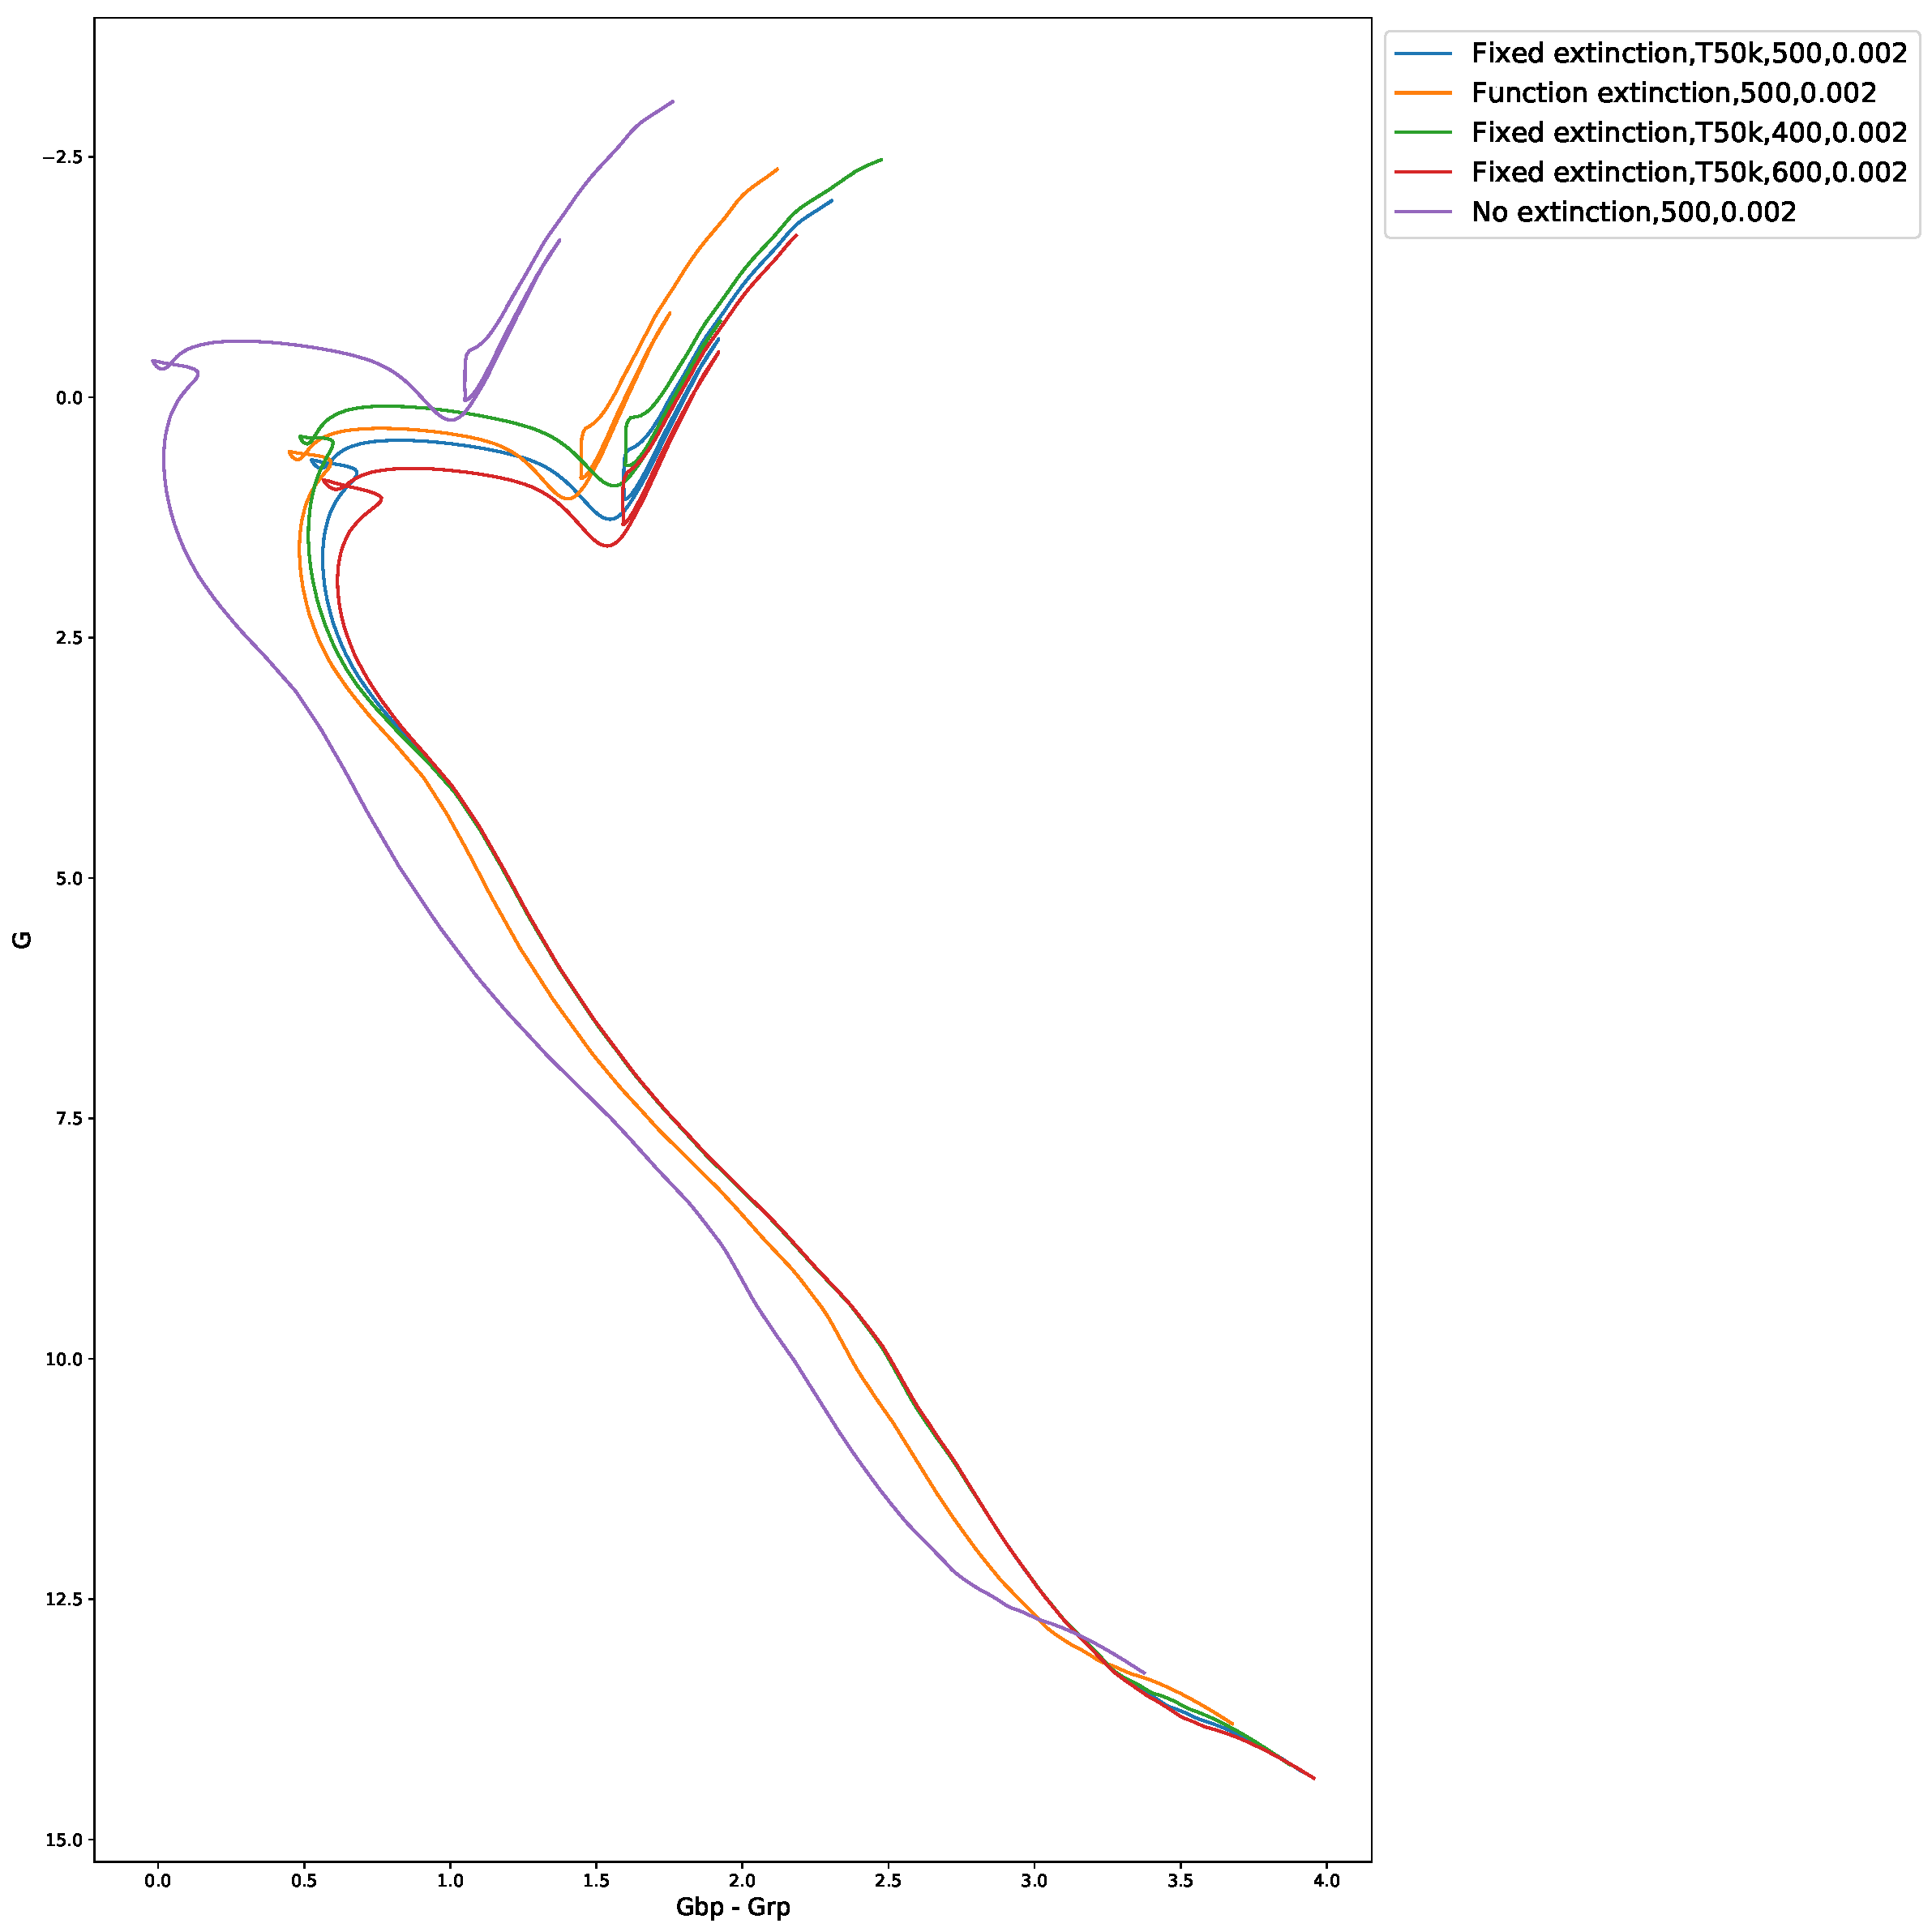
\includegraphics[scale=0.3]{../basti_isochrones_10_13Gyr/Extinction_T50k_FeH0fix_func_G_GbpmGrp_500_400_600_Myr_FeH_0p002_ref_noext_Av_1p0.pdf}
\caption{Gaia $G$-($G_{\textnormal{bp}}$-$G_{\textnormal{rp}}$) CMD with a fixed extinction coefficient equal to $(A_{X}/A_{V})_{plat}$ for each filter}
\label{gaia_isoc_T50k}
\end{center}
\end{figure}

\section{NGC 6793}

\begin{figure}[h]
\begin{center}
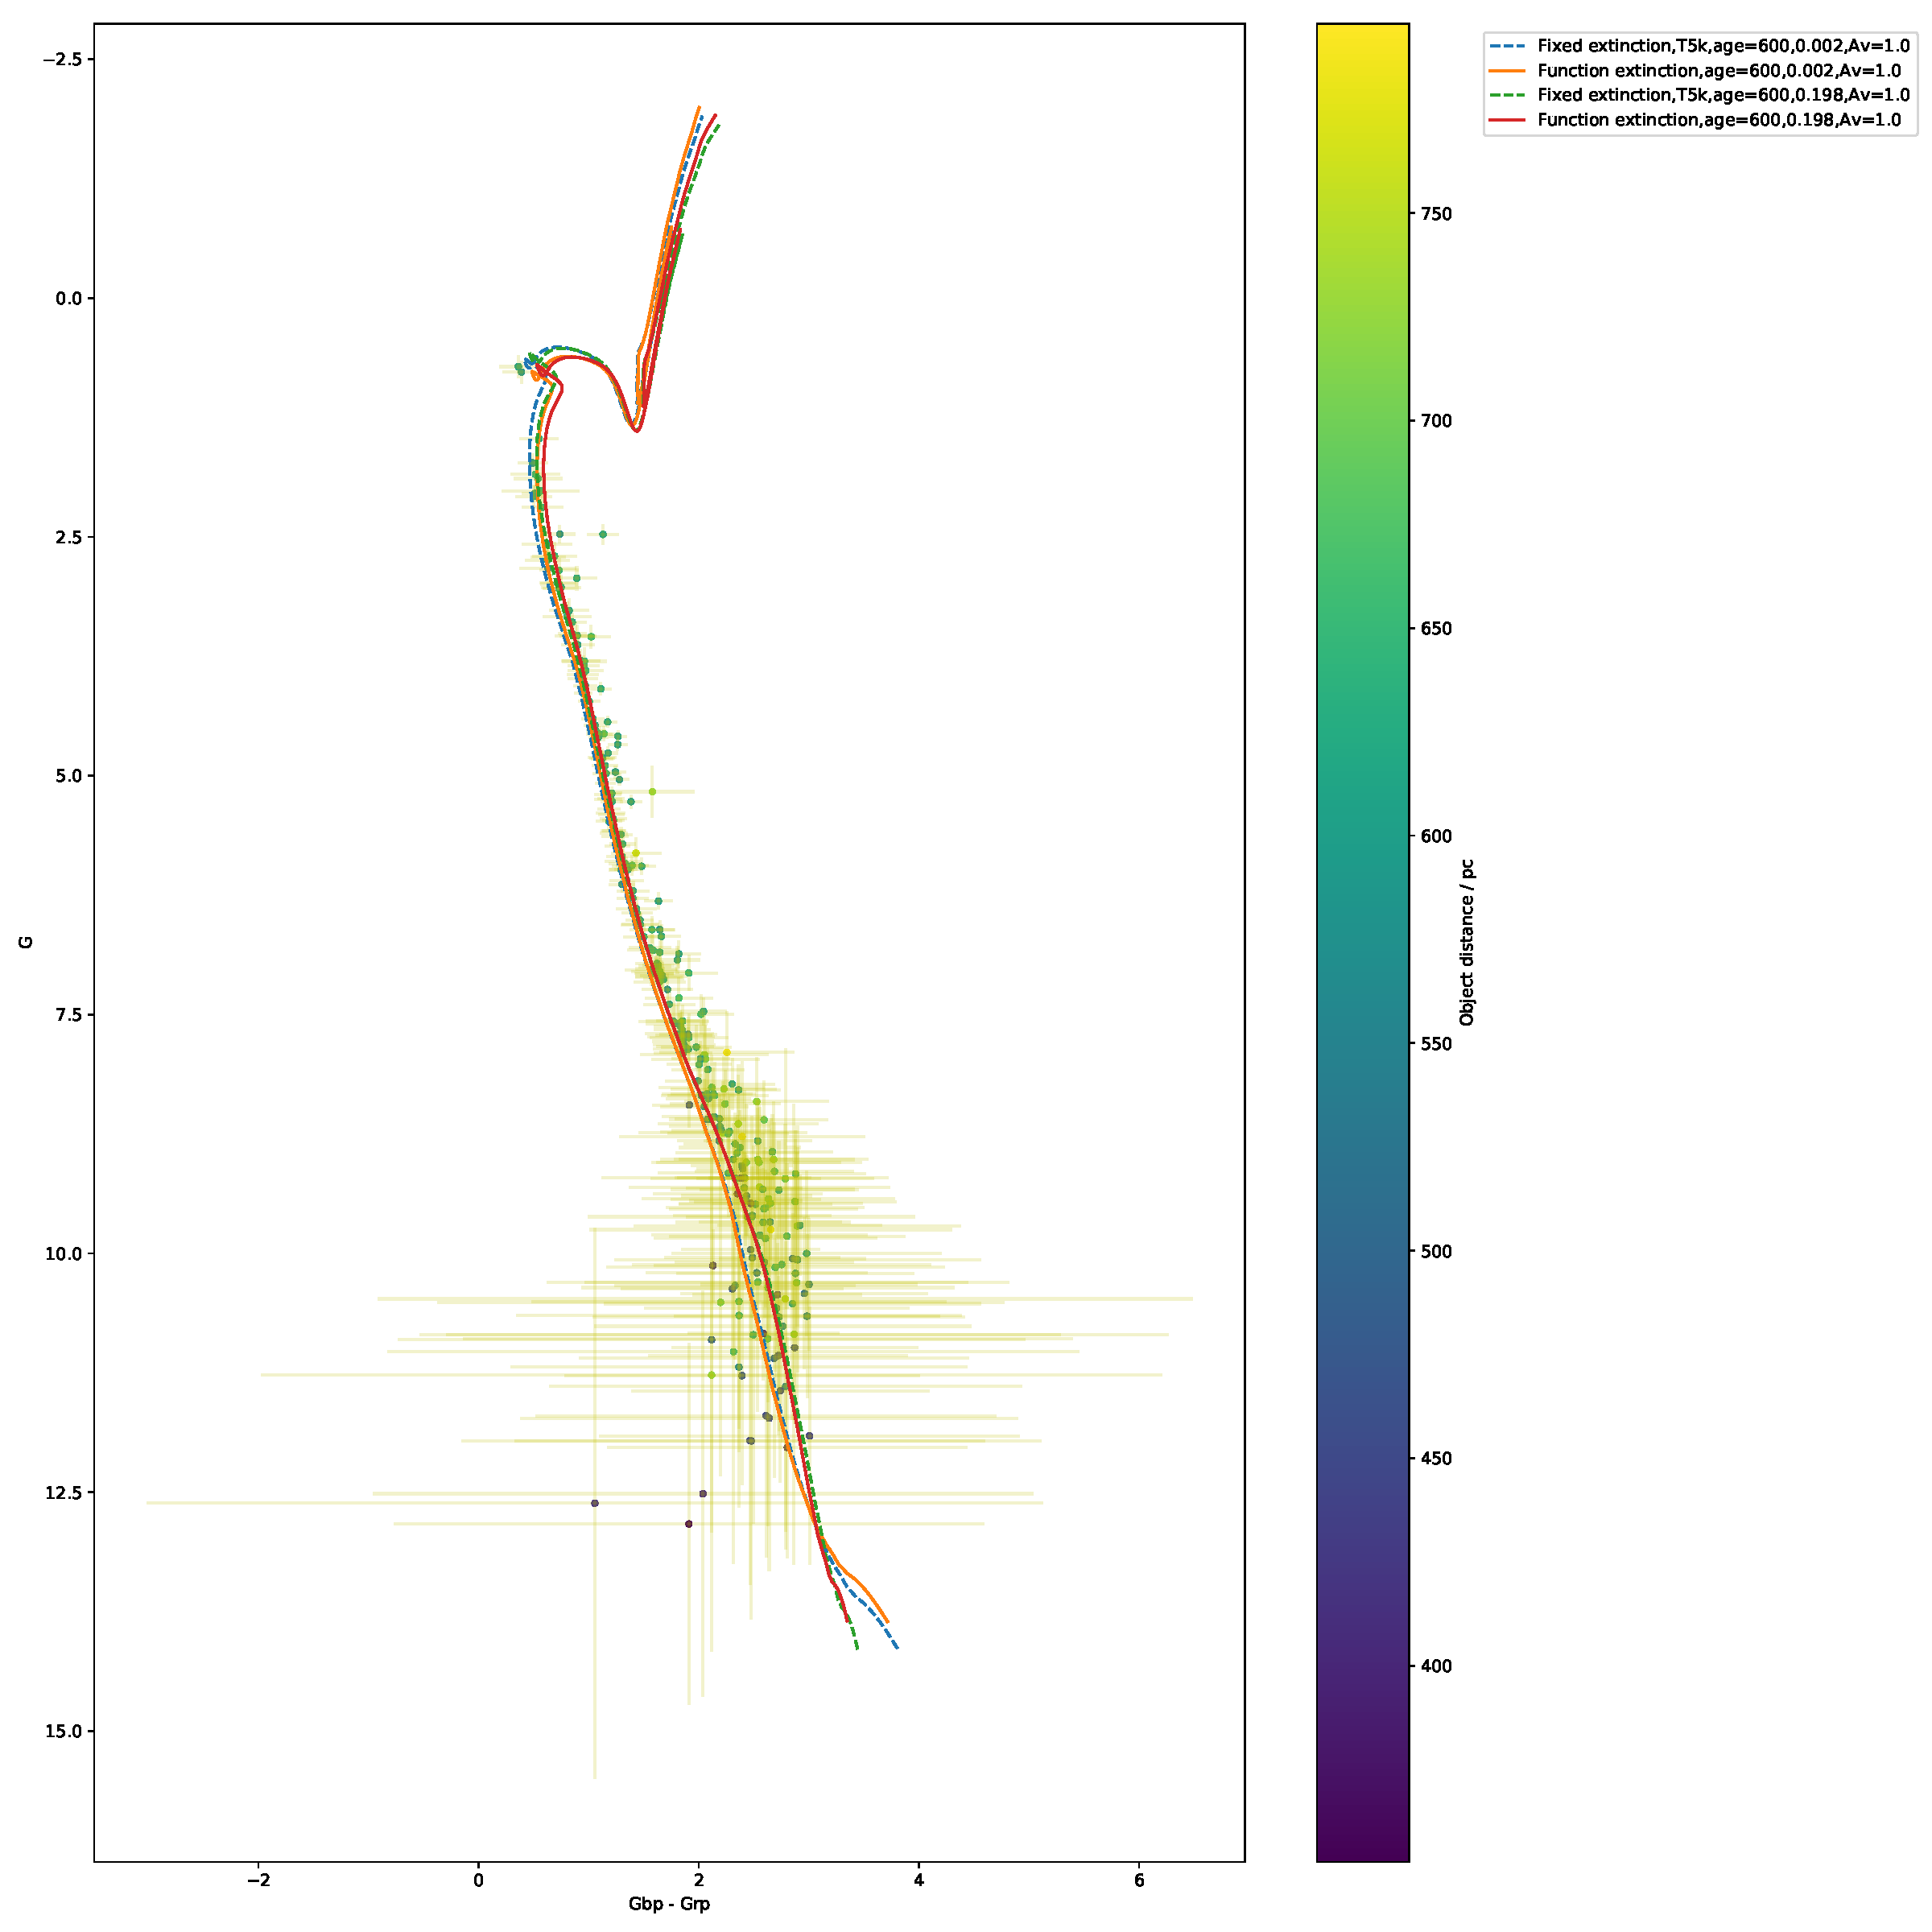
\includegraphics[scale=0.3]{../NGC_6793_CMD_FeH_0p002_0p198_Av_1p0_600Myr_isochrones_both_errorbars_T5k.pdf}
\caption{Gaia CMD of NGC 6793 with errorbars included.}
\label{ngc_errorbars}
\end{center}
\end{figure}

There are highly significant errors for the individual objects in the Gaia data propagation, even when assuming the only source of error is from  parallax measurements, as shown in Figure \ref{ngc_errorbars}. The magnitude of the errorbars dwarf any changes in isochrones due to extinction coefficient treatments in the main sequence. For the few objects in the data with 

****Get zoom in on turn-off region

All the isochrones, as shown in Section****, are sensitive both to the reference extinction coefficient value $A_{V}$ and to the value of $A_{X}/A_{V}$ for the fixed-coefficient case, which is to be expected. Some individual parts of the isochrones relevant to this study are additionally sensitive to other isochrone parameters:

\begin{enumerate}
%, but metallicity has a smaller effect
\item The position of the MSTO is sensitive to the treatment of $A_{X}/A_{V}$, as shown in Section****, and the isochrone age.
\item The position of the lower main sequence is significantly more sensitive to metallicity than other parts of the isochrone.
\end{enumerate}



\chapter{Conclusion}
In all cases, applying a fixed extinction to all points in an isochrone causes the main-sequence turn-off to occur at a more luminous, bluer point in a given CMD than the MSTO point for an extinction coefficient described using a function fitted to empirically derived data.

\section{Future work}

%\bibliographystyle{ieeetr}
\bibliographystyle{mnras} % unsrtnat
\bibliography{mphil_thesis}

\end{document}